%%%%%%%%%%%%%%%%%%%%%   TABLES     %%%%%%%%%%%%%%%%%%%%%%%%%%%%%%%%%%%%%%%%%%%%%

\section{Tables}

% latex table generated in R 3.1.1 by xtable 1.7-4 package
% Fri Dec 19 13:50:59 2014
\begin{landscape}
\begin{longtable}{lll}
\caption{The agricultural land cover classes represented within SWAT are shown here with the class of land use and land management. The rotation codes are Cg=corn grain, Cs=corn silage, So=soybean, Po=potato, Vg=vegetable, A=Alfalfa, O/A=oats/alfalfa. Tons are English tons.} 
 %%%%%%%%%%%%%%%%%%%%%%%%%%%%%%%%%%%%%%
\hline 
%%%First and actual col titles
	SWAT Landuse & Type & Definition  \\ 
 \hline 
 \hline
\endfirsthead
%%%%% repeating head
	\multicolumn{3}{c}%
		{\tablename\ \thetable\ -- \textit{Continued from previous page}} \hline \\
SWAT Landuse & Type & Definition  \\ 
	\hline 
	\hline 
\endhead

		\hline \multicolumn{3}{r}{\textit{Continued on next page}} \\
	\endfoot

	\hline
	\endlastfoot
%%%%%%%%%%%%%%%%%%%%%%%%%%%%%%%%%%%%%%%%%%%%% 
  SWHT & Dairy & Cg-Cs-O/A-A-A-A - Spring Chisel - 10,000 ga/acre/year Liquid Manure  \\ 
  WWHT & Dairy & O/A-A-A-A-Cg-Cs - Spring Chisel - 10,000 ga/acre/year Liquid Manure  \\ 
  DWHT & Dairy & A-A-Cg-Cs-O/A-A - Spring Chisel - 10,000 ga/acre/year Liquid Manure  \\ 
  RYE & Dairy & Cg-Cs-O/A-A-A-A - Spring Chisel - 25 tons/acre/year Solid Manure  \\ 
  BARL & Dairy & O/A-A-A-A-Cg-Cs - Spring Chisel - 25 tons/acre/year Solid Manure  \\ 
  OATS & Dairy & A-A-Cg-Cs-O/A-A - Spring Chisel - 25 tons/acre/year Solid Manure  \\ 
  RICE & Dairy & Cg-O/A-A-A-A-A - Spring Chisel - 25 tons/acre/year Solid Manure  \\ 
  PMIL & Dairy & A-A-A-A-Cg-O/A - Spring Chisel - 25 tons/acre/year Solid Manure  \\ 
  TIMO & Dairy & A-A-Cg-O/A-A-A - Spring Chisel - 25 tons/acre/year Solid Manure  \\ 
  BROS & Dairy & Cg-Cs-O/A-A-A-A - Fall Chisel - 10,000 ga/acre/year Liquid Manure  \\ 
  BROM & Dairy & O/A-A-A-A-Cg-Cs - Fall Chisel - 10,000 ga/acre/year Liquid Manure  \\ 
  FESC & Dairy & A-A-Cg-Cs-O/A-A - Fall Chisel - 10,000 ga/acre/year Liquid Manure  \\ 
  BLUG & Dairy & Cg-Cs-O/A-A-A-A - Fall Chisel - 25 tons/acre/year Solid Manure  \\ 
  BERM & Dairy & O/A-A-A-A-Cg-Cs - Fall Chisel - 25 tons/acre/year Solid Manure  \\ 
  CWGR & Dairy & A-A-Cg-Cs-O/A-A - Fall Chisel - 25 tons/acre/year Solid Manure  \\ 
  WWGR & Dairy & Cs-Cs-O/A-A-A-A - Fall Chisel - 10,000 ga/acre/year Liquid Manure  \\ 
  SWGR & Dairy & O/A-A-A-A-Cs-Cs - Fall Chisel - 10,000 ga/acre/year Liquid Manure  \\ 
  RYEG & Dairy & A-A-Cs-Cs-O/A-A - Fall Chisel - 10,000 ga/acre/year Liquid Manure  \\ 
  RYER & Dairy & Cs-Cs-O/A-A-A-A - Fall Chisel - 25 tons/acre/year Solid Manure  \\ 
  RYEA & Dairy & O/A-A-A-A-Cs-Cs - Fall Chisel - 25 tons/acre/year Solid Manure  \\ 
  SIDE & Dairy & A-A-Cs-Cs-O/A-A - Fall Chisel - 25 tons/acre/year Solid Manure  \\ 
  BBLS & Dairy & Cs-Cs-O/A-A-A-A - Fall MB Plow - 10,000 ga/acre/year Liquid Manure  \\ 
  LBLS & Dairy & O/A-A-A-A-Cs-Cs - Fall MB Plow - 10,000 ga/acre/year Liquid Manure  \\ 
  SWCH & Dairy & A-A-Cs-Cs-O/A-A - Fall MB Plow - 10,000 ga/acre/year Liquid Manure  \\ 
  INDN & Dairy & Cs-Cs-O/A-A-A-A - Fall MB Plow - 25 tons/acre/year Solid Manure  \\ 
  ALFA & Dairy & O/A-A-A-A-Cs-Cs - Fall MB Plow - 25 tons/acre/year Solid Manure  \\ 
  CLVS & Dairy & A-A-Cs-Cs-O/A-A - Fall MB Plow - 25 tons/acre/year Solid Manure  \\ 
  CLVR & Dairy & Cg-Cs-O/A-A-A-A - Fall MB Plow - 10,000 ga/acre/year Liquid Manure  \\ 
  CLVA & Dairy & O/A-A-A-A-Cg-Cs - Fall MB Plow - 10,000 ga/acre/year Liquid Manure  \\ 
  SOYB & Dairy & A-A-Cg-Cs-O/A-A - Fall MB Plow - 10,000 ga/acre/year Liquid Manure  \\ 
  CWPS & Dairy & Cg-Cs-O/A-A-A-A - Fall MB Plow - 25 tons/acre/year Solid Manure  \\ 
  MUNG & Dairy & O/A-A-A-A-Cg-Cs - Fall MB Plow - 25 tons/acre/year Solid Manure  \\ 
  LIMA & Dairy & A-A-Cg-Cs-O/A-A - Fall MB Plow - 25 tons/acre/year Solid Manure  \\ 
  LENT & Cash Grain & Cg-Cg-So-Cg-Cg-So - Fall Chisel/Spring Disk  \\ 
  PNUT & Cash Grain & So-Cg-Cg-So-Cg-Cg - Fall Chisel/Spring Disk  \\ 
  FPEA & Cash Grain & Cg-So-Cg-Cg-So-Cg - Fall Chisel/Spring Disk  \\ 
  PEAS & Cash Grain & Cg-So-Cg-So-Cg-So - Fall Chisel/Spring Disk  \\ 
  SESB & Cash Grain & So-Cg-So-Cg-So-Cg - Fall Chisel/Spring Disk  \\ 
  COTS & Cash Grain & Cg-So-Cg-So-Cg-So - Fall Chisel/Spring Disk  \\ 
  COTP & Cash Grain & Cg-So-Cg-So-Cg-So - No Till  \\ 
  SGBT & Cash Grain & So-Cg-So-Cg-So-Cg - No Till  \\ 
  POTA & Cash Grain & Cg-So-Cg-So-Cg-So - No Till  \\ 
  SPOT & Potato/Vegetable & Po-Vg-Vg-Po-Vg-Vg - Deep Till Potato Years/Cultivate Vegetable Years  \\ 
  CRRT & Potato/Vegetable & Vg-Po-Vg-Vg-Po-Vg - Deep Till Potato Years/Cultivate Vegetable Years  \\ 
\label{tab:lnd_mgt_def}
\end{longtable}
\end{landscape}

%%%% soil attributes table
\begin{landscape}
\begin{table}[h]
	
	\caption{Soil attributes used in SWAT and the methods used to cluster SSURGO map units. The listed soil attributes are all soil properties used in SWAT. Not all these properties were used to cluster soil map units. The aggregation method is the aggregation function used to simplify the properties used in the clustering algorithm. Also listed are the original tables where the soil properties are located in SSURGO.}
	\centering
	\begin{tabular}{lllll}
		\hline
		Variable                               & Used in clustering? & Aggregation method  & SSURGO table & Column name  \\
		\hline \hline
		Albedo dry                             & Yes                 & surface horizon     & component    & albedodry\_r \\
		Available water capacity ($cm / cm$)   & Yes                 & depth-weighted mean & chorizon     & awc\_r       \\
		Bulk density ($g / cm^3$)              & Yes                 & depth-weighted mean & chorizon     & dbovendry\_r \\
		Calcium carbonate ($\%$)               & No                  & depth-weighted mean & chorizon     & caco3\_r     \\
		Clay ($\%$)                            & Yes                 & depth-weighted mean & chorizon     & claytotal\_r \\
		Electric conductivity ($dS / m$)       & No                  & depth-weighted mean & chorizon     & ec\_r        \\
		Horizon depth ($mm$)                   & Yes                 & Sum of all horizons & chorizon     & hzdepb\_r    \\
		Hydrologic soil group                  & Yes                 & category*           & component    & hydgrp\_r    \\
		Organic carbon ($\%$)                  & Yes                 & depth-weighted mean & chorizon     & cbn\_r       \\
		pH                                     & No                  & depth-weighted mean & chorizon     & ph1to1h2o\_r \\
		Rock fragments ($\%$)                  & No                  & depth-weighted mean & chfrags      & fragvol\_r   \\
		Sand ($\%$)                            & Yes                 & depth-weighted mean & chorizon     & sandtotal\_r \\
		Saturated conductivity ($\mu m / sec$) & No                  & depth-weighted mean & chorizon     & ksat\_r      \\
		Silt ($\%$)                            & Yes                 & depth-weighted mean & chorizon     & silttotal\_r \\
		USLE** erodibility                     & Yes                 & surface horizon     & chorizon     & usle\_kwfact \\
		\hline
		\multicolumn{4}{l}{*\textit{Prior to clustering, map units were first categorized by Hydrologic Soil Group (HSG).}} \\
		\multicolumn{4}{l}{**\textit{Universal Soil Loss Equation}}
		\label{table:soil_attr_in_swat}
	\end{tabular}
\end{table}
\end{landscape}

%%% soil clusters table
	\begin{table}[h!]
	\caption[Number of SSURGO mapunits in each soil cluster]{Number of SSURGO mapunits in each soil cluster.}
	\centering
		\begin{tabular}{c c c c c}
			\hline 
			Cluster Number	 & 	A	 & 	B	 & 	C	 & 	D \\
			\hline \hline
			1 & 33	& 79	& 51	& 36  \\
			2 & 72	& 50	& 42	& 17  \\
			3 & 57	& 152	& 18	& 15  \\
			4 & 45	& 41	& 11	& 15  \\
			5 & 54	& 284	& 36	& 9   \\
			6 & 32	& 120	& 16	& 12  \\
			7 & NA	& 68	& 12	& 6   \\
			8 & NA	& 70	& 25	& 11  \\
			9 & NA	& NA  	& 6 	& 10  \\
			\hline		
		\end{tabular}
		
		\label{table:soil_clust}
	\end{table}	

%%% soil property table
\begin{table}[h!]
	\caption[Soil property data for the first horizon of each cluster.]{Soil property data for the first horizon of each cluster. Total depth is the depth of entire profile, not just the horizon. Abbreviations: $D_B$ is bulk density, AWC is available water capacity, $K_{sat}$ is saturated conductivity, C is carbon percentage, clay is percentage of clay-size particles, and sand is percentage of sand size particles.}
	\centering
		\begin{tabular}{c c c c c c c c}
			\hline
			\multirow{2}{*}{Soil Class}	 & 	Total Depth	 & 	$D_B$	 & 	AWC	 & 	$K_{sat}$	 & 	C	 & 	Clay	 & 	Sand \\
										& 	($mm$)	 	& ($g/cm^3$)& ($cm/cm$)& 	($\mu m/s$)	 & 	($\%$)	 & 	($\%$)	 & 	($\%$) \\[0.5ex]
			\hline \hline
			A1	 & 	1525	 & 	0.00	 & 	0.46	 & 	125.37	 & 	37.25	 & 	0.00	 & 	0.00  \\
			A2	 & 	1521	 & 	1.58	 & 	0.10	 & 	185.52	 & 	0.61	 & 	6.25	 & 	83.37 \\
			A3	 & 	1528	 & 	1.63	 & 	0.09	 & 	267.17	 & 	0.61	 & 	3.77	 & 	84.64 \\
			A4	 & 	1455	 & 	1.30	 & 	0.27	 & 	185.29	 & 	17.88	 & 	2.21	 & 	44.51 \\
			A5	 & 	1806	 & 	1.58	 & 	0.14	 & 	243.14	 & 	4.24	 & 	4.59	 & 	71.70 \\
			A6	 & 	1523	 & 	1.65	 & 	0.07	 & 	271.49	 & 	0.47	 & 	3.49	 & 	93.86 \\
			B1	 & 	1520	 & 	1.55	 & 	0.18	 & 	50.53	 & 	0.94	 & 	12.48	 & 	47.51 \\
			B2	 & 	1537	 & 	1.50	 & 	0.22	 & 	27.17	 & 	0.93	 & 	19.04	 & 	12.22 \\
			B3	 & 	1520	 & 	1.59	 & 	0.13	 & 	94.29	 & 	0.68	 & 	8.55	 & 	70.05 \\
			B4	 & 	1544	 & 	1.58	 & 	0.12	 & 	195.90	 & 	2.00	 & 	6.71	 & 	75.42 \\
			B5	 & 	1523	 & 	1.52	 & 	0.20	 & 	42.73	 & 	1.07	 & 	13.44	 & 	38.50 \\
			B6	 & 	1578	 & 	1.45	 & 	0.20	 & 	50.08	 & 	5.19	 & 	11.79	 & 	36.19 \\
			B7	 & 	1533	 & 	1.57	 & 	0.15	 & 	40.36	 & 	1.61	 & 	6.84	 & 	62.35 \\
			B8	 & 	2003	 & 	1.51	 & 	0.22	 & 	27.73	 & 	0.74	 & 	18.15	 & 	12.74 \\
%			B9	 & 	1521	 & 	1.37	 & 	0.22	 & 	27.11	 & 	1.32	 & 	20.30	 & 	9.76 \\
			C1	 & 	1521	 & 	1.55	 & 	0.20	 & 	27.66	 & 	0.90	 & 	12.32	 & 	29.21 \\
			C2	 & 	1520	 & 	1.56	 & 	0.18	 & 	36.30	 & 	0.92	 & 	11.11	 & 	49.20 \\
			C3	 & 	1710	 & 	1.60	 & 	0.18	 & 	24.39	 & 	0.74	 & 	20.46	 & 	27.03 \\
			C4	 & 	1520	 & 	1.58	 & 	0.14	 & 	52.02	 & 	0.97	 & 	10.45	 & 	62.91 \\
			C5	 & 	1732	 & 	1.51	 & 	0.19	 & 	54.78	 & 	3.14	 & 	9.04	 & 	41.07 \\
			C6	 & 	1526	 & 	1.49	 & 	0.22	 & 	27.46	 & 	1.23	 & 	16.13	 & 	14.31 \\
			C7	 & 	1529	 & 	1.63	 & 	0.13	 & 	274.05	 & 	2.88	 & 	6.00	 & 	76.92 \\
			C8	 & 	1583	 & 	1.49	 & 	0.20	 & 	26.05	 & 	1.04	 & 	20.47	 & 	23.93 \\
			C9	 & 	2072	 & 	1.41	 & 	0.18	 & 	64.26	 & 	4.88	 & 	5.00	 & 	55.33 \\
			D1	 & 	1520	 & 	1.52	 & 	0.18	 & 	69.54	 & 	2.53	 & 	13.67	 & 	46.29 \\
			D2	 & 	1521	 & 	0.95	 & 	0.40	 & 	68.93	 & 	34.45	 & 	1.64	 & 	5.50 \\
			D3	 & 	760	 & 	1.36	 & 	0.19	 & 	29.40	 & 	1.48	 & 	17.53	 & 	34.80 \\
			D4	 & 	1520	 & 	1.61	 & 	0.17	 & 	52.55	 & 	0.84	 & 	14.04	 & 	51.78 \\
			D5	 & 	1813	 & 	1.66	 & 	0.18	 & 	16.90	 & 	2.36	 & 	28.73	 & 	20.09 \\
			D6	 & 	1552	 & 	1.43	 & 	0.26	 & 	215.82	 & 	15.40	 & 	2.66	 & 	41.92 \\
			D7	 & 	1520	 & 	0.00	 & 	0.40	 & 	66.00	 & 	38.75	 & 	0.00	 & 	0.00 \\
			D8	 & 	1520	 & 	1.39	 & 	0.24	 & 	27.71	 & 	4.35	 & 	22.94	 & 	8.00 \\
			D9	 & 	1797	 & 	1.25	 & 	0.20	 & 	50.65	 & 	5.10	 & 	7.76	 & 	39.68 \\
			W	 & 	25	 & 	0.00	 & 	0.00	 & 	600.00	 & 	0.00	 & 	0.00	 & 	0.00 \\
			X	 & 	417	 & 	1.78	 & 	0.02	 & 	157.56	 & 	0.49	 & 	5.86	 & 	78.24 \\
			\hline		
		\end{tabular}
		
		\label{table:soil_prop}
	\end{table}	
	

%%% climate table
% \begin{longtable}[h!]

		\begin{longtable}{l l l l l}
			\caption{Climate stations providing temperature and precipitation data for the Wisconsin River Basin. The number of subbasins using each climate station and the corresponding area are given.}\\
			\hline 
				\multirow{2}{*}{Station} & \multicolumn{2}{c}{Precipitation} & \multicolumn{2}{c}{Temperature} \\

				& \# of Subbasins 	 & 	Area ($km^2$)	 & 	\# of Subbasins & 	Area ($km^2$) \\
				\hline \hline
				\endfirsthead
				\multicolumn{5}{c}%
					{\tablename\ \thetable\ -- \textit{Continued from previous page}} \hline \\
				\multirow{2}{*}{Station} & \multicolumn{2}{c}{Precipitation} & \multicolumn{2}{c}{Temperature} \\
				& \# of Subbasins 	 & 	Area ($km^2$)	 & 	\# of Subbasins & 	Area ($km^2$) \\
				\hline \hline 
				\endhead
				\hline \multicolumn{5}{r}{\textit{Continued on next page}} \\
				\endfoot
					\hline
				\endlastfoot
				  USC00478018 & NA & NA &   7 & 1012 \\ 
				  USC00475364 &  17 & 2013 &  10 & 959 \\ 
				  USC00473405 &   4 & 955 &   4 & 955 \\ 
				  USC00478241 & NA & NA &  19 & 814 \\ 
				  USC00479236 &   6 & 782 &   5 & 753 \\ 
				  USC00478171 &  11 & 1049 &   7 & 752 \\ 
				  USC00478324 & NA & NA &   5 & 735 \\ 
				  USC00475164 &   9 & 846 &   8 & 717 \\ 
				  USC00473182 & NA & NA &   4 & 631 \\ 
				  USC00477121 & NA & NA &  10 & 630 \\ 
				  USC00472447 & NA & NA &   7 & 589 \\ 
				  USC00470456 & NA & NA &   3 & 583 \\ 
				  USC00475786 &   5 & 581 &   5 & 581 \\ 
				  USC00471155 & NA & NA &   5 & 565 \\ 
				  US1WIAD0002 & NA & NA &   4 & 535 \\ 
				  US1WILN0002 & NA & NA &   3 & 517 \\ 
				  USC00476122 &   5 & 503 &   4 & 482 \\ 
				  US1WIMN0004 & NA & NA &  12 & 474 \\ 
				  USC00477349 &   1 & 443 &   1 & 443 \\ 
				  US1WIMT0003 & NA & NA &   3 & 438 \\ 
				  USC00475516 &   6 & 432 &   6 & 432 \\ 
				  USC00475178 &  20 & 674 &  14 & 407 \\ 
				  USC00470239 &   2 & 430 &   4 & 375 \\ 
				  USC00475120 &  28 & 1186 &   9 & 373 \\ 
				  USC00477113 &   4 & 545 &   3 & 368 \\ 
				  US1WIMT0001 & NA & NA &   2 & 364 \\ 
				  USC00477480 &   8 & 461 &   5 & 358 \\ 
				  USC00472314 &  22 & 1176 &  12 & 351 \\ 
				  USW00054903 &   6 & 450 &   2 & 341 \\ 
				  US1WION0006 & NA & NA &   1 & 308 \\ 
				  US1WIWD0001 & NA & NA &   5 & 308 \\ 
				  USC00477142 &  12 & 1192 &   6 & 292 \\ 
				  USW00094985 &  12 & 626 &   2 & 278 \\ 
				  USC00479319 &   9 & 478 &   5 & 271 \\ 
				  USC00472973 &   8 & 792 &   4 & 257 \\ 
				  US1WIWD0004 & NA & NA &   8 & 247 \\ 
				  USC00470516 &  10 & 277 &   8 & 246 \\ 
				  US1WIPT0001 & NA & NA &   3 & 227 \\ 
				  USC00470308 &   3 & 200 &   3 & 200 \\ 
				  US1WICB0004 & NA & NA &   2 & 189 \\ 
				  USC00478288 & NA & NA &   4 & 183 \\ 
				  USC00476518 & NA & NA &   3 & 176 \\ 
				  US1WIWD0002 & NA & NA &   4 & 159 \\ 
				  USC00473654 &  15 & 495 &   4 & 145 \\ 
				  USC00475255 &  11 & 856 &   3 & 144 \\ 
				  USC00473636 &   1 & 142 &   1 & 142 \\ 
				  USC00477115 &   2 & 234 &   1 & 141 \\ 
				  USC00474790 &   4 & 139 &   4 & 139 \\ 
				  US1WIMT0004 & NA & NA &   3 & 129 \\ 
				  USC00477140 & NA & NA &   3 & 122 \\ 
				  US1WION0002 & NA & NA &   2 & 113 \\ 
				  USC00471970 &   6 & 192 &   5 & 111 \\ 
				  USC00477319 &   5 & 278 &   2 & 110 \\ 
				  USC00474422 & NA & NA &   3 & 104 \\ 
				  USC00476796 &   3 & 129 &   2 &  94 \\ 
				  USC00477118 & NA & NA &   1 &  93 \\ 
				  USC00474383 & NA & NA &   1 &  82 \\ 
				  USC00477052 &   9 & 266 &   3 &  78 \\ 
				  USC00476718 &   3 & 186 &   1 &  65 \\ 
				  USC00474424 &  11 & 374 &   1 &  61 \\ 
				  USW00014897 &  21 & 1665 &   1 &  61 \\ 
				  USC00473650 &   2 & 101 &   1 &  54 \\ 
				  USC00476357 &   3 &  87 &   1 &  51 \\ 
				  USW00004826 &  11 & 853 &   3 &  43 \\ 
				  US1WICB0005 & NA & NA &   1 &  35 \\ 
				  US1WIMN0001 & NA & NA &   2 &  34 \\ 
				  USC00479345 & NA & NA &   2 &  29 \\ 
				  US1WIVL0007 & NA & NA &   2 &  28 \\ 
				  USC00479335 &   5 & 184 &   1 &  27 \\ 
				  US1WISK0002 & NA & NA &   1 &  18 \\ 
				  USC00478969 & NA & NA &   1 &  17 \\ 
				  US1WISK0005 & NA & NA &   1 &   8 \\ 
				  USC00473651 &   1 &  44 &   0 &   0 \\ 
				  USC00476838 &   1 & 156 &   0 &   0 \\ 
				  USC00207812 &   1 &  24 & NA & NA \\ 
				  USC00476859 &   4 & 234 & NA & NA \\ 
				  USC00477997 &   4 & 133 & NA & NA \\ 
				  USR0000MWAT &   1 &  82 & NA & NA \\ 
				  USR0000WANT &   4 & 366 & NA & NA \\ 
				  USW00004803 &   2 & 392 & NA & NA \\ 
   \label{tab:climate_stations}
		\end{longtable}
% \end{longtable}


%%% ET table
\begin{table}[h!]
	\caption[Different evapotranspiration equations ]{Different evapotranspiration equations and their percent bias and Nash-Sutcliffe coefficients.}
	\centering
	\begin{tabular}{ l c r }
		\hline
		ET Method         &	Percent bias & Nash-Sutcliffe \\
		\hline	\hline
		Hargreaves        &	204.730	& 	-17.873	\\
		Penman-Monteith	  &	30.645	&	-4.491 	\\
		Priestley-Taylor  &	42.090	&	-5.089 	\\
		\hline
	\end{tabular}
	\label{table:et_method}
\end{table}	
%%%%%%%%%%%%%%%%%%%%%%%%%%
%%% HRU table
% latex table generated in R 3.1.1 by xtable 1.7-4 package
% Tue Jan 06 09:56:59 2015
\begin{longtable}{c r r r}
\caption{The average and standard deviation and of the area of the HRUs as well as the number of HRUs in each subbasin are shown.} 
%%%%%%%%%%%%%%%%%%%%%%%%%%%%%%%%%%%%%%%%%%%%%
\hline
%%%%%%%%%%%%%% First and actual col titles
\multirow{2}{*}{Subbasin ID} & \multirow{2}{*}{Count} & Average Area &  Std. Dev. of Area\\
							 & 	 					  & 	($km^2$) & 	($km^2$)  \\
  \hline
  \hline
\endfirsthead
%%%%%%%%%%%%%% repeating header
\multicolumn{4}{c}{\textit{\tablename\ \thetable\ -- Continued from previous page}} \\ % are both the hline and the \\ necessary?
\hline
\multirow{2}{*}{Subbasin ID} & \multirow{2}{*}{Count} & Average Area &  Std. Dev. of Area\\
							 & 	 					  & 	($km^2$) & 	($km^2$)  \\
  \hline
  \hline
\endhead
%%%%%%%%%%%%%% repeating footer
\hline 
\multicolumn{4}{c}{\textit{Continued on next page}} \endfoot

%%%%%%%%%%%%%% last footer

\endlastfoot
    1 & 23  & 6.70 & 8.83 \\ 
    2 & 16  & 5.06 & 5.83 \\ 
    3 & 19  & 2.44 & 3.92 \\ 
    4 & 12  & 6.08 & 7.26 \\ 
    5 & 15  & 1.31 & 1.17 \\ 
    6 & 13  & 6.61 & 10.31 \\ 
    7 & 14  & 4.47 & 4.74 \\ 
    8 & 14  & 1.96 & 1.98 \\ 
    9 & 11  & 1.98 & 2.53 \\ 
   10 & 14  & 1.72 & 2.20 \\ 
   11 & 14  & 2.30 & 4.38 \\ 
   12 & 24  & 0.46 & 0.94 \\ 
   13 & 13  & 1.64 & 1.81 \\ 
   14 & 15  & 2.18 & 3.35 \\ 
   15 & 10  & 1.69 & 2.71 \\ 
   16 & 15  & 2.42 & 5.02 \\ 
   17 & 15  & 1.14 & 2.12 \\ 
   18 & 12  & 3.26 & 5.20 \\ 
   19 & 17  & 2.11 & 4.15 \\ 
   20 & 18  & 1.12 & 1.86 \\ 
   21 & 25  & 1.78 & 3.16 \\ 
   22 & 13  & 3.62 & 4.41 \\ 
   23 & 16  & 0.52 & 0.79 \\ 
   24 & 18  & 1.10 & 2.12 \\ 
   25 & 10  & 2.76 & 3.23 \\ 
   26 & 10  & 6.21 & 9.67 \\ 
   27 & 19  & 0.77 & 1.69 \\ 
   28 & 12  & 2.58 & 4.38 \\ 
   29 & 5  & 1.60 & 2.32 \\ 
   30 & 16  & 1.05 & 1.60 \\ 
   31 & 12  & 4.64 & 6.55 \\ 
   32 & 14  & 6.88 & 10.28 \\ 
   33 & 14  & 1.42 & 3.04 \\ 
   34 & 17  & 2.26 & 2.94 \\ 
   35 & 19  & 0.26 & 0.31 \\ 
   36 & 17  & 5.47 & 8.26 \\ 
   37 & 16  & 3.31 & 3.78 \\ 
   38 & 13  & 0.17 & 0.15 \\ 
   39 & 15  & 2.45 & 2.70 \\ 
   40 & 15  & 2.89 & 3.95 \\ 
   41 & 19  & 0.55 & 0.77 \\ 
   42 & 20  & 1.08 & 1.85 \\ 
   43 & 16  & 1.69 & 2.21 \\ 
   44 & 18  & 0.41 & 0.88 \\ 
   45 & 15  & 1.44 & 1.93 \\ 
   46 & 13  & 0.79 & 0.73 \\ 
   47 & 14  & 1.65 & 1.96 \\ 
   48 & 14  & 2.74 & 3.46 \\ 
   49 & 11  & 7.14 & 11.00 \\ 
   50 & 9  & 0.49 & 0.45 \\ 
   51 & 15  & 3.60 & 4.33 \\ 
   52 & 12  & 1.75 & 1.28 \\ 
   53 & 5  & 64.03 & 71.12 \\ 
   54 & 12  & 1.17 & 0.92 \\ 
   55 & 10  & 2.94 & 3.61 \\ 
   56 & 16  & 0.72 & 0.75 \\ 
   57 & 15  & 4.27 & 5.90 \\ 
   58 & 11  & 4.72 & 5.27 \\ 
   59 & 12  & 16.46 & 22.71 \\ 
   60 & 11  & 10.41 & 13.18 \\ 
   61 & 7  & 18.44 & 24.03 \\ 
   62 & 17  & 9.20 & 16.40 \\ 
   63 & 13  & 3.11 & 5.55 \\ 
   64 & 20  & 0.49 & 0.50 \\ 
   65 & 19  & 0.51 & 0.58 \\ 
   66 & 19  & 3.12 & 3.24 \\ 
   67 & 20  & 0.30 & 0.39 \\ 
   68 & 20  & 0.50 & 0.41 \\ 
   69 & 21  & 1.41 & 0.96 \\ 
   70 & 30  & 0.21 & 0.20 \\ 
   71 & 19  & 3.02 & 2.27 \\ 
   72 & 18  & 0.45 & 0.65 \\ 
   73 & 9  & 4.99 & 4.42 \\ 
   74 & 10  & 31.12 & 42.36 \\ 
   75 & 18  & 9.40 & 10.22 \\ 
   76 & 6  & 4.24 & 5.78 \\ 
   77 & 16  & 14.75 & 11.63 \\ 
   78 & 12  & 9.81 & 10.95 \\ 
   79 & 20  & 0.59 & 0.55 \\ 
   80 & 17  & 11.29 & 22.61 \\ 
   81 & 7  & 15.08 & 14.34 \\ 
   82 & 28  & 0.88 & 0.59 \\ 
   83 & 23  & 0.40 & 0.23 \\ 
   84 & 20  & 2.15 & 1.60 \\ 
   85 & 15  & 5.53 & 4.27 \\ 
   86 & 14  & 1.41 & 2.28 \\ 
   87 & 14  & 4.91 & 5.44 \\ 
   88 & 16  & 3.50 & 1.77 \\ 
   89 & 19  & 0.25 & 0.24 \\ 
   90 & 13  & 3.91 & 2.39 \\ 
   91 & 13  & 1.68 & 1.20 \\ 
   92 & 13  & 5.25 & 2.74 \\ 
   93 & 13  & 4.69 & 2.84 \\ 
   94 & 13  & 5.13 & 2.05 \\ 
   95 & 18  & 2.56 & 1.46 \\ 
   96 & 14  & 0.66 & 0.39 \\ 
   97 & 15  & 0.96 & 0.52 \\ 
   98 & 18  & 3.71 & 2.23 \\ 
   99 & 17  & 3.16 & 1.57 \\ 
  100 & 13  & 1.74 & 1.10 \\ 
  101 & 19  & 2.28 & 1.95 \\ 
  102 & 14  & 5.40 & 4.58 \\ 
  103 & 18  & 0.78 & 0.69 \\ 
  104 & 20  & 3.40 & 4.64 \\ 
  105 & 14  & 2.66 & 1.25 \\ 
  106 & 15  & 2.44 & 1.91 \\ 
  107 & 22  & 0.51 & 0.83 \\ 
  108 & 16  & 9.45 & 14.40 \\ 
  109 & 7  & 4.92 & 8.33 \\ 
  110 & 5  & 0.98 & 1.04 \\ 
  111 & 4  & 48.80 & 50.75 \\ 
  112 & 5  & 4.11 & 4.17 \\ 
  113 & 5  & 16.82 & 23.19 \\ 
  114 & 7  & 20.12 & 31.22 \\ 
  115 & 6  & 4.88 & 7.04 \\ 
  116 & 5  & 3.67 & 4.29 \\ 
  117 & 7  & 4.69 & 6.31 \\ 
  118 & 7  & 1.70 & 1.46 \\ 
  119 & 6  & 6.74 & 4.71 \\ 
  120 & 6  & 1.64 & 1.23 \\ 
  121 & 6  & 5.22 & 4.90 \\ 
  122 & 6  & 5.22 & 4.37 \\ 
  123 & 6  & 1.43 & 0.95 \\ 
  124 & 7  & 6.60 & 7.53 \\ 
  125 & 6  & 10.34 & 13.56 \\ 
  126 & 8  & 1.61 & 1.16 \\ 
  127 & 6  & 1.94 & 0.78 \\ 
  128 & 8  & 3.50 & 3.42 \\ 
  129 & 8  & 1.42 & 1.29 \\ 
  130 & 5  & 6.31 & 7.30 \\ 
  131 & 8  & 4.24 & 2.26 \\ 
  132 & 6  & 30.40 & 11.60 \\ 
  133 & 5  & 9.31 & 10.33 \\ 
  134 & 6  & 6.02 & 3.64 \\ 
  135 & 7  & 2.23 & 1.52 \\ 
  136 & 6  & 3.99 & 3.16 \\ 
  137 & 16  & 2.61 & 3.92 \\ 
  138 & 25  & 2.10 & 3.27 \\ 
  139 & 6  & 0.03 & 0.04 \\ 
  140 & 5  & 4.60 & 4.72 \\ 
  141 & 20  & 18.36 & 20.53 \\ 
  142 & 17  & 11.00 & 5.86 \\ 
  143 & 13  & 1.01 & 1.24 \\ 
  144 & 11  & 1.82 & 2.97 \\ 
  145 & 12  & 7.04 & 9.27 \\ 
  146 & 15  & 4.46 & 5.44 \\ 
  147 & 23  & 0.49 & 0.32 \\ 
  148 & 11  & 11.66 & 15.37 \\ 
  149 & 29  & 14.93 & 36.97 \\ 
  150 & 29  & 4.37 & 6.05 \\ 
  151 & 16  & 4.29 & 5.32 \\ 
  152 & 13  & 5.83 & 4.62 \\ 
  153 & 9  & 12.34 & 14.26 \\ 
  154 & 7  & 2.81 & 3.05 \\ 
  155 & 13  & 12.72 & 24.56 \\ 
  156 & 14  & 2.21 & 3.98 \\ 
  157 & 20  & 2.98 & 3.59 \\ 
  158 & 12  & 10.95 & 14.07 \\ 
  159 & 8  & 8.55 & 10.08 \\ 
  160 & 7  & 6.95 & 8.43 \\ 
  161 & 6  & 8.01 & 4.49 \\ 
  162 & 6  & 29.86 & 44.97 \\ 
  163 & 7  & 23.54 & 23.89 \\ 
  164 & 6  & 5.62 & 5.02 \\ 
  165 & 6  & 28.27 & 36.31 \\ 
  166 & 5  & 73.88 & 85.51 \\ 
  167 & 6  & 19.02 & 16.18 \\ 
  168 & 7  & 9.80 & 7.95 \\ 
  169 & 4  & 20.43 & 17.84 \\ 
  170 & 18  & 1.36 & 0.91 \\ 
  171 & 28  & 2.44 & 2.63 \\ 
  172 & 20  & 1.41 & 1.31 \\ 
  173 & 11  & 7.27 & 5.27 \\ 
  174 & 11  & 4.79 & 2.54 \\ 
  175 & 13  & 0.10 & 0.12 \\ 
  176 & 17  & 1.23 & 1.40 \\ 
  177 & 12  & 0.03 & 0.03 \\ 
  178 & 14  & 0.23 & 0.20 \\ 
  179 & 11  & 1.06 & 2.29 \\ 
  180 & 15  & 1.00 & 1.23 \\ 
  181 & 15  & 5.62 & 6.32 \\ 
  182 & 17  & 1.47 & 2.58 \\ 
  183 & 11  & 0.21 & 0.26 \\ 
  184 & 12  & 0.24 & 0.25 \\ 
  185 & 25  & 1.08 & 1.78 \\ 
  186 & 17  & 0.70 & 0.99 \\ 
  187 & 14  & 1.92 & 3.37 \\ 
  188 & 15  & 0.38 & 0.58 \\ 
  189 & 10  & 4.02 & 5.26 \\ 
  190 & 20  & 5.43 & 5.48 \\ 
  191 & 17  & 9.72 & 20.26 \\ 
  192 & 19  & 0.47 & 1.14 \\ 
  193 & 27  & 3.52 & 6.68 \\ 
  194 & 12  & 0.38 & 0.24 \\ 
  195 & 11  & 7.22 & 7.79 \\ 
  196 & 13  & 1.13 & 1.76 \\ 
  197 & 11  & 13.56 & 14.73 \\ 
  198 & 9  & 0.35 & 0.52 \\ 
  199 & 11  & 38.75 & 61.22 \\ 
  200 & 20  & 0.29 & 0.34 \\ 
  201 & 22  & 3.21 & 3.39 \\ 
  202 & 9  & 0.29 & 0.27 \\ 
  203 & 7  & 1.45 & 0.99 \\ 
  204 & 6  & 6.75 & 7.11 \\ 
  205 & 7  & 0.37 & 0.50 \\ 
  206 & 10  & 0.22 & 0.39 \\ 
  207 & 21  & 1.97 & 0.91 \\ 
  208 & 12  & 1.40 & 1.84 \\ 
  209 & 7  & 0.23 & 0.14 \\ 
  210 & 4  & 0.52 & 0.37 \\ 
  211 & 26  & 0.13 & 0.16 \\ 
  212 & 17  & 5.47 & 3.89 \\ 
  213 & 18  & 1.49 & 1.10 \\ 
  214 & 17  & 2.24 & 1.35 \\ 
  215 & 15  & 4.23 & 3.49 \\ 
  216 & 13  & 11.65 & 8.15 \\ 
  217 & 16  & 3.60 & 7.19 \\ 
  218 & 6  & 2.38 & 3.63 \\ 
  219 & 7  & 9.76 & 16.55 \\ 
  220 & 7  & 4.21 & 5.08 \\ 
  221 & 8  & 37.75 & 49.27 \\ 
  222 & 5  & 5.36 & 4.34 \\ 
  223 & 6  & 0.85 & 0.73 \\ 
  224 & 12  & 0.94 & 1.04 \\ 
  225 & 5  & 1.60 & 2.31 \\ 
  226 & 6  & 2.20 & 1.61 \\ 
  227 & 22  & 2.72 & 5.10 \\ 
  228 & 13  & 2.14 & 2.01 \\ 
  229 & 16  & 0.41 & 0.82 \\ 
  230 & 12  & 3.22 & 6.43 \\ 
  231 & 12  & 2.93 & 2.93 \\ 
  232 & 10  & 1.16 & 2.32 \\ 
  233 & 21  & 1.67 & 3.51 \\ 
  234 & 19  & 3.03 & 2.39 \\ 
  235 & 19  & 3.25 & 3.37 \\ 
  236 & 14  & 2.28 & 3.07 \\ 
  237 & 14  & 2.42 & 5.19 \\ 
  238 & 18  & 1.22 & 1.15 \\ 
  239 & 17  & 1.08 & 2.52 \\ 
  240 & 19  & 5.74 & 5.44 \\ 
  241 & 15  & 4.30 & 4.25 \\ 
  242 & 18  & 2.39 & 2.11 \\ 
  243 & 17  & 1.91 & 4.22 \\ 
  244 & 13  & 1.24 & 1.10 \\ 
  245 & 11  & 2.27 & 1.55 \\ 
  246 & 14  & 2.86 & 4.05 \\ 
  247 & 21  & 8.95 & 12.40 \\ 
  248 & 21  & 4.26 & 5.80 \\ 
  249 & 18  & 1.32 & 2.63 \\ 
  250 & 12  & 4.10 & 4.92 \\ 
  251 & 16  & 4.89 & 6.46 \\ 
  252 & 8  & 23.98 & 25.91 \\ 
  253 & 15  & 1.65 & 2.01 \\ 
  254 & 17  & 1.76 & 2.68 \\ 
  255 & 6  & 4.53 & 6.34 \\ 
  256 & 15  & 4.34 & 5.04 \\ 
  257 & 15  & 27.16 & 26.17 \\ 
  258 & 17  & 3.23 & 3.56 \\ 
  259 & 17  & 1.29 & 1.91 \\ 
  260 & 20  & 0.62 & 0.59 \\ 
  261 & 15  & 4.83 & 6.69 \\ 
  262 & 17  & 3.28 & 6.47 \\ 
  263 & 9  & 5.43 & 9.27 \\ 
  264 & 18  & 3.64 & 5.22 \\ 
  265 & 20  & 0.92 & 1.78 \\ 
  266 & 13  & 17.99 & 32.94 \\ 
  267 & 20  & 2.98 & 5.67 \\ 
  268 & 7  & 44.93 & 56.75 \\ 
  269 & 13  & 3.82 & 6.14 \\ 
  270 & 4  & 58.09 & 58.98 \\ 
  271 & 8  & 11.20 & 14.02 \\ 
  272 & 11  & 5.78 & 7.35 \\ 
  273 & 4  & 21.15 & 19.45 \\ 
  274 & 15  & 2.47 & 4.29 \\ 
  275 & 25  & 6.17 & 7.16 \\ 
  276 & 12  & 28.00 & 55.08 \\ 
  277 & 6  & 12.00 & 10.86 \\ 
  278 & 8  & 5.93 & 8.00 \\ 
  279 & 5  & 25.22 & 35.24 \\ 
  280 & 6  & 6.34 & 5.68 \\ 
  281 & 7  & 25.56 & 41.11 \\ 
  282 & 5  & 50.50 & 52.17 \\ 
  283 & 5  & 88.52 & 90.00 \\ 
  284 & 6  & 20.18 & 25.16 \\ 
  285 & 6  & 8.13 & 9.58 \\ 
  286 & 7  & 20.64 & 21.96 \\ 
  287 & 6  & 29.47 & 28.70 \\ 
  288 & 8  & 14.49 & 15.34 \\ 
  289 & 17  & 10.96 & 15.32 \\ 
  290 & 14  & 0.76 & 1.06 \\ 
  291 & 13  & 6.98 & 7.19 \\ 
  292 & 21  & 9.64 & 14.97 \\ 
  293 & 8  & 31.56 & 45.25 \\ 
  294 & 7  & 17.52 & 19.92 \\ 
  295 & 11  & 5.84 & 9.83 \\ 
  296 & 18  & 6.65 & 9.00 \\ 
  297 & 9  & 8.48 & 9.17 \\ 
  298 & 9  & 29.99 & 34.59 \\ 
  299 & 4  & 87.67 & 93.66 \\ 
  300 & 5  & 50.24 & 50.85 \\ 
  301 & 16  & 4.10 & 4.84 \\ 
  302 & 8  & 1.50 & 3.12 \\ 
  303 & 12  & 6.70 & 6.22 \\ 
  304 & 15  & 0.85 & 1.19 \\ 
  305 & 8  & 22.49 & 30.82 \\ 
  306 & 11  & 4.35 & 7.79 \\ 
  307 & 15  & 7.49 & 5.80 \\ 
  308 & 11  & 1.95 & 3.65 \\ 
  309 & 10  & 13.91 & 16.77 \\ 
  310 & 13  & 6.51 & 11.07 \\ 
  311 & 14  & 11.16 & 10.79 \\ 
  312 & 12  & 1.44 & 1.67 \\ 
  313 & 22  & 0.29 & 0.47 \\ 
  314 & 19  & 2.19 & 2.68 \\ 
  315 & 4  & 5.08 & 2.64 \\ 
  316 & 9  & 2.70 & 2.53 \\ 
  317 & 6  & 7.46 & 7.84 \\ 
  318 & 6  & 3.42 & 2.29 \\ 
  319 & 6  & 10.34 & 9.02 \\ 
  320 & 4  & 35.48 & 41.23 \\ 
  321 & 14  & 2.90 & 2.73 \\ 
  322 & 15  & 10.31 & 15.44 \\ 
  323 & 15  & 0.32 & 0.22 \\ 
  324 & 13  & 4.86 & 2.78 \\ 
  325 & 19  & 2.17 & 1.64 \\ 
  326 & 20  & 0.09 & 0.12 \\ 
  327 & 16  & 1.94 & 1.51 \\ 
  328 & 13  & 1.45 & 0.45 \\ 
  329 & 7  & 34.37 & 42.98 \\ 
  330 & 17  & 2.93 & 3.26 \\ 
  331 & 21  & 1.61 & 0.91 \\ 
  332 & 20  & 1.79 & 1.56 \\ 
  333 & 8  & 7.14 & 11.76 \\ 
  334 & 5  & 1.57 & 0.76 \\ 
  335 & 8  & 3.03 & 5.29 \\ 
  336 & 7  & 2.17 & 1.11 \\ 
  337 & 6  & 5.30 & 2.89 \\ 
  338 & 5  & 0.40 & 0.54 \\ 
  Overall & 13  & 7.23 & 8.58 \\ 
   \hline
\hline

\label{tab:hru_area}
\end{longtable}




%%%%%%% urban delineation tables
%%% urban tables
\begin{table}
\begin{center}
	\caption{Statewide datasets used to define urban model area extent.}
	\begin{tabular}{l l}
	\hline
		Model Area	      &	Dataset \\
	\hline	\hline\\[0.25ex]
		City and Village Municipal limits        &	\parbox[l]{0.6\textwidth}{TIGER 2010 Minor Civil Divisions (``State--based'') with PL 94-171 Attributes}		\\
		 & \\
		Urbanized Areas	  &	TIGER 2010 Urban Areas Western Great Lakes	 	\\
		& \\
		Open Water  &	\parbox[l]{0.6\textwidth}{Open water features (i.e. lakes, reservoirs, wide streams and rivers) as defined by the USGS 1:24,000 National Hydrography Dataset} \\
		\hline
	\end{tabular}
\label{tab:urban_model_boundary_data}
\end{center}
\end{table}

\begin{table}
\begin{center}
	\caption{Municipal limits used to define the extent of major urban areas in the urban model area.}
	\begin{tabular}{l lc}
	\hline
		Model Area	      &	Dataset \\
	\hline	\hline
		Marathon County City/Village/Town Limits        &	Marathon County Planning and Zoning \\
		City of Baraboo Municipal Limits  &	City of Baraboo Public Works/Engineering	 	\\
		City of Marshfield Municipal Limits &	City of Marshfield Engineering \\
		City of Wisconsin Rapids Municipal Limits & City of Wisconsin Rapids Engineering\\
		\hline
	\end{tabular}
\label{tab:specific_urban_areas_limits}
\end{center}
\end{table}

\begin{landscape}
	\begin{table}[h!]
	\caption[Geometries of Wisconsin River Basin reservoirs]{Geometries of Wisconsin River Basin reservoirs, where PVOL is principal volume, EVOL is emergency volume, PSA is principal surface area, and ESA is emergency surface area (data taken from Wisconsin Department of Natural Resources Dam Database, \url{http://dnr.wi.gov/topic/Dams/documents/StatewideDamData.zip})}
	\centering
	\begin{tabular}{llrrrr}
\hline
		\multirow{2}{*}{Dam  name} & \multirow{2}{*}{Impoundment}  & \multicolumn{1}{c}{PVOL}             & \multicolumn{1}{c}{EVOL}             & \multicolumn{1}{c}{PSA}    & \multicolumn{1}{c}{ESA}    \\
                                   &                               & \multicolumn{1}{c}{($ha \cdot m$)}   & \multicolumn{1}{c}{($ha \cdot m$)}   & \multicolumn{1}{c}{($ha$)} & \multicolumn{1}{c}{($ha$)} \\
\hline \hline
		Petenwell                  & Petenwell Flowage             & 40,125                               & 67,484                               & 9,324                      & 13,986                     \\
		Castle Rock                & Castle Rock Flowage           & 21,222                               & 38,441                               & 5,649                      & 8,474                      \\
		Prairie Du Sac             & Lake Wisconsin                & 14,796                               & 23,831                               & 3,642                      & 5,463                      \\
		Big Eau Pleine             & Big Eau Pleine Reservoir      & 12,619                               & 16,899                               & 2,764                      & 4,146                      \\
		Willow River Reservoir     & Willow Reservoir              & 9,350                                & 12,532                               & 3,091                      & 4,636                      \\
		Dubay                      & Lake Dubay                    & 6,833                                & 12,582                               & 2,692                      & 4,039                      \\
		Rainbow Reservoir          & Rainbow Flowage               & 6,167                                & 7,294                                & 1,815                      & 2,723                      \\
		Rice                       & Lake Nokomis, Rice River Flow & 5,119                                & 7,894                                & 1,795                      & 2,692                      \\
		Kilbourn                   & Kilbourn Flowage              & 2,282                                & 4,441                                & 756                        & 1,134                      \\
		Spirit River Reservoir     & Spirit River Flowage          & 2,146                                & 3,454                                & 848                        & 1,272                      \\
		Biron                      & Biron Flowage                 & 2,011                                & 2,798                                & 860                        & 1,291                      \\
		Tomahawk                   & Lake Mohawksin                & 1,974                                & 3,145                                & 773                        & 1,159                      \\
		Rothschild                 & Lake Wausau                   & 1,665                                & 2,652                                & 776                        & 1,164                      \\
		Stevens Point              & Wisconsin River Flowage       & 1,468                                & 1,850                                & 847                        & 1,271                      \\
		Kings                      & Lake Alice                    & 1,295                                & 1,628                                & 554                        & 831                        \\
		Mosinee                    & Mosinee Flowage               & 740                                  & 1,480                                & 402                        & 603                        \\
		Buckatahpon                & Buckatahpon                   & 370                                  & 765                                  & 433                        & 650                        \\
		Rhinelander                & Boom Lake And Thunder Lake    & 358                                  & 543                                  & 246                        & 370                        \\
		Lower Ninemile             & Lower Ninemile                & 345                                  & 518                                  & 349                        & 524                        \\
		Sevenmile                  & Sevenmile                     & 259                                  & 567                                  & 217                        & 325                        \\
		Little Saint Germain       & Little Saint Germain          & 222                                  & 740                                  & 417                        & 625                        \\
		Merrill                    & Lake Alexander                & 74                                   & 136                                  & 66                         & 100                        \\
\hline
	\end{tabular}
	\label{table:res_table}
\end{table}	
	\begin{table}[h]
	\caption[Gage sites chosen for streamflow calibration]{U.S. Geological Survey (USGS) gage sites chosen for streamflow calibration. Excluded sites from Figure \ref{fig:calibration_site_map} are not included here.}
	\centering
\begin{tabular}{lrrrrr}
\hline
\multicolumn{1}{c}{Site name}          & \multicolumn{1}{c}{USGS ID} & \multicolumn{1}{c}{Drainage area (km$^2$)} & \multicolumn{1}{c}{Daily records} & \multicolumn{1}{c}{Start Date} & \multicolumn{1}{c}{End Date} \\
\hline \hline
		Baraboo  River near Baraboo            & 05405000                    & 1577                                    & 4383                              & 1-Jan-2002                     & 31-Dec-2013                  \\
		Lemonweir River                        & 05403500                    & 1313                                    & 1341                              & 1-May-2010                     & 31-Dec-2013                  \\
		Yellow  River at Necedah               & 05403000                    & 1272                                    & 1341                              & 1-May-2010                     & 31-Dec-2013                  \\
		Baraboo  River at Reedsburg            & 054041665                   & 1002                                    & 884                               & 1-Jul-2011                     & 30-Nov-2013                  \\
		Eau Claire River                       & 05397500                    & 971                                     & 4383                              & 1-Jan-2002                     & 31-Dec-2013                  \\
		Big Rib River                          & 05396000                    & 785                                     & 1553                              & 1-Oct-2009                     & 31-Dec-2013                  \\
		Big Eau Pleine River                   & 05399500                    & 580                                     & 4383                              & 1-Jan-2002                     & 31-Dec-2013                  \\
		Yellow River at Babcock                & 05402000                    & 557                                     & 4383                              & 1-Jan-2002                     & 31-Dec-2013                  \\
		Prairie River                          & 05394500                    & 477                                     & 4383                              & 1-Jan-2002                     & 31-Dec-2013                  \\
		Plover River at Hwy 66                 & 05400513                    & 430                                     & 1371                              & 1-Apr-2010                     & 31-Dec-2013                  \\
		Little Eau Pleine River                & 05400220                    & 414                                     & 1325                              & 16-Apr-2010                    & 30-Nov-2013                  \\
		Big Roche a Cri Creek                  & 05401556                    & 370                                     & 1310                              & 1-May-2010                     & 30-Nov-2013                  \\
		Mill  Creek at Hwy PP                  & 05400718                    & 329                                     & 1344                              & 1-Apr-2010                     & 4-Dec-2013                   \\
		Pine River                             & 05395063                    & 306                                     & 1327                              & 16-Apr-2010                    & 2-Dec-2013                   \\
		Spirit River at Spirit Falls           & 05393500                    & 211                                     & 4383                              & 1-Jan-2002                     & 31-Dec-2013                  \\
		Tenmile Creek                          & 05401050                    & 190                                     & 4383                              & 1-Jan-2002                     & 31-Dec-2013                  \\
		West Branch Baraboo River at Hillsboro & 05404116                    & 101                                     & 4138                              & 1-Jan-2002                     & 30-Apr-2013                  \\
		Fenwood Creek                          & 05399550                    & 96                                      & 1553                              & 1-Oct-2009                     & 31-Dec-2013                  \\
		Freeman Creek                          & 05399580                    & 69                                      & 1522                              & 1-Oct-2009                     & 30-Nov-2012                  \\
		Muskellunge Cr-Muskellunge L Outlet    & 05390680                    & 12                                      & 3987                              & 1-Jan-2002                     & 30-Nov-2012 \\
\hline                  
\end{tabular}
\label{tab:streamflow_calibration_sites}
\end{table}
\end{landscape}
%%%%%%%%%%%%%%%%  FIGURES    %%%%%%%%%%%%%%%%%%%%%%%%%%%%%%%%%%%%
\section{Figures}

%% soil aggregation process flow diagram
\begin{figure}[H]
	\centering
	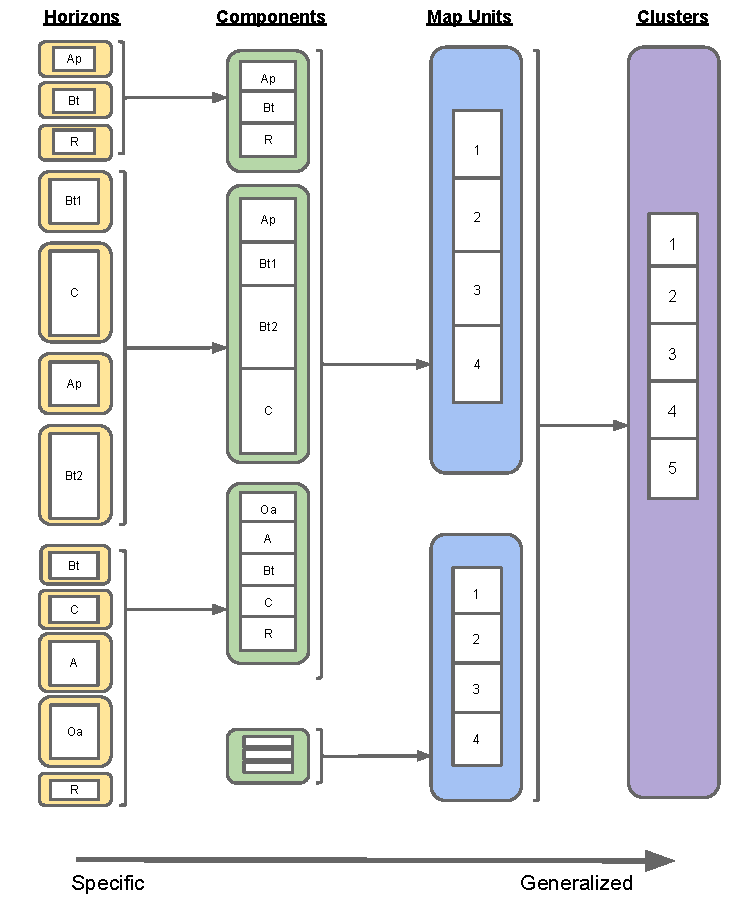
\includegraphics[width=0.8\textwidth]{./img/aggregation_flow_diagram}
	\caption[Flow diagram of the soil aggregation process]{Flow diagram of the soil aggregation process. Horizons are grouped together according to which component they belong. Components are grouped together according to which map unit they  belong. A weighted average is calculated, based upon the component percentage. Mapunits are grouped together according to hydrologic soil group  and are then assigned to a cluster based on a clustering algorithm. Clusters are created by aggregated map units together using a depth-weighted average of soil properties for each horizon.}
	\label{fig:agg_flow_diagram}
\end{figure}

%%% SSURGO data structure
\begin{figure}[h]
\centering
 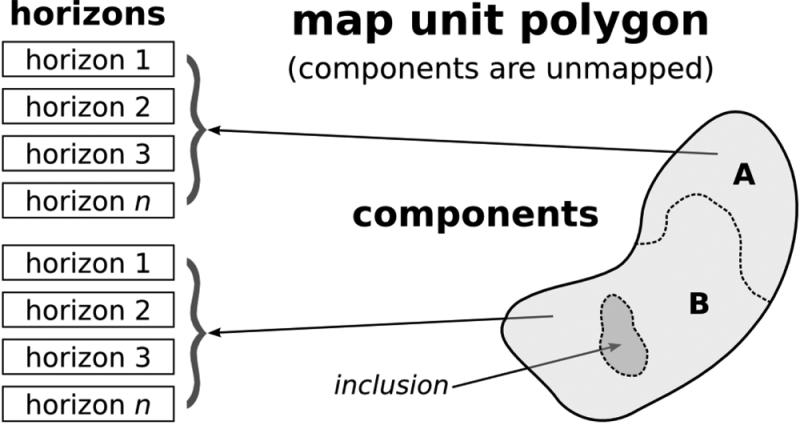
\includegraphics[width=0.5\textwidth]{./img/ssurgo_data_structure_schematic.jpeg}
	\caption[Schematic diagram of SSURGO data structure]{Schematic diagram of SSURGO data structure \cite{gatzke_aggregation_2011}}.
	\label{fig:ssurgo_schematic}
\end{figure}

%% SSURGO profile figures
\begin{figure}[h]
  \centering
    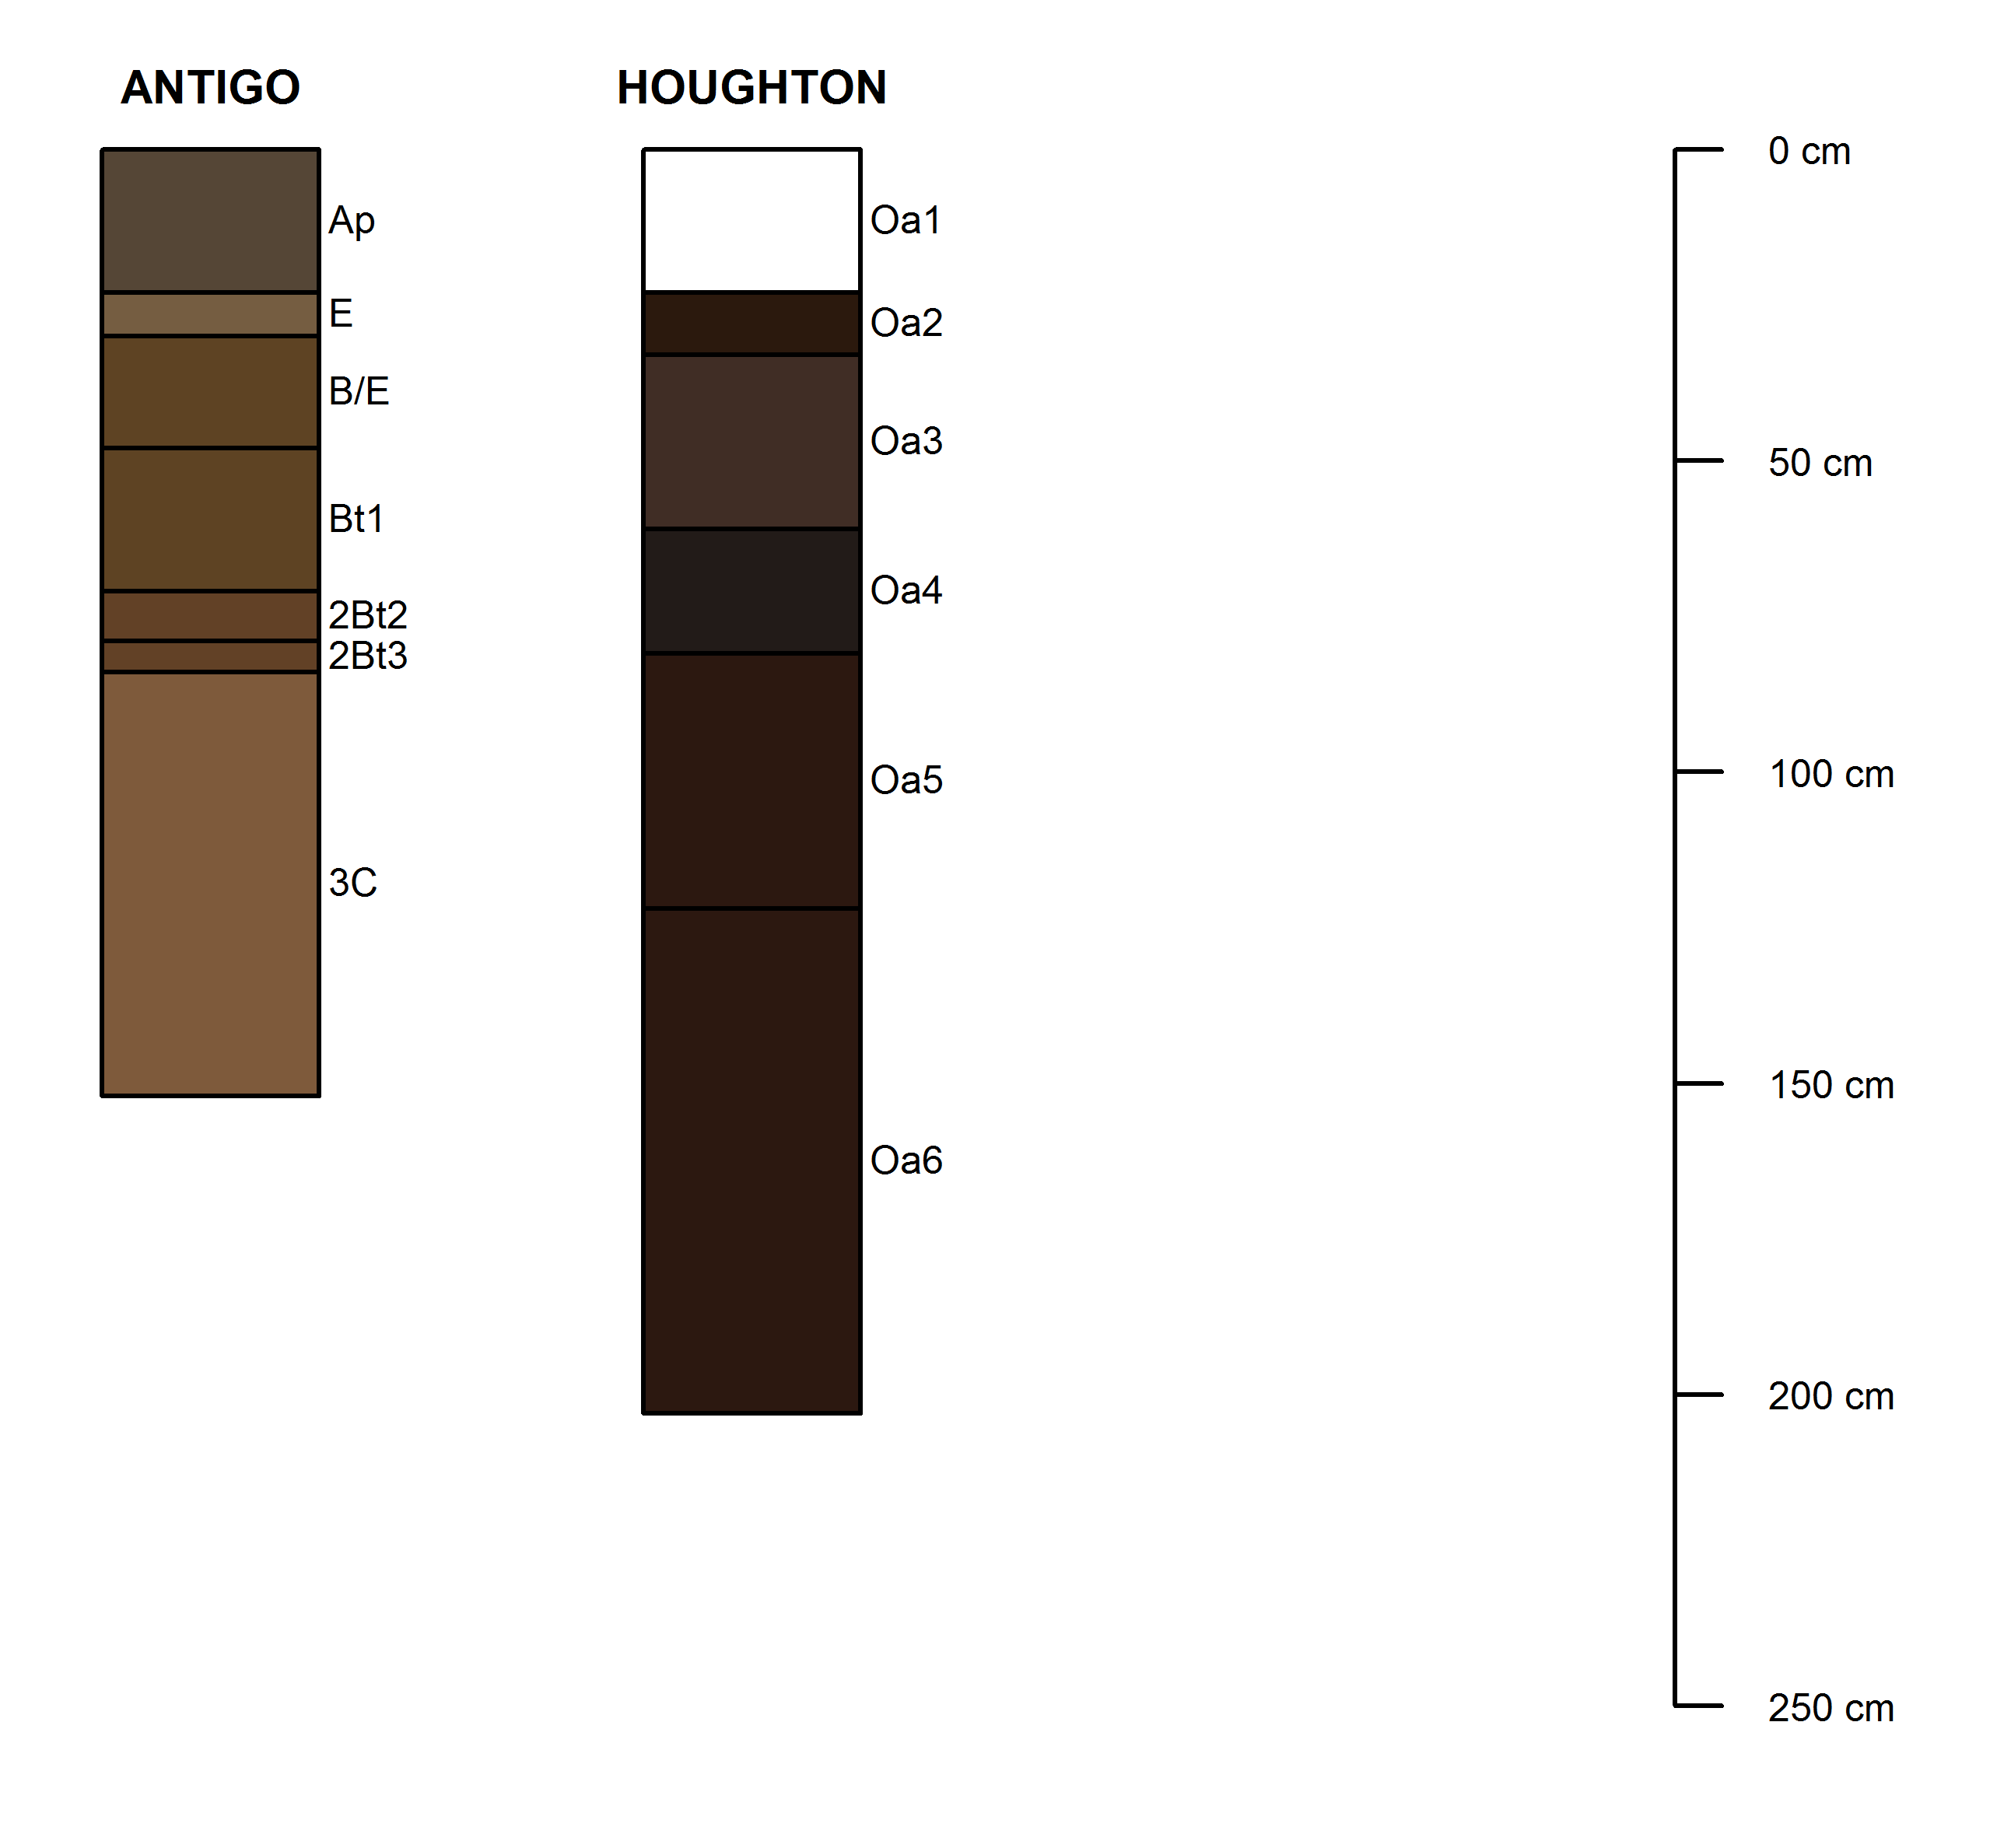
\includegraphics[width=0.5\textwidth]{./img/component_schematic.png}
	\caption[Schematic diagram of SSURGO map unit]{Schematic diagram of SSURGO map unit. Antigo and Houghton are each components within the map unit. Within each map unit are varying numbers of components with varying horizon depths (e.g., Ap and O1 are the surface horizons for Antigo and Houghton respectively. Components were aggregated to map units by averaging soil properties (e.g., percent sand) horizontally across horizons.}
	\label{fig:component_schematic}
\end{figure}
%%Soil cluster variability
\clearpage
\begin{figure}[H]
	\centering
	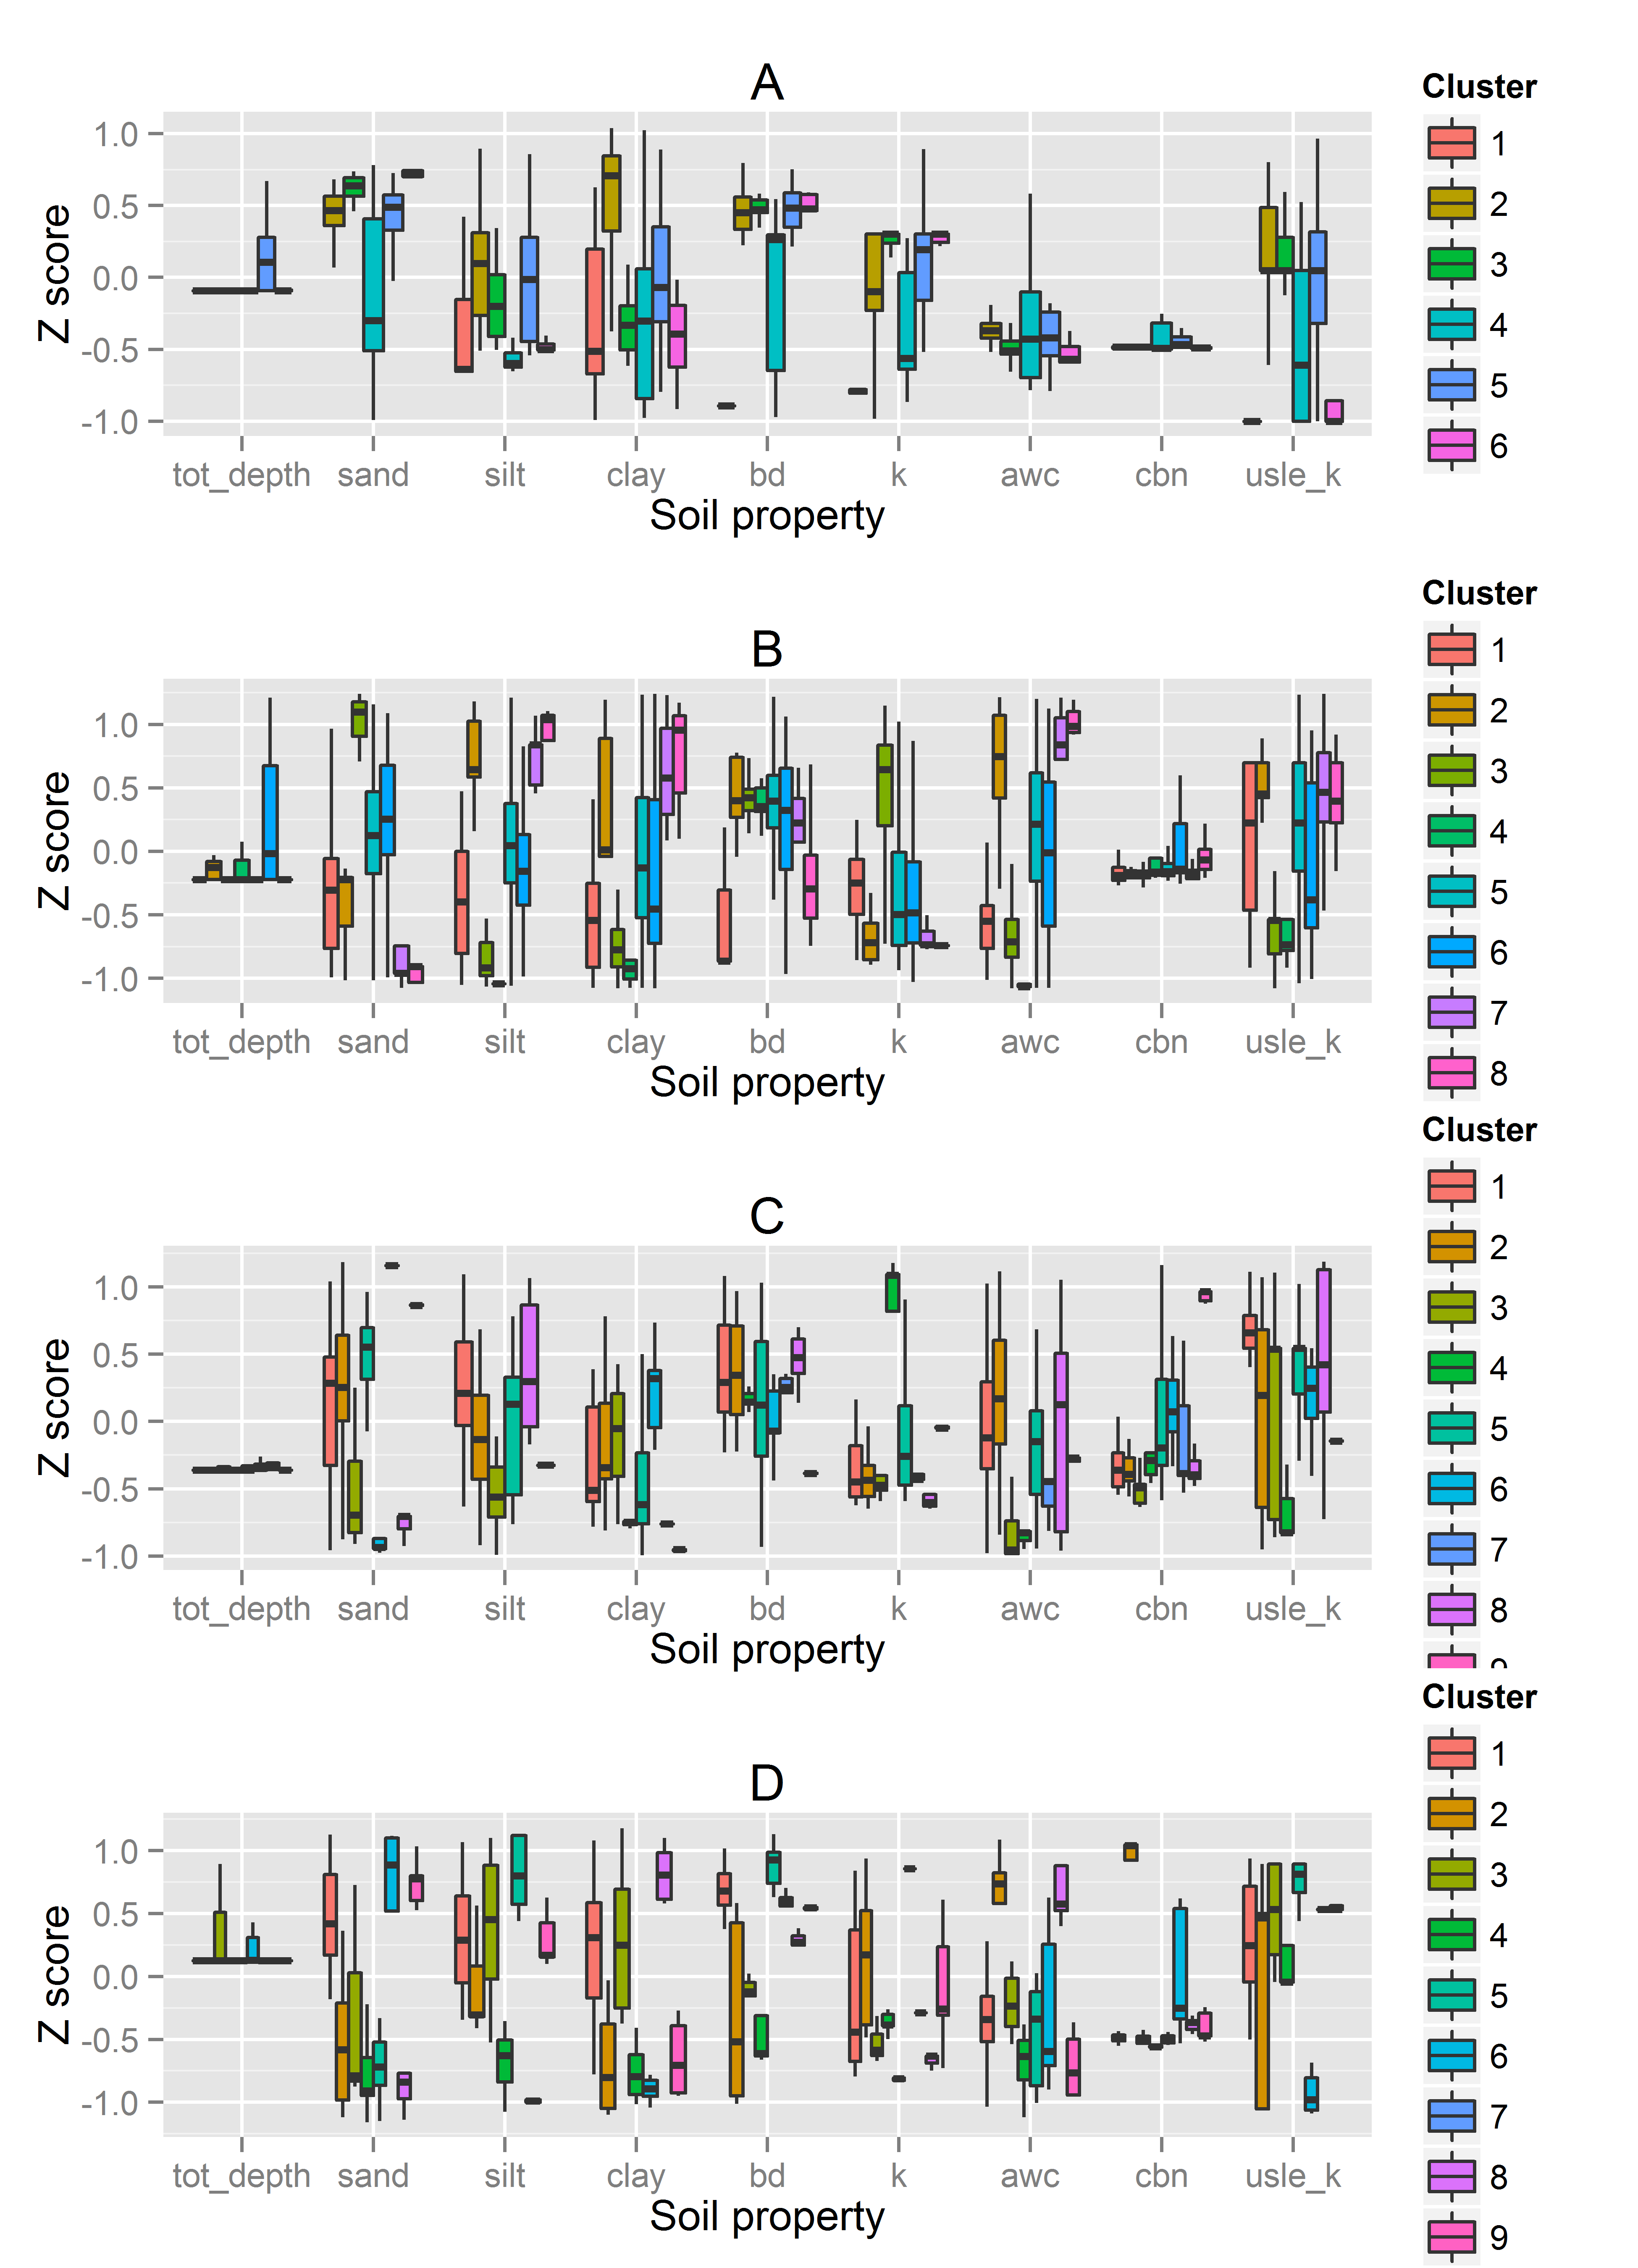
\includegraphics[width=\textwidth]{./img/cluster_variability.png}
	\caption[Boxplots showing the variability of soil properties]{Boxplots showing the variability of soil properties within the final set of soil clusters. The letter above each plot denotes hydrologic soil group (HSG). Each color represents a cluster of map units. The Z score for each soil property is reported as $Z = X - \mu / \sigma$ where $X$ is the value of the soil property, $\mu$ and $\sigma$ are the population mean and standard deviation of a soil property. Outliers were excluded. The x-axis shows soil properties where tot\_depth is the soil depth, sand/silt/clay are the percent composition of each texture class, bd is bulk density, k is saturated conductivity, awc is available water capacity, cbn is organic carbon concentration, and usle\_k is soil erodibility.}
	\label{fig:soil_boxplots}
\end{figure}

%%Precipitation
\begin{landscape}
\begin{figure}[h]

	\begin{tabular}{c c}
		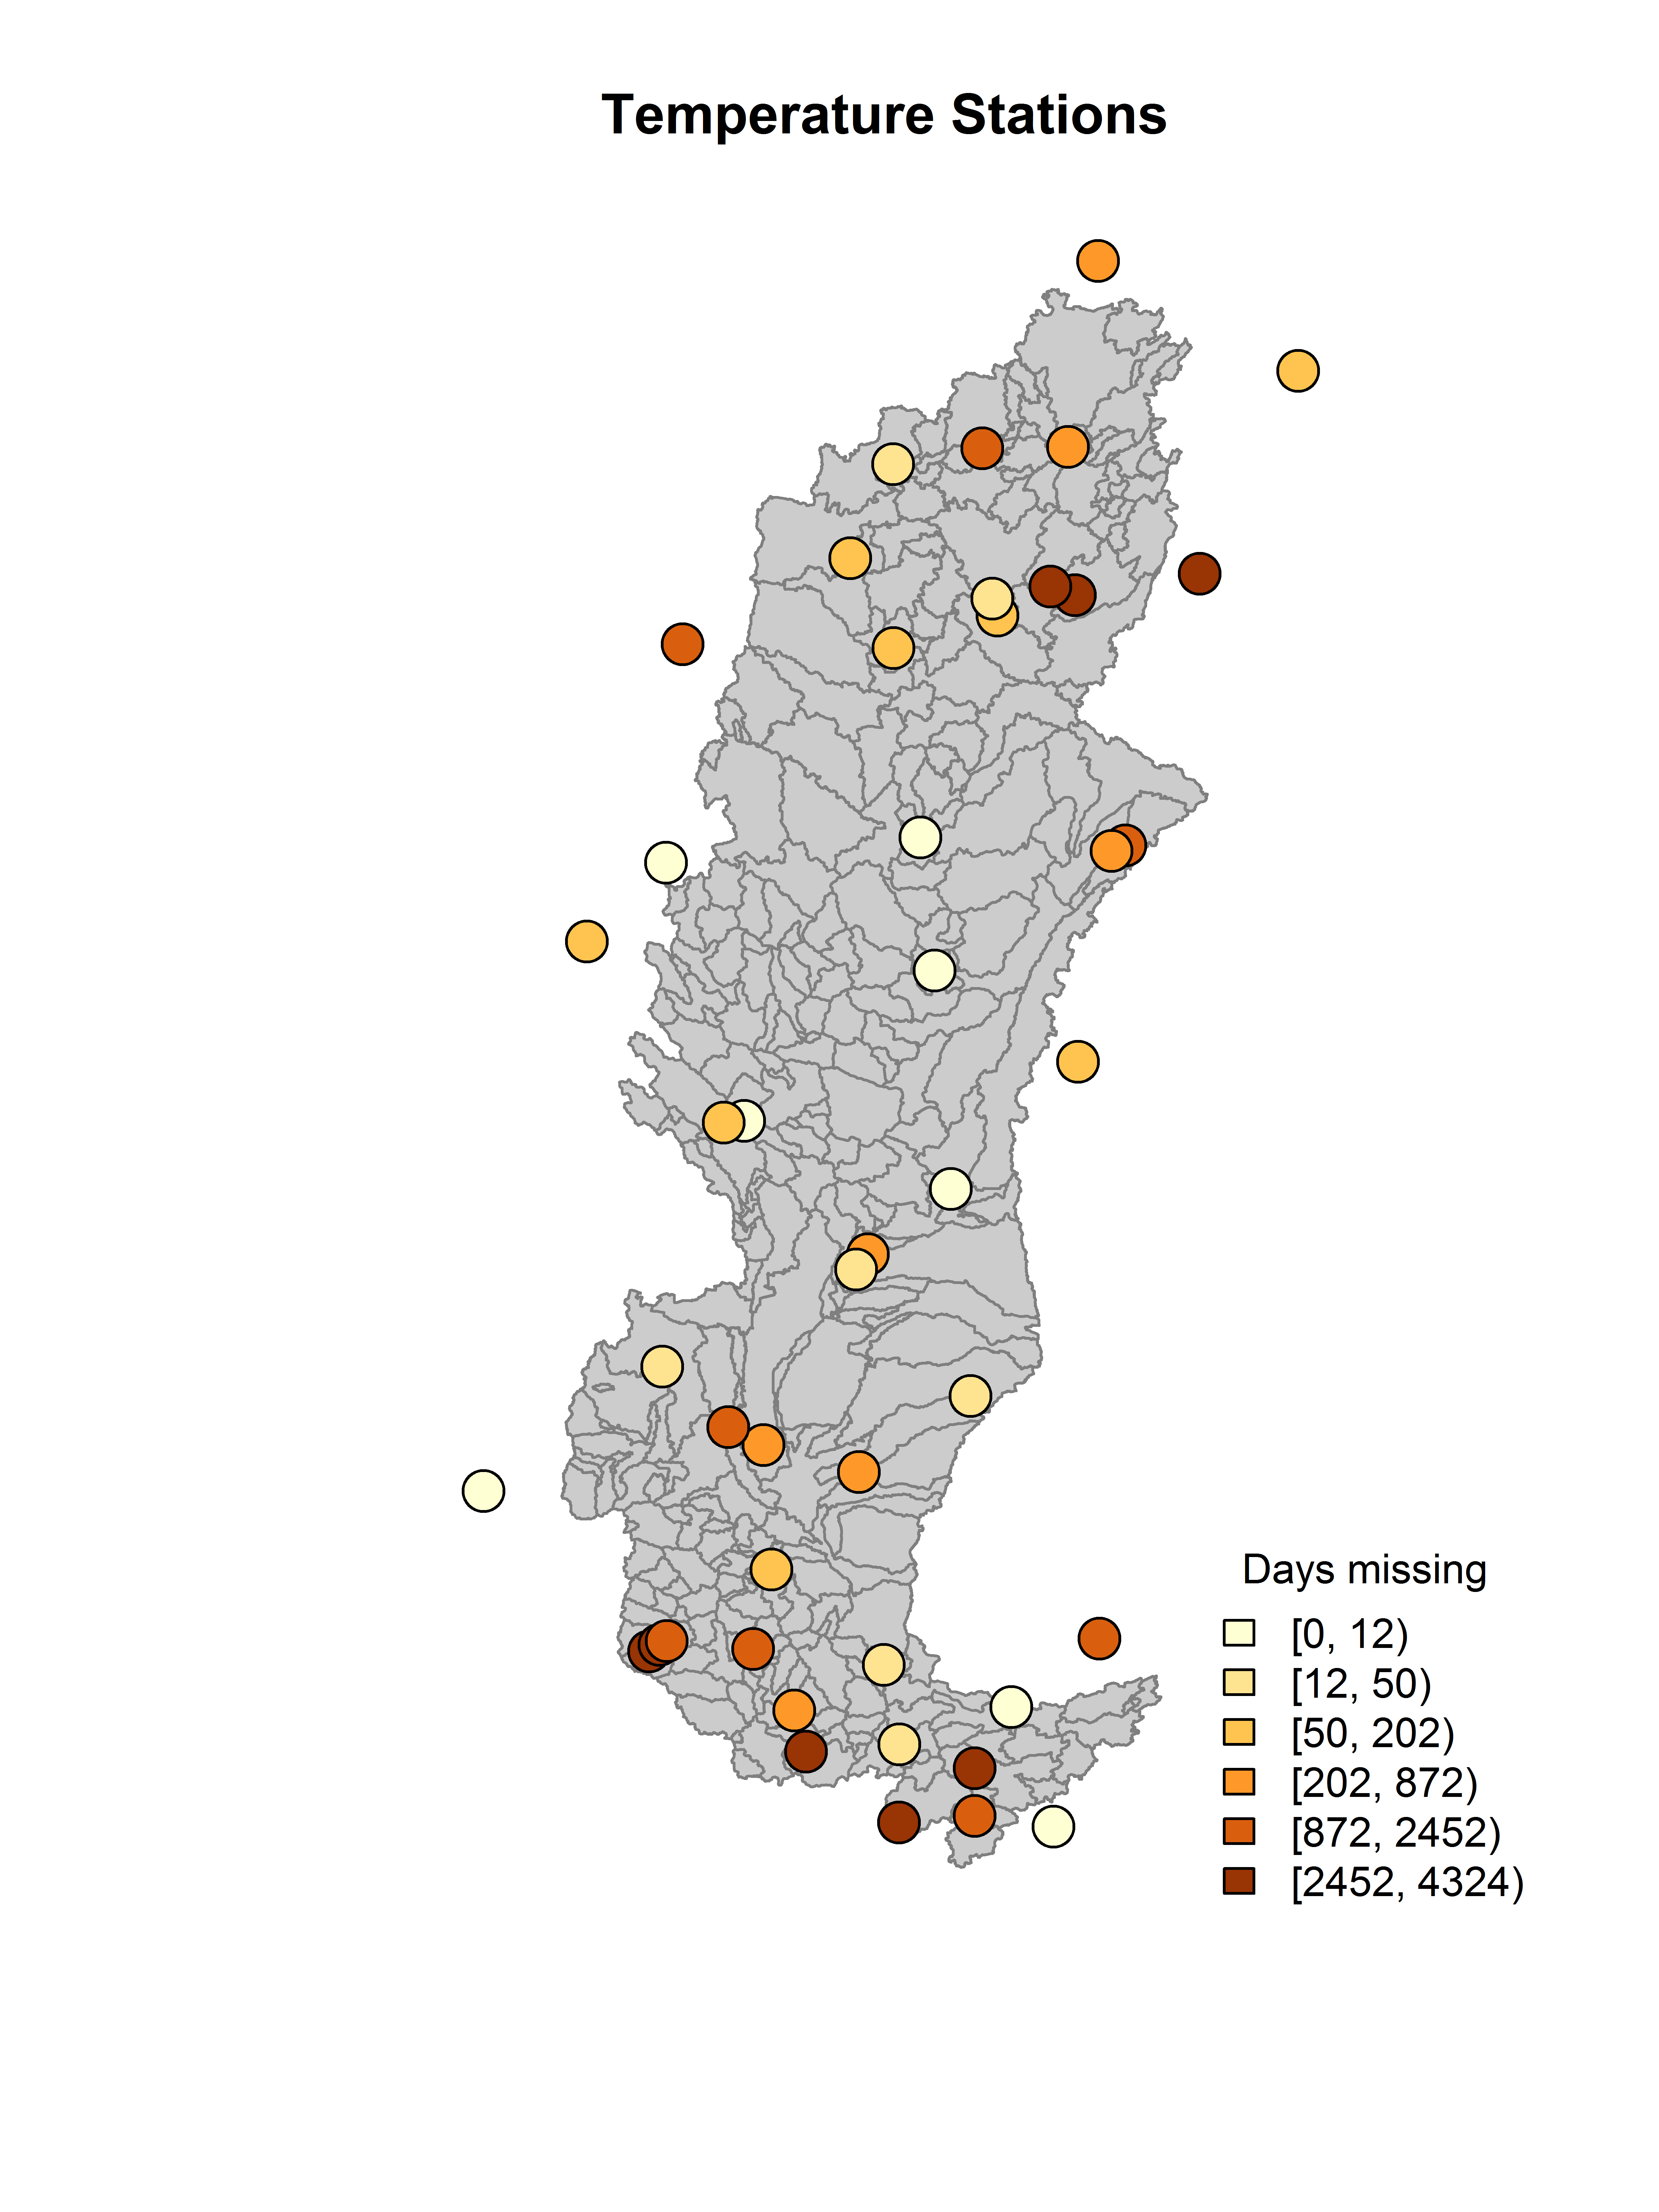
\includegraphics[scale = 0.5]{./img/tmp_na_counts} &	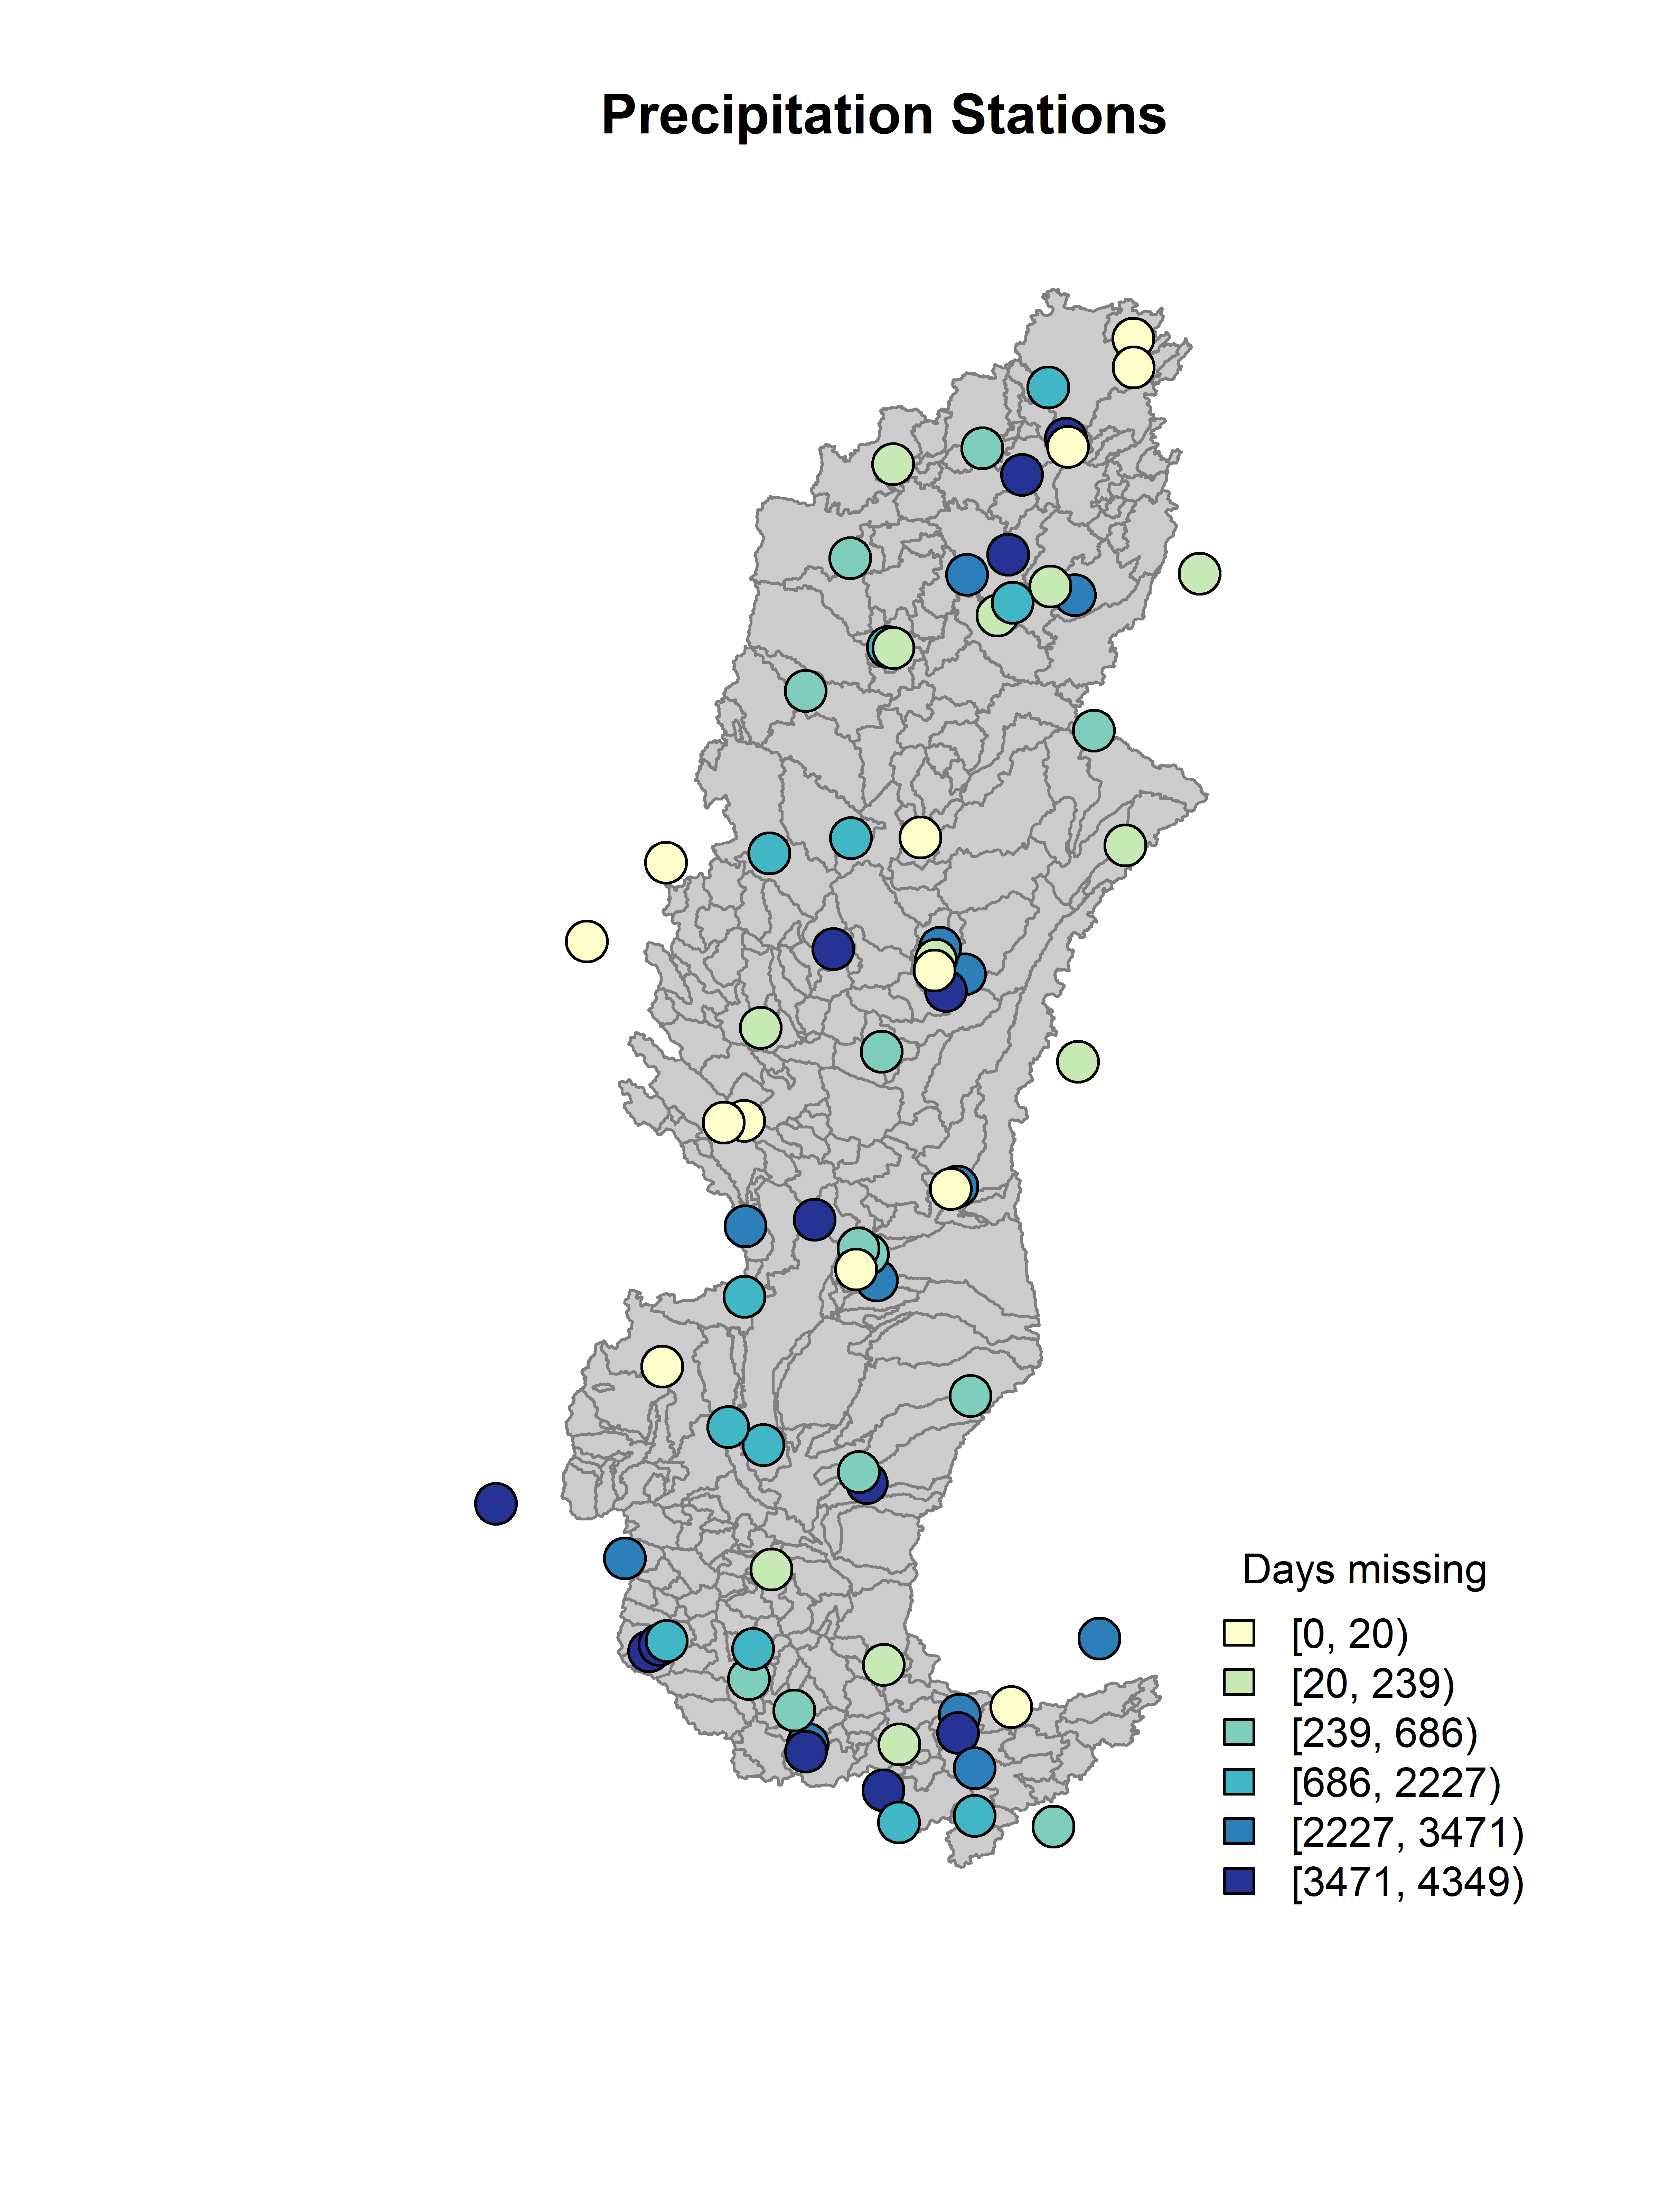
\includegraphics[scale=0.5]{./img/pcp_na_counts} \\
	\end{tabular}
	\caption{Maps displaying the climate stations used for in the SWAT model. Stations are colored according the number of days missing in the record.}
	\label{fig:climate_missing}

\end{figure}
\end{landscape}

%%% ET figures
% for the et figures, pbias on top (hargreaves, pen, priestly), and nash sut on bottom (ditto)

\begin{landscape}
\begin{figure}
	\begin{tabular}{c c c l} % left bottom right top
	
		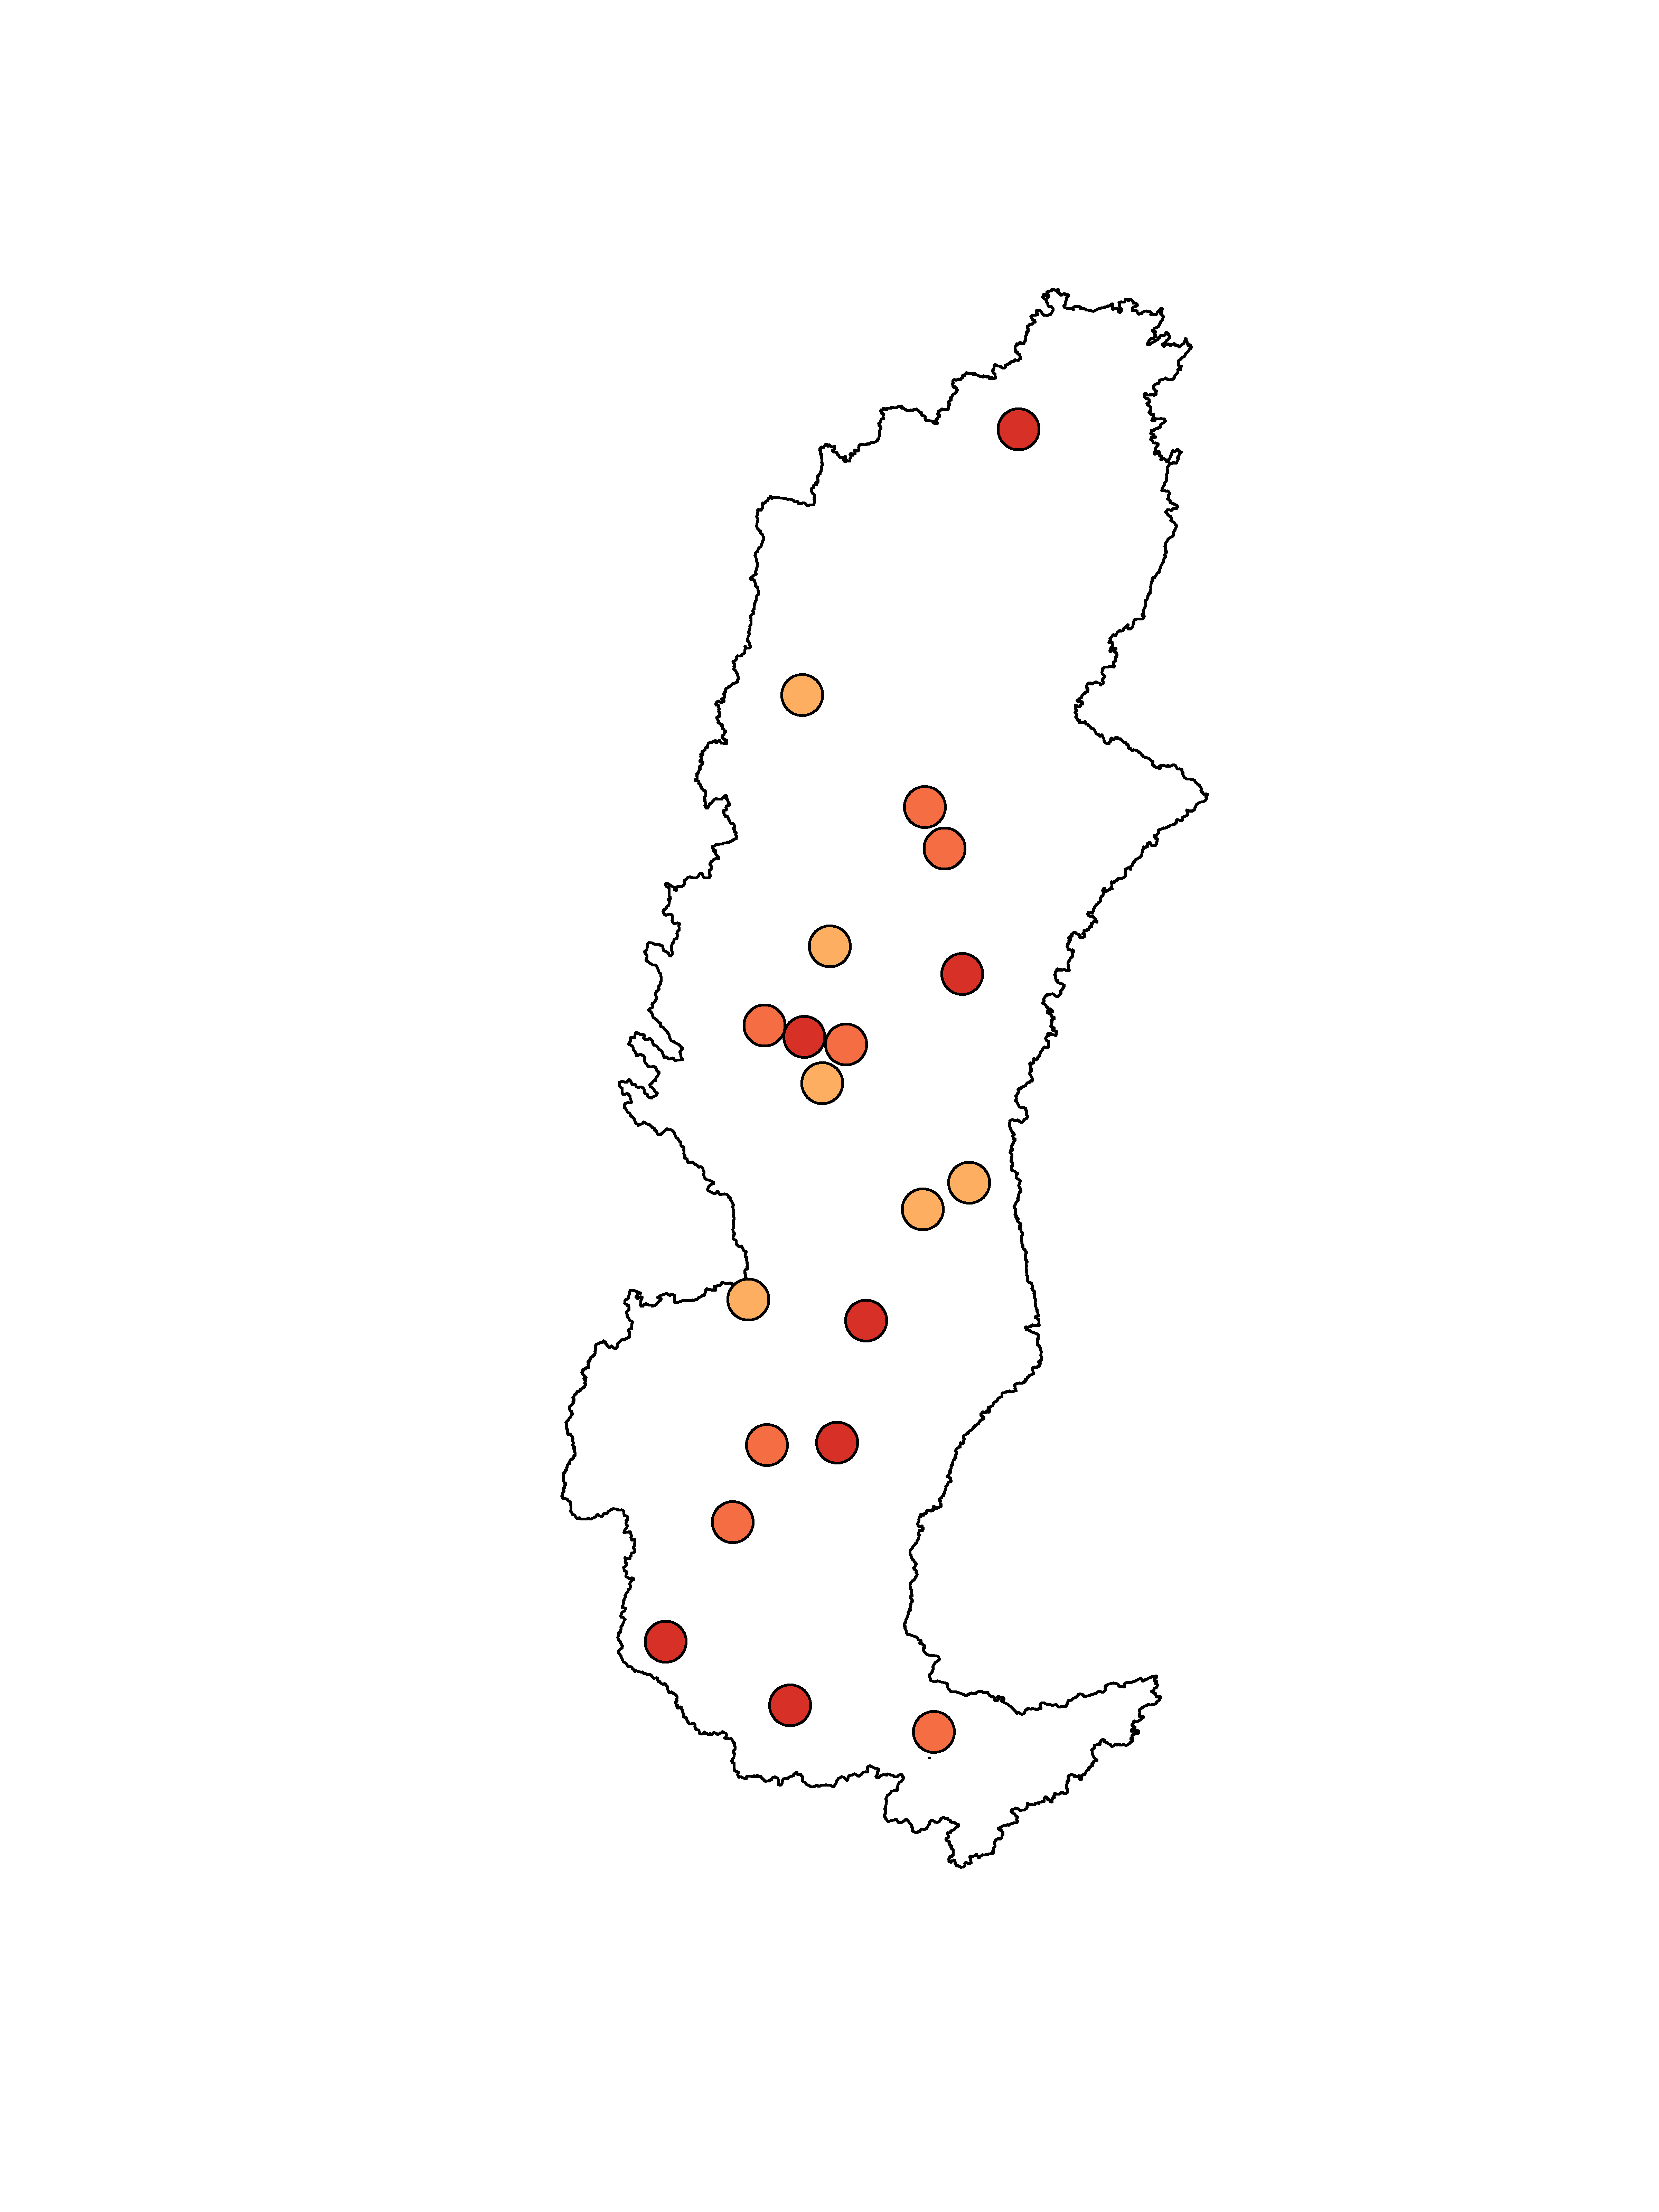
\includegraphics[trim= 4cm 2cm 1cm 2cm, clip, scale = 0.35]{./img/pbias_harg} &
			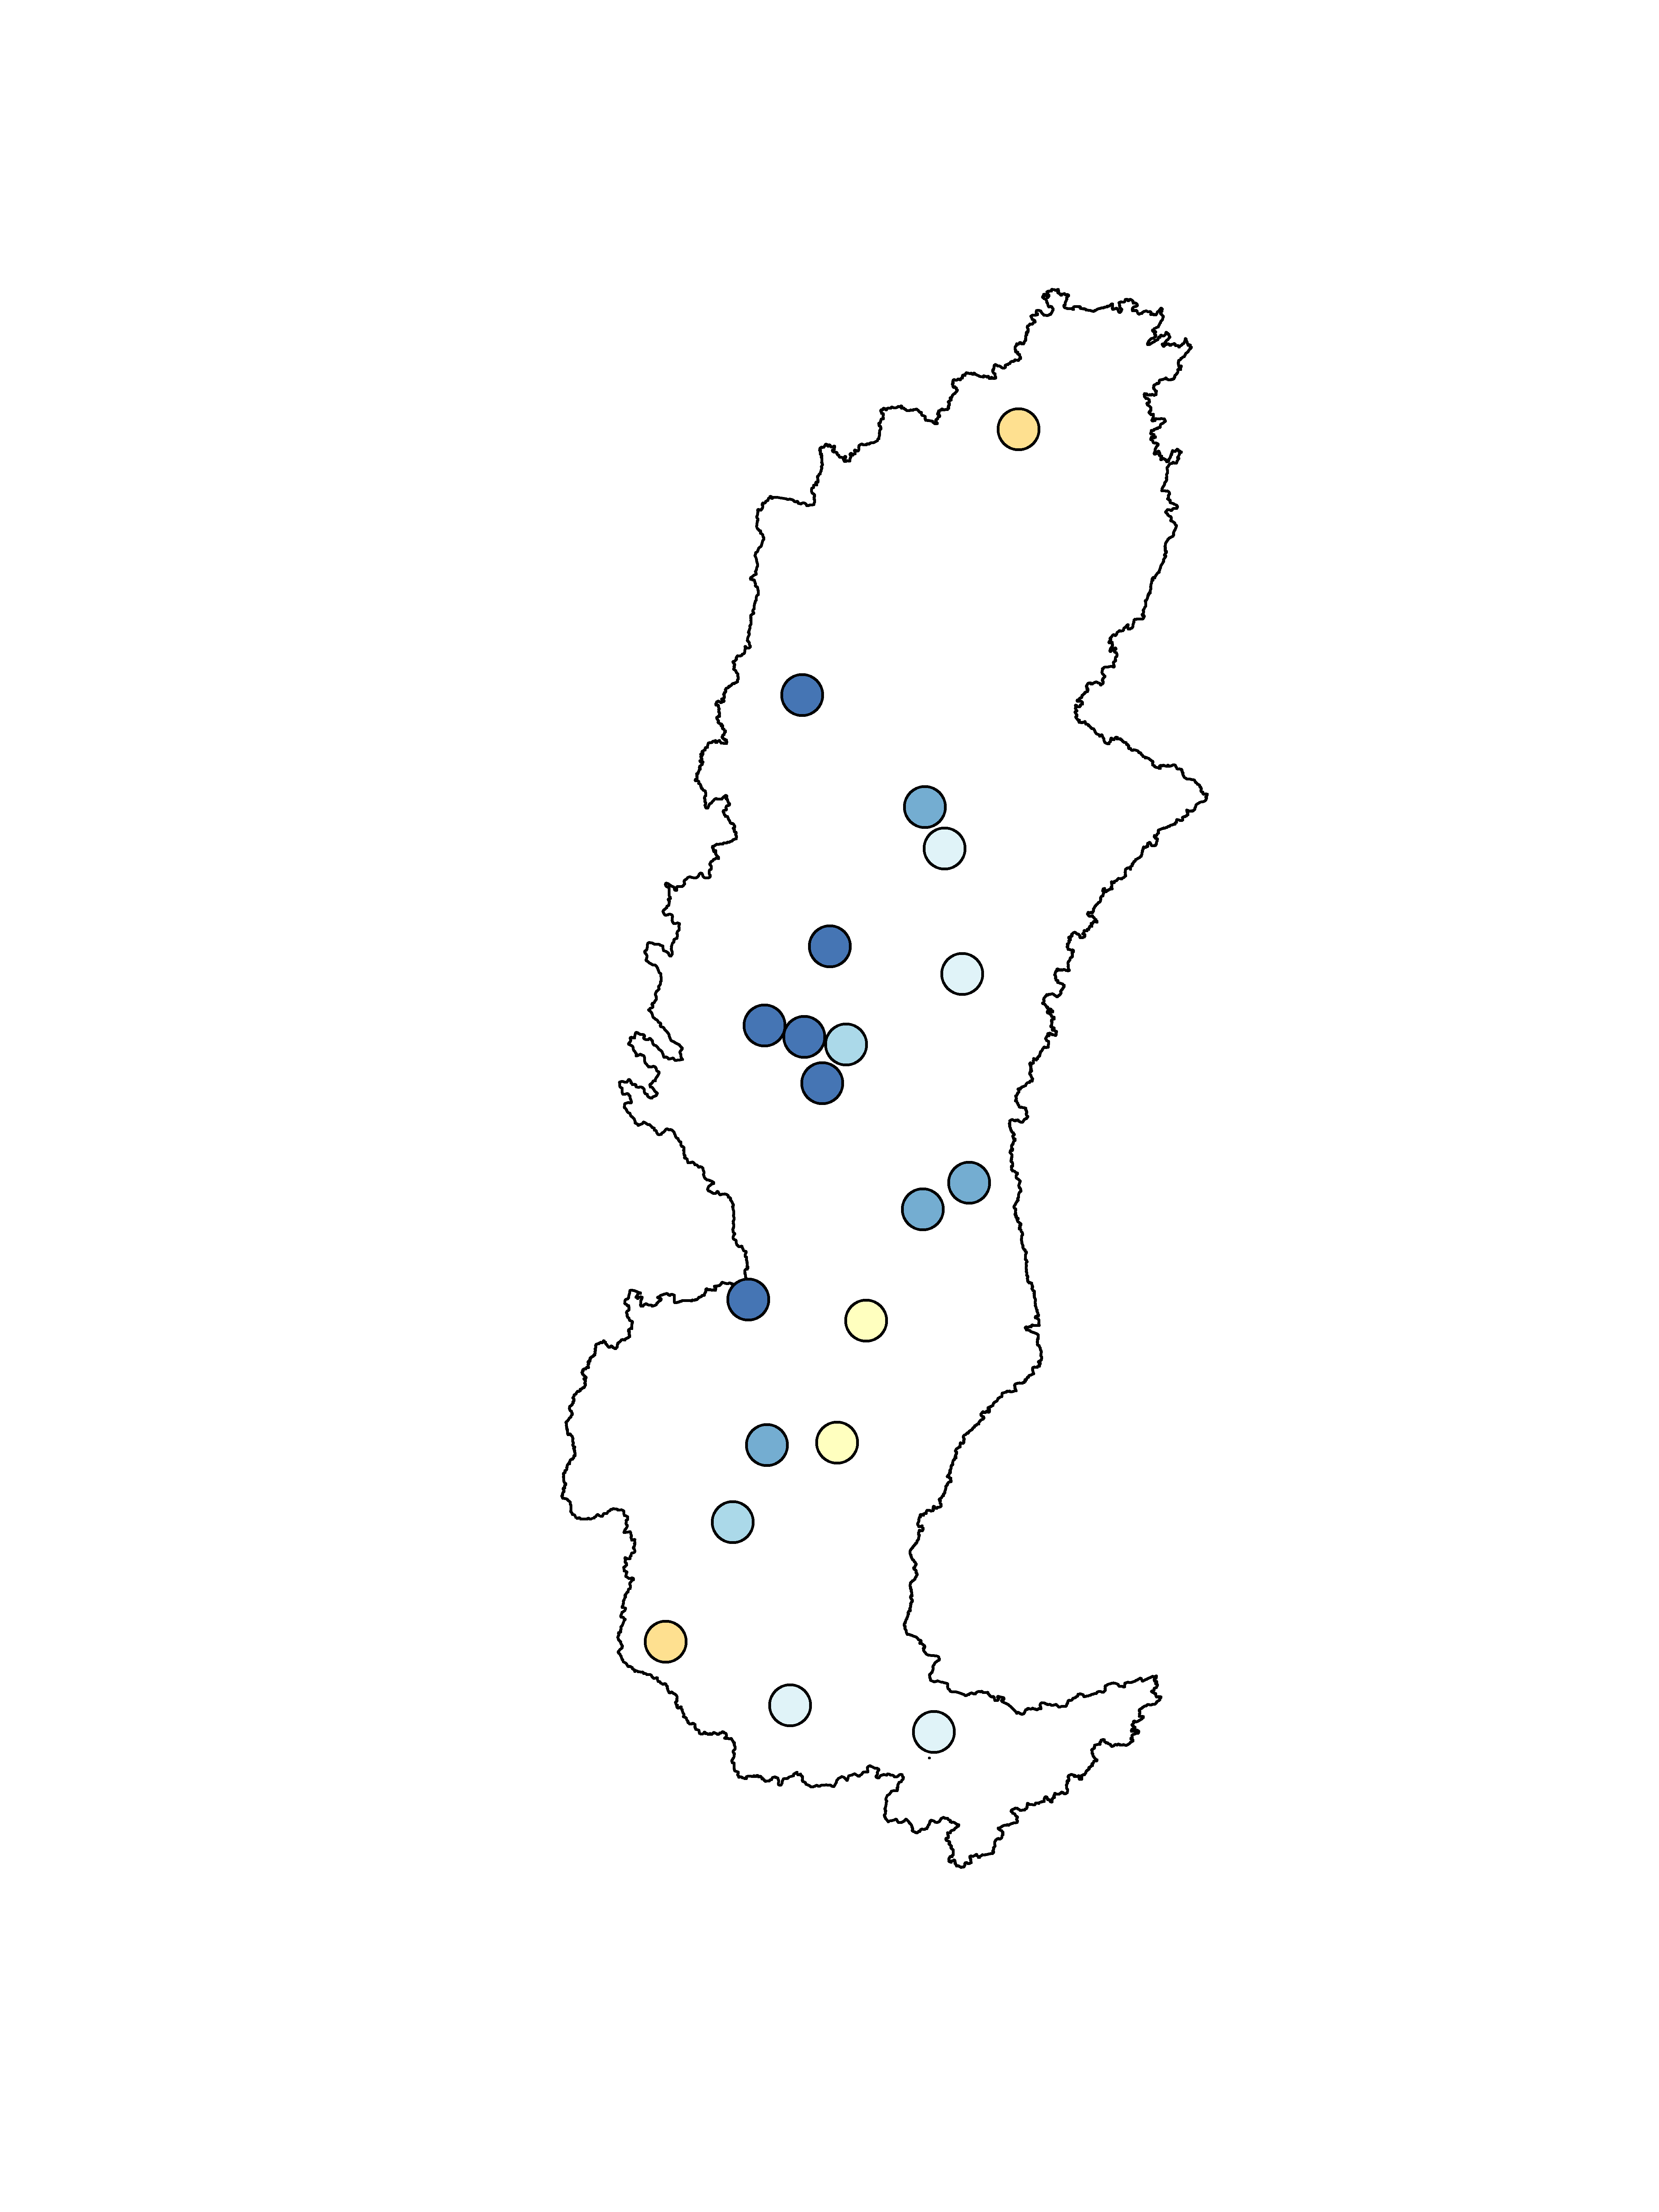
\includegraphics[trim= 4cm 2cm 1cm 2cm, clip, scale = 0.35]{./img/pbias_penman} &
				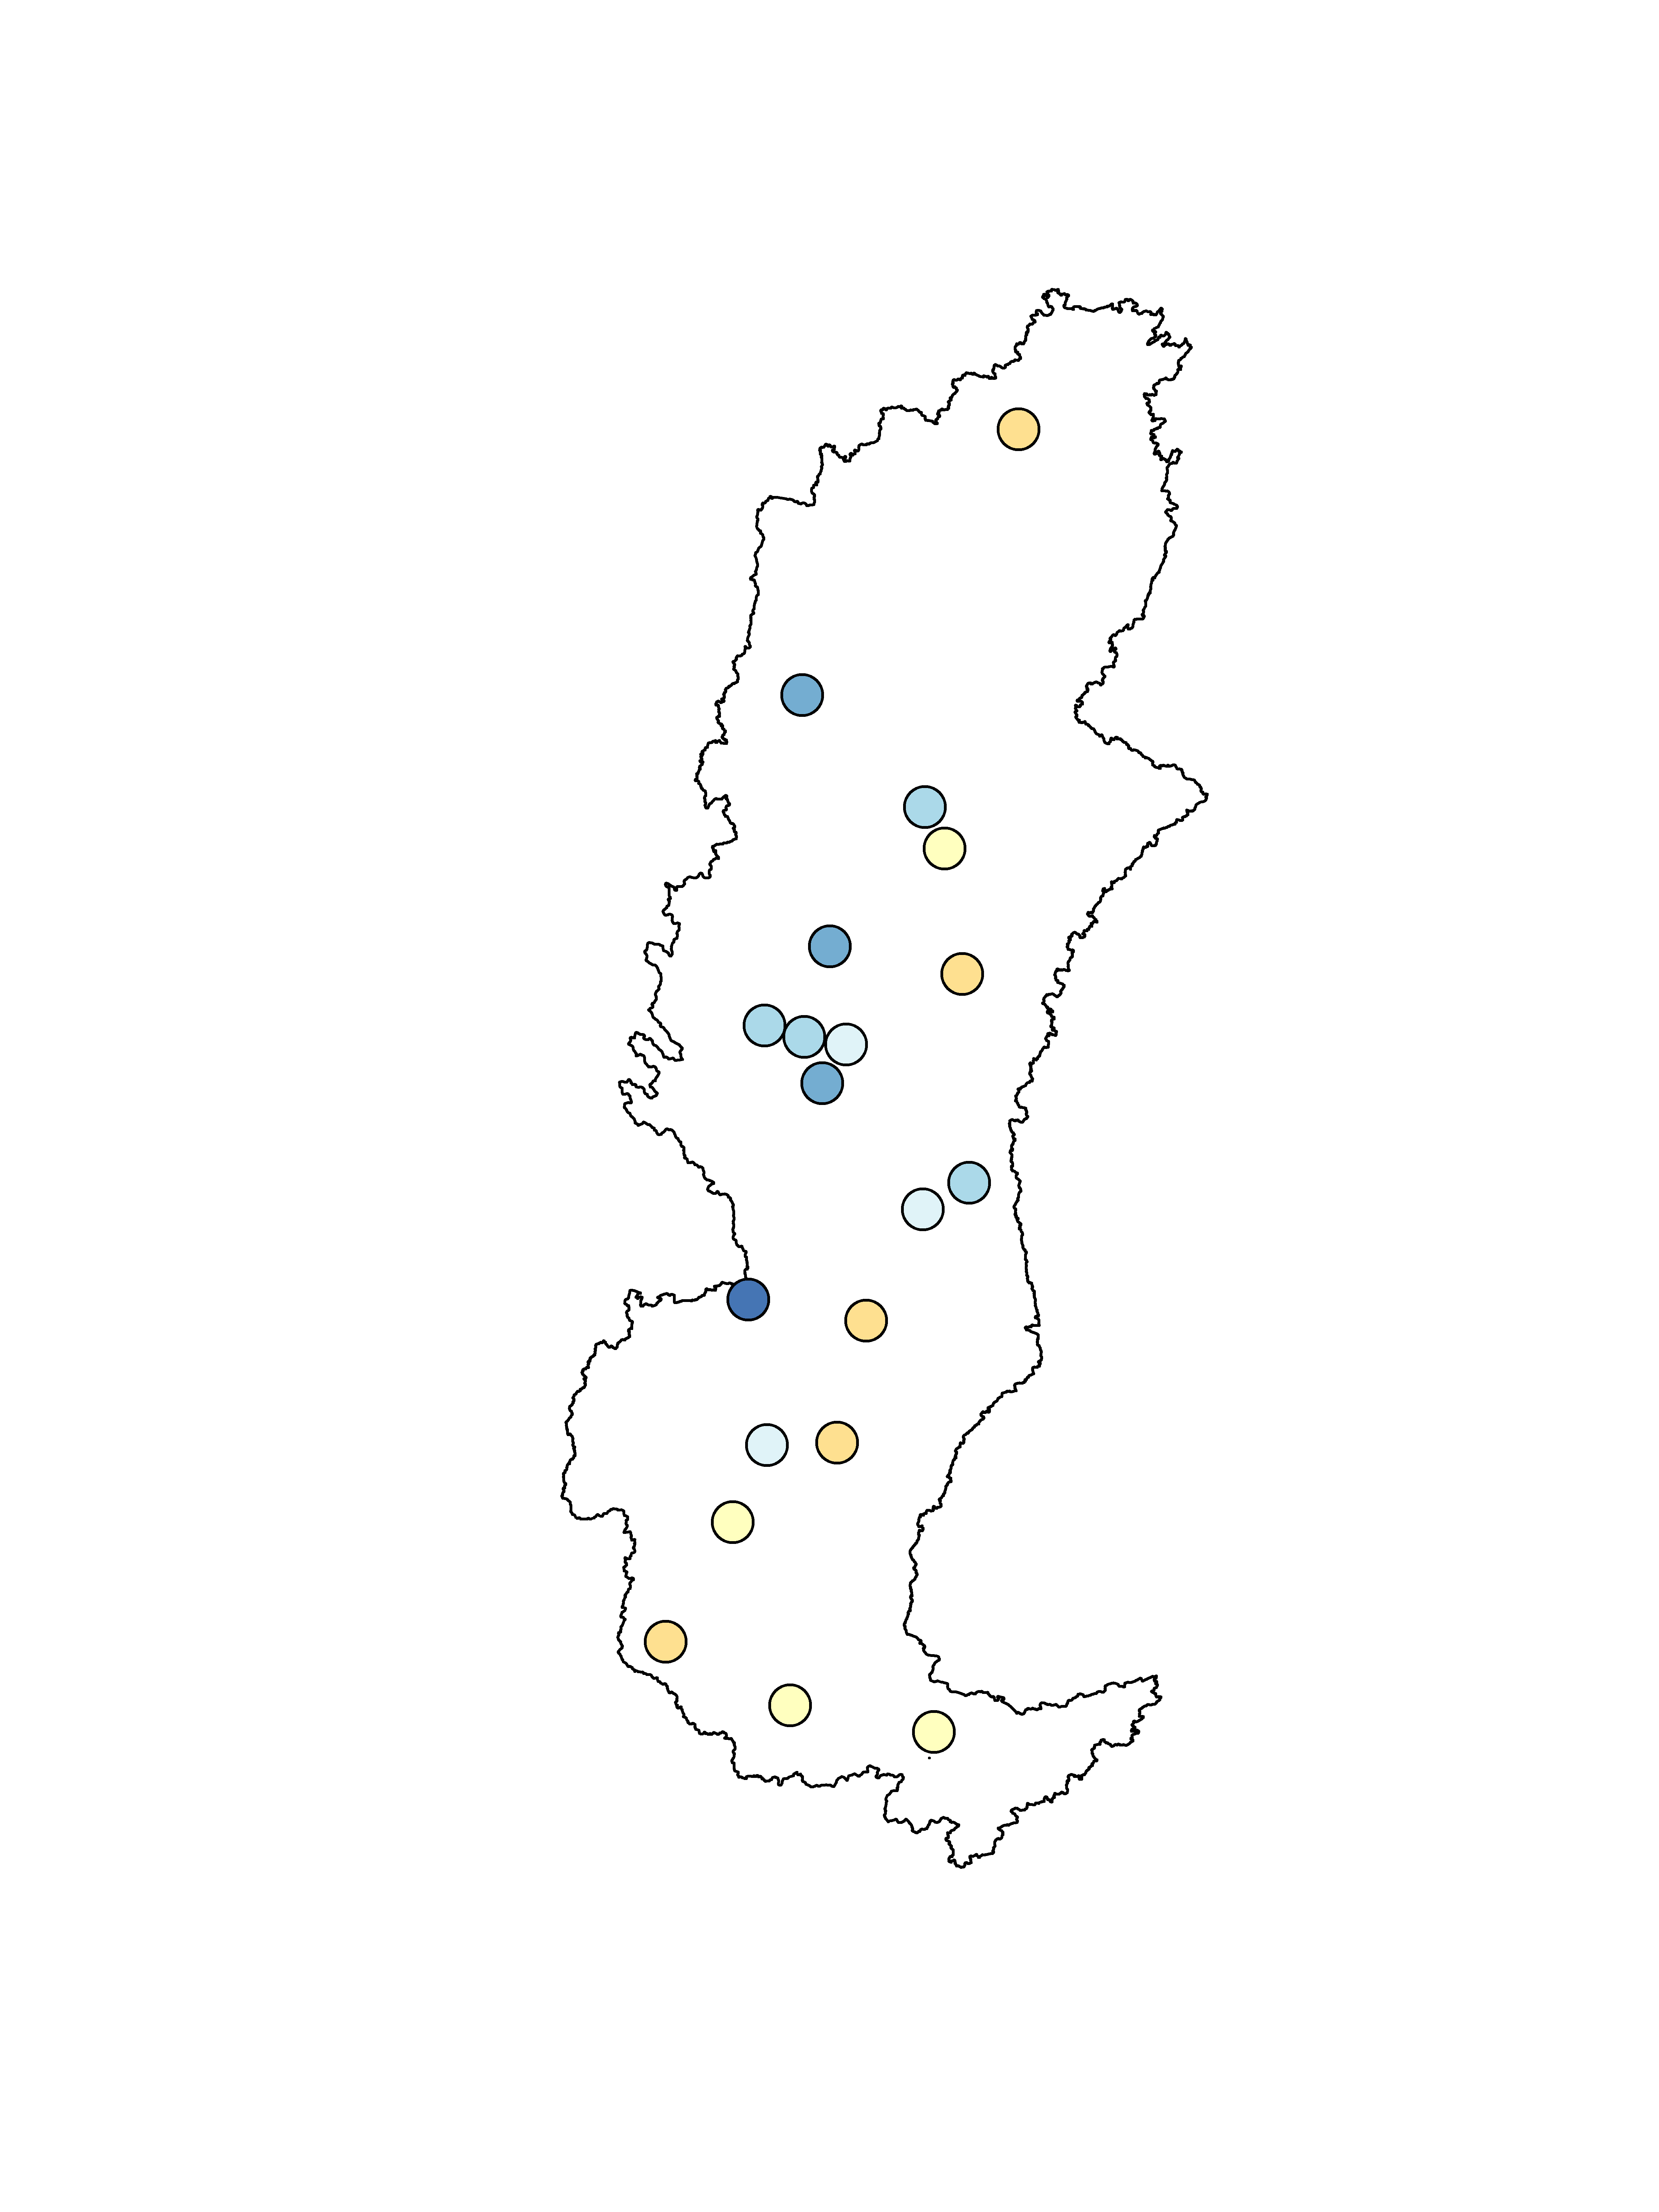
\includegraphics[trim= 4cm 2cm 1cm 2cm, clip, scale = 0.35]{./img/pbias_priestley} &
					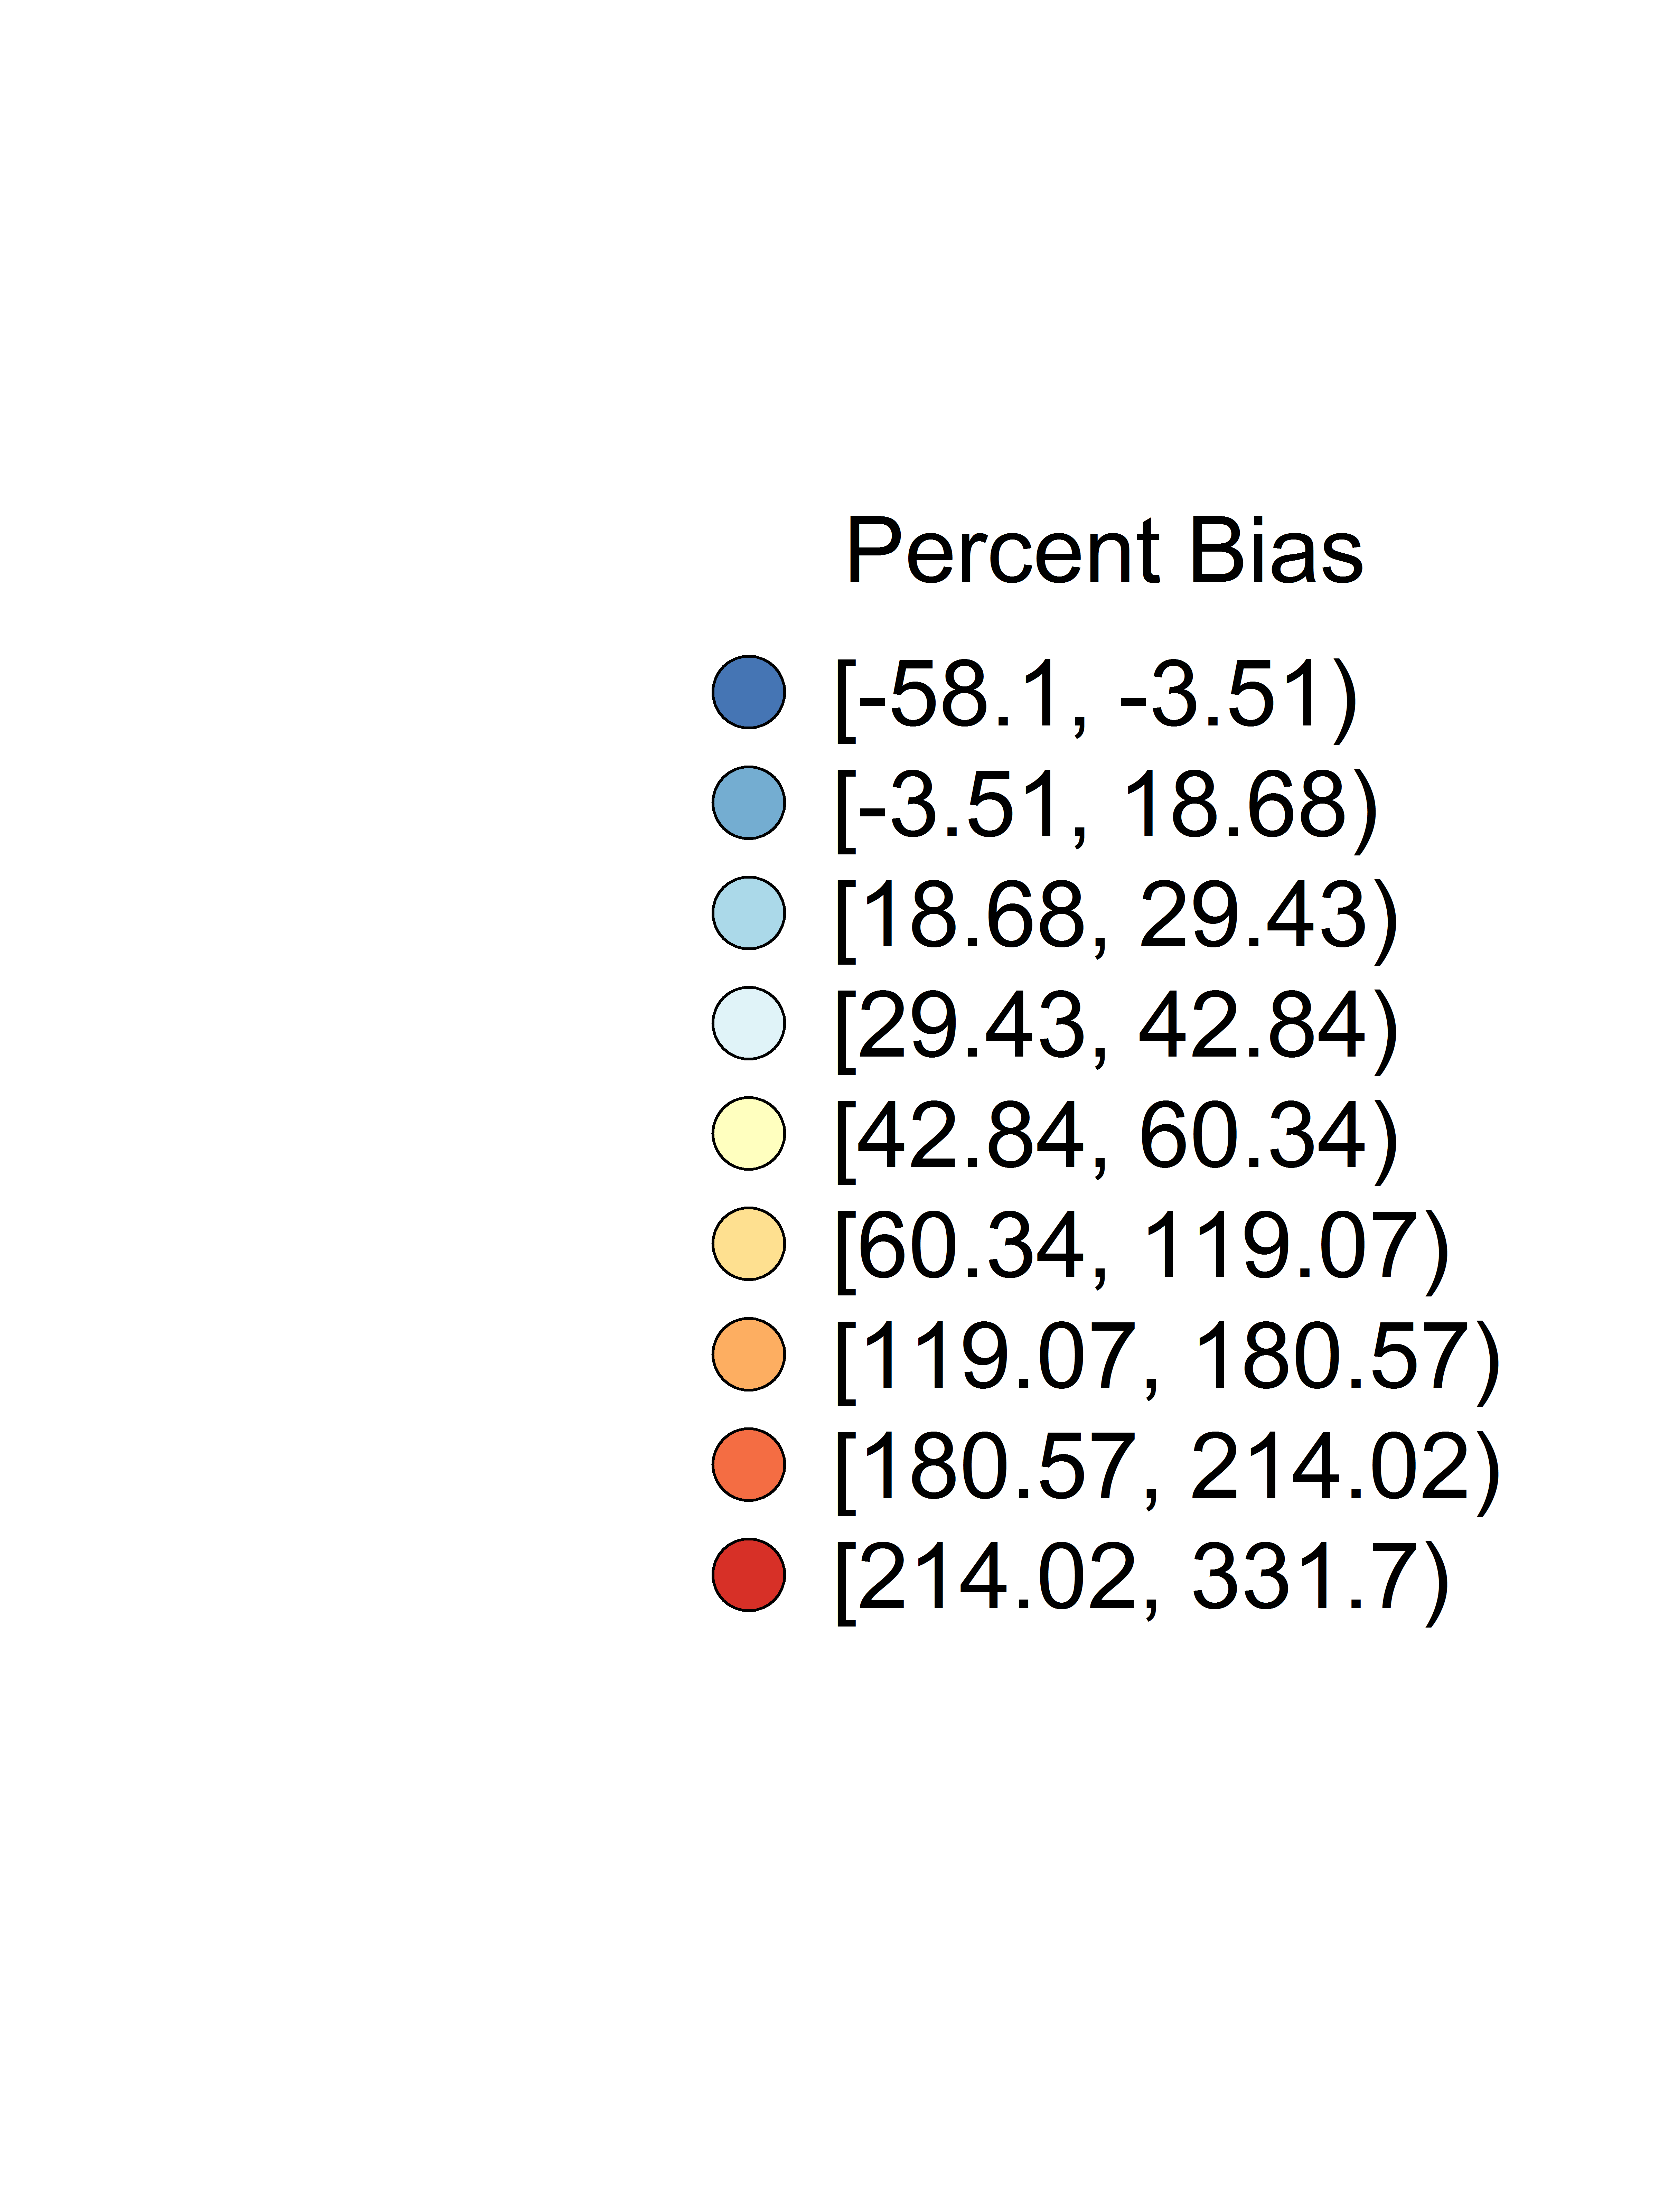
\includegraphics[trim= 5cm 2cm 0cm 3cm, clip, scale = 0.3]{./img/pbias_legend} \\
		{\bf Hargreaves} & {\bf Penman--Monteith} & {\bf Priestley--Taylor} & \\
		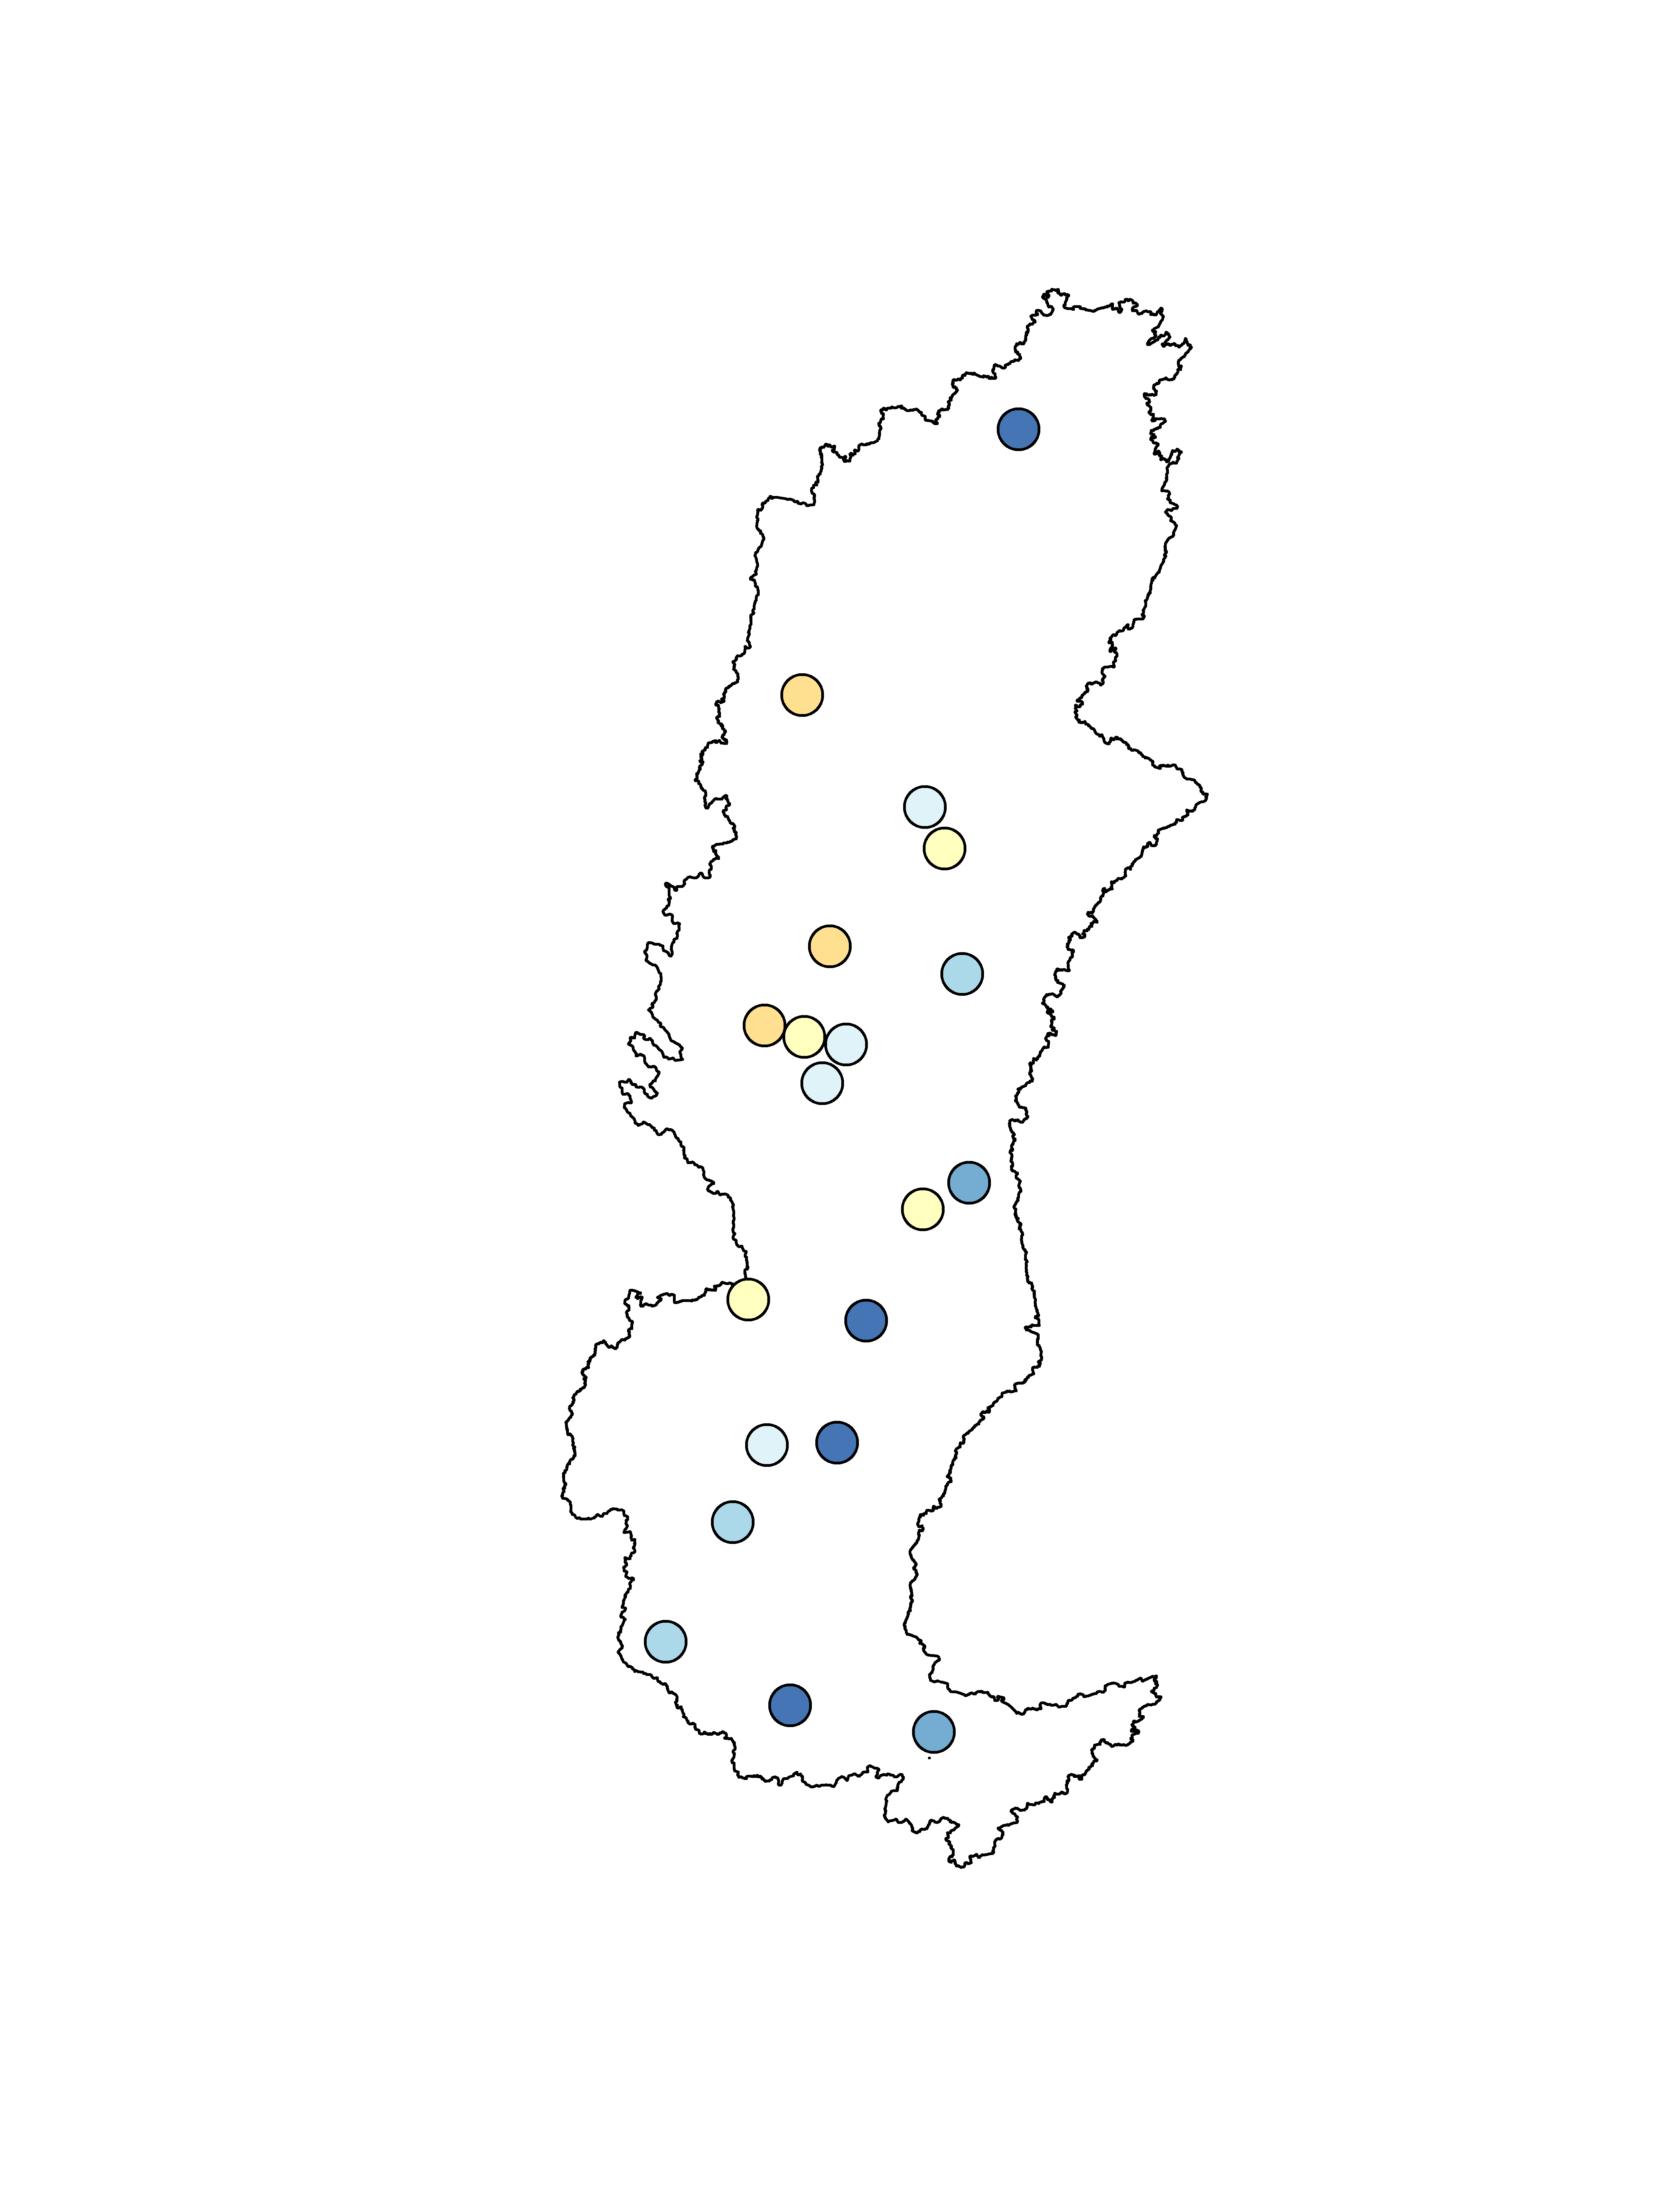
\includegraphics[trim= 4cm 2cm 1cm 2cm, clip, scale = 0.35]{./img/nashsut_harg} &
			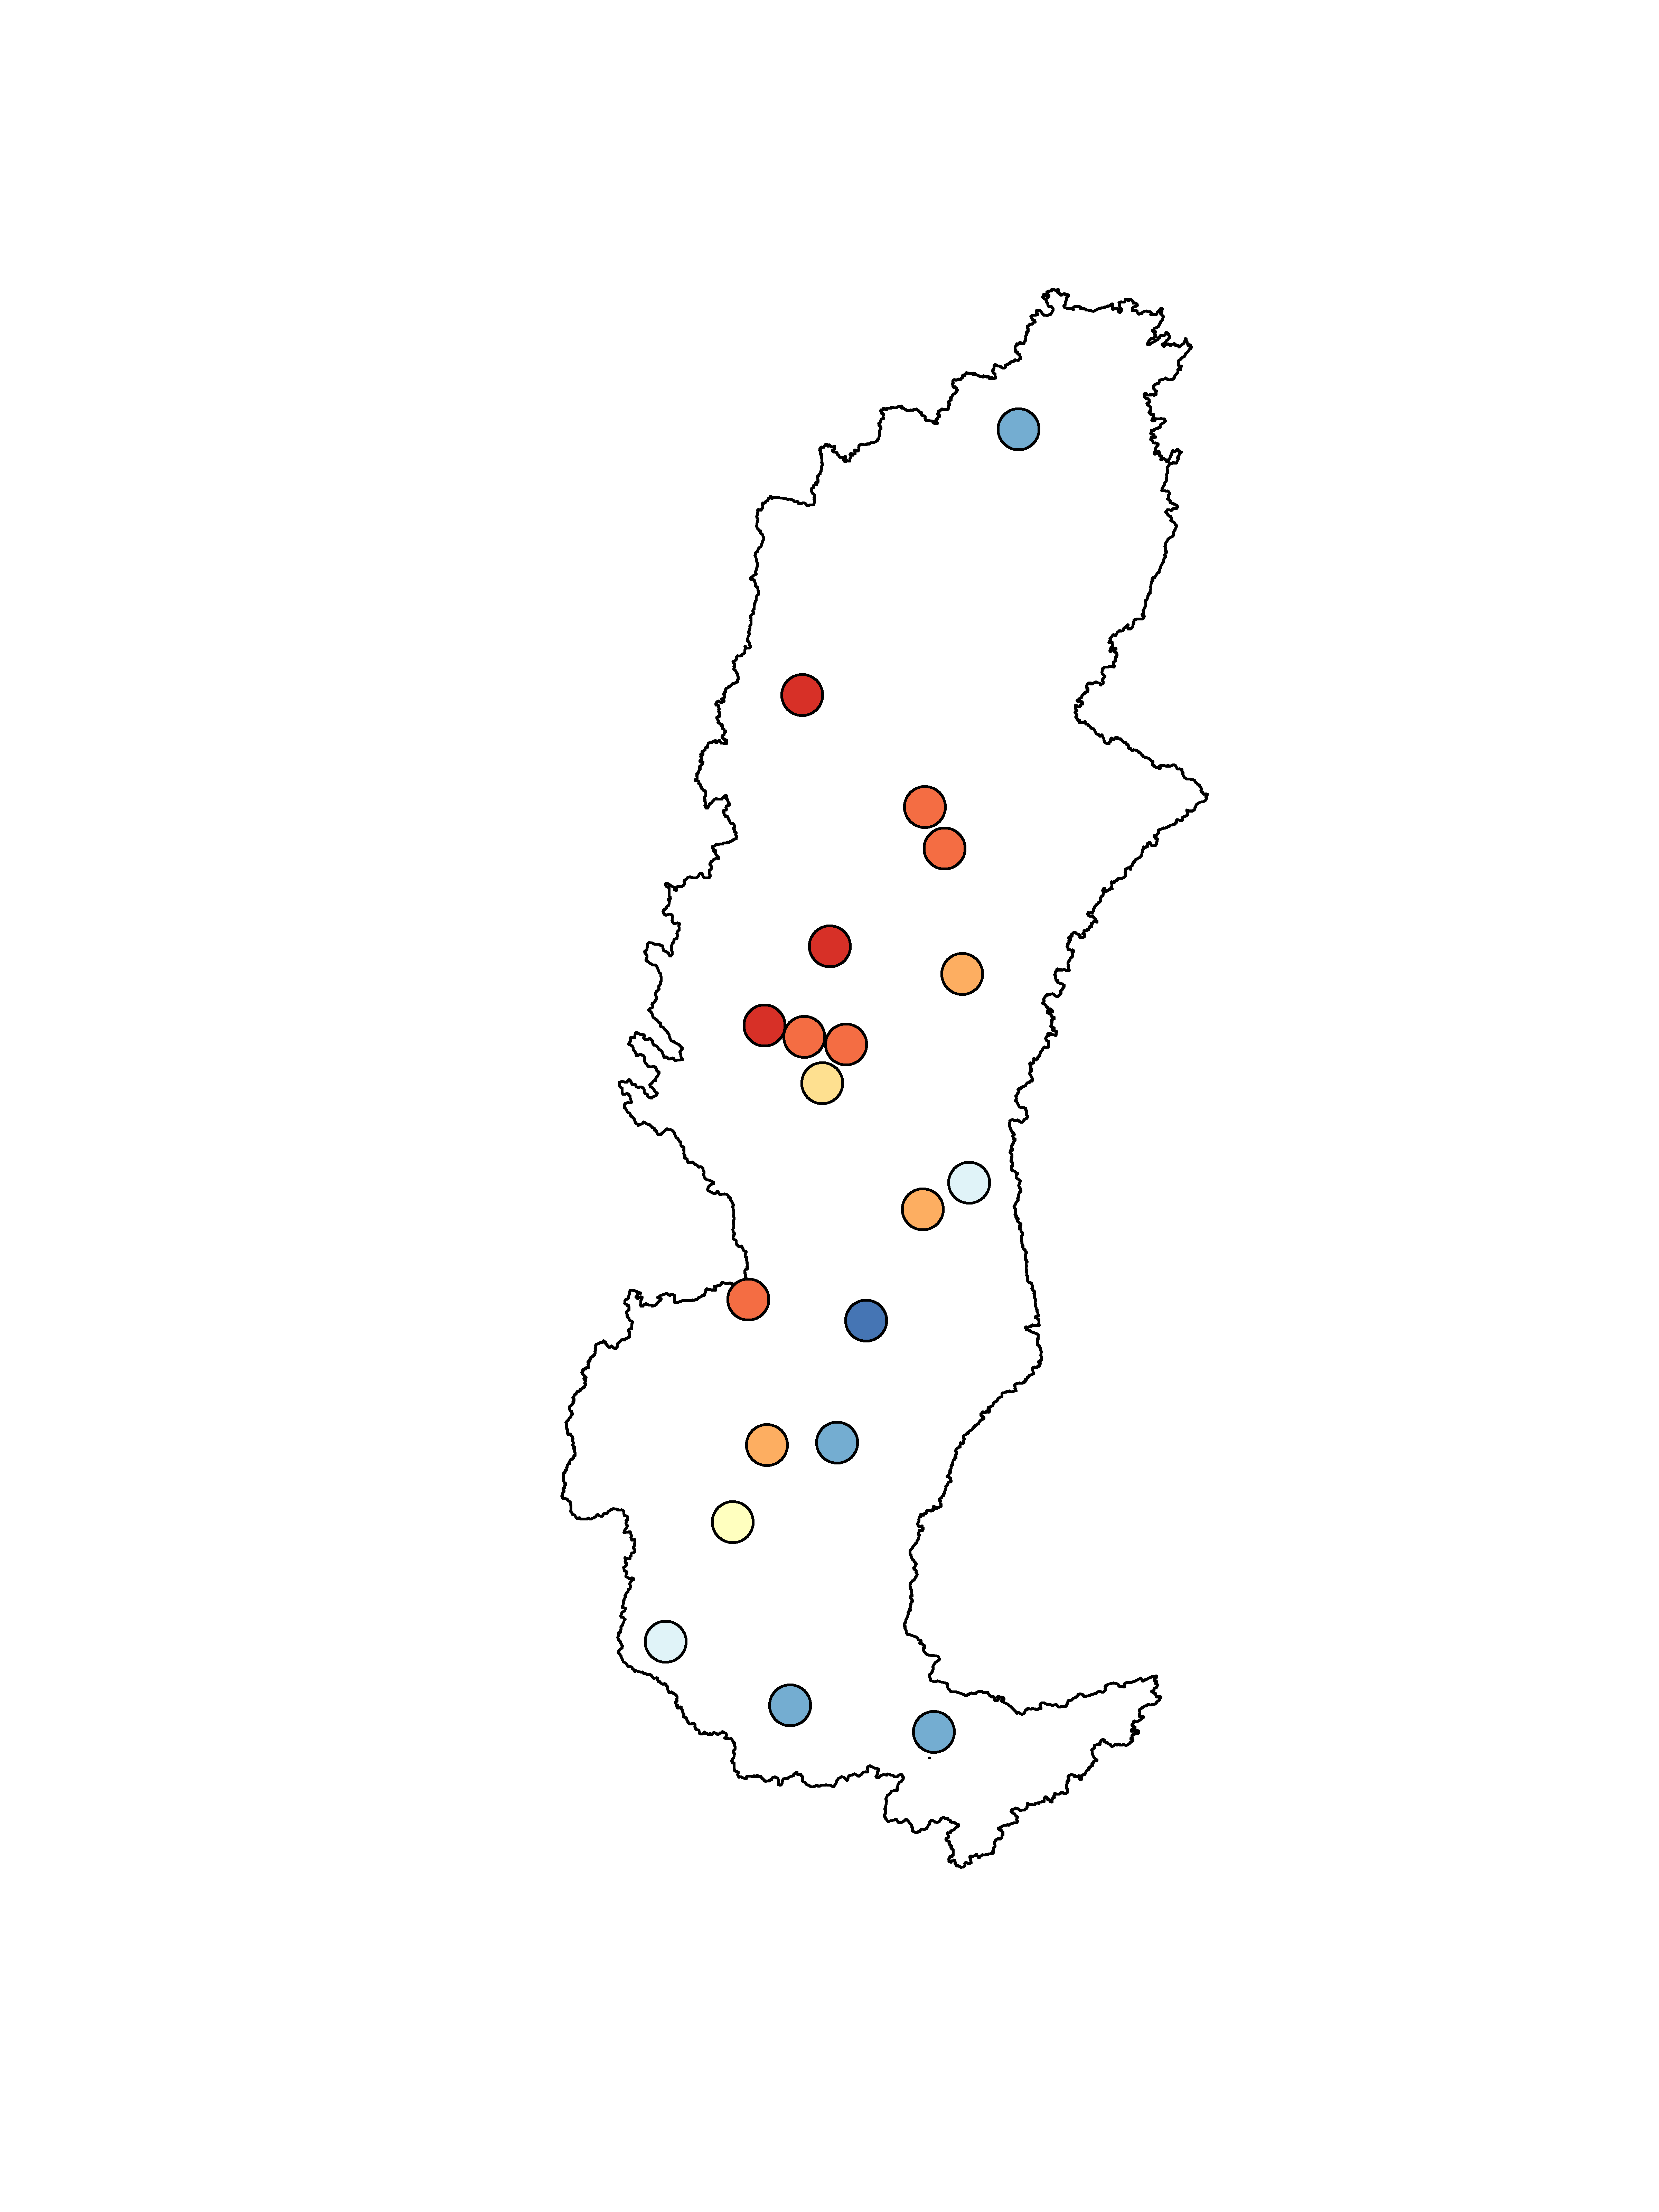
\includegraphics[trim= 4cm 2cm 1cm 2cm, clip, scale = 0.35]{./img/nashsut_penman} &
				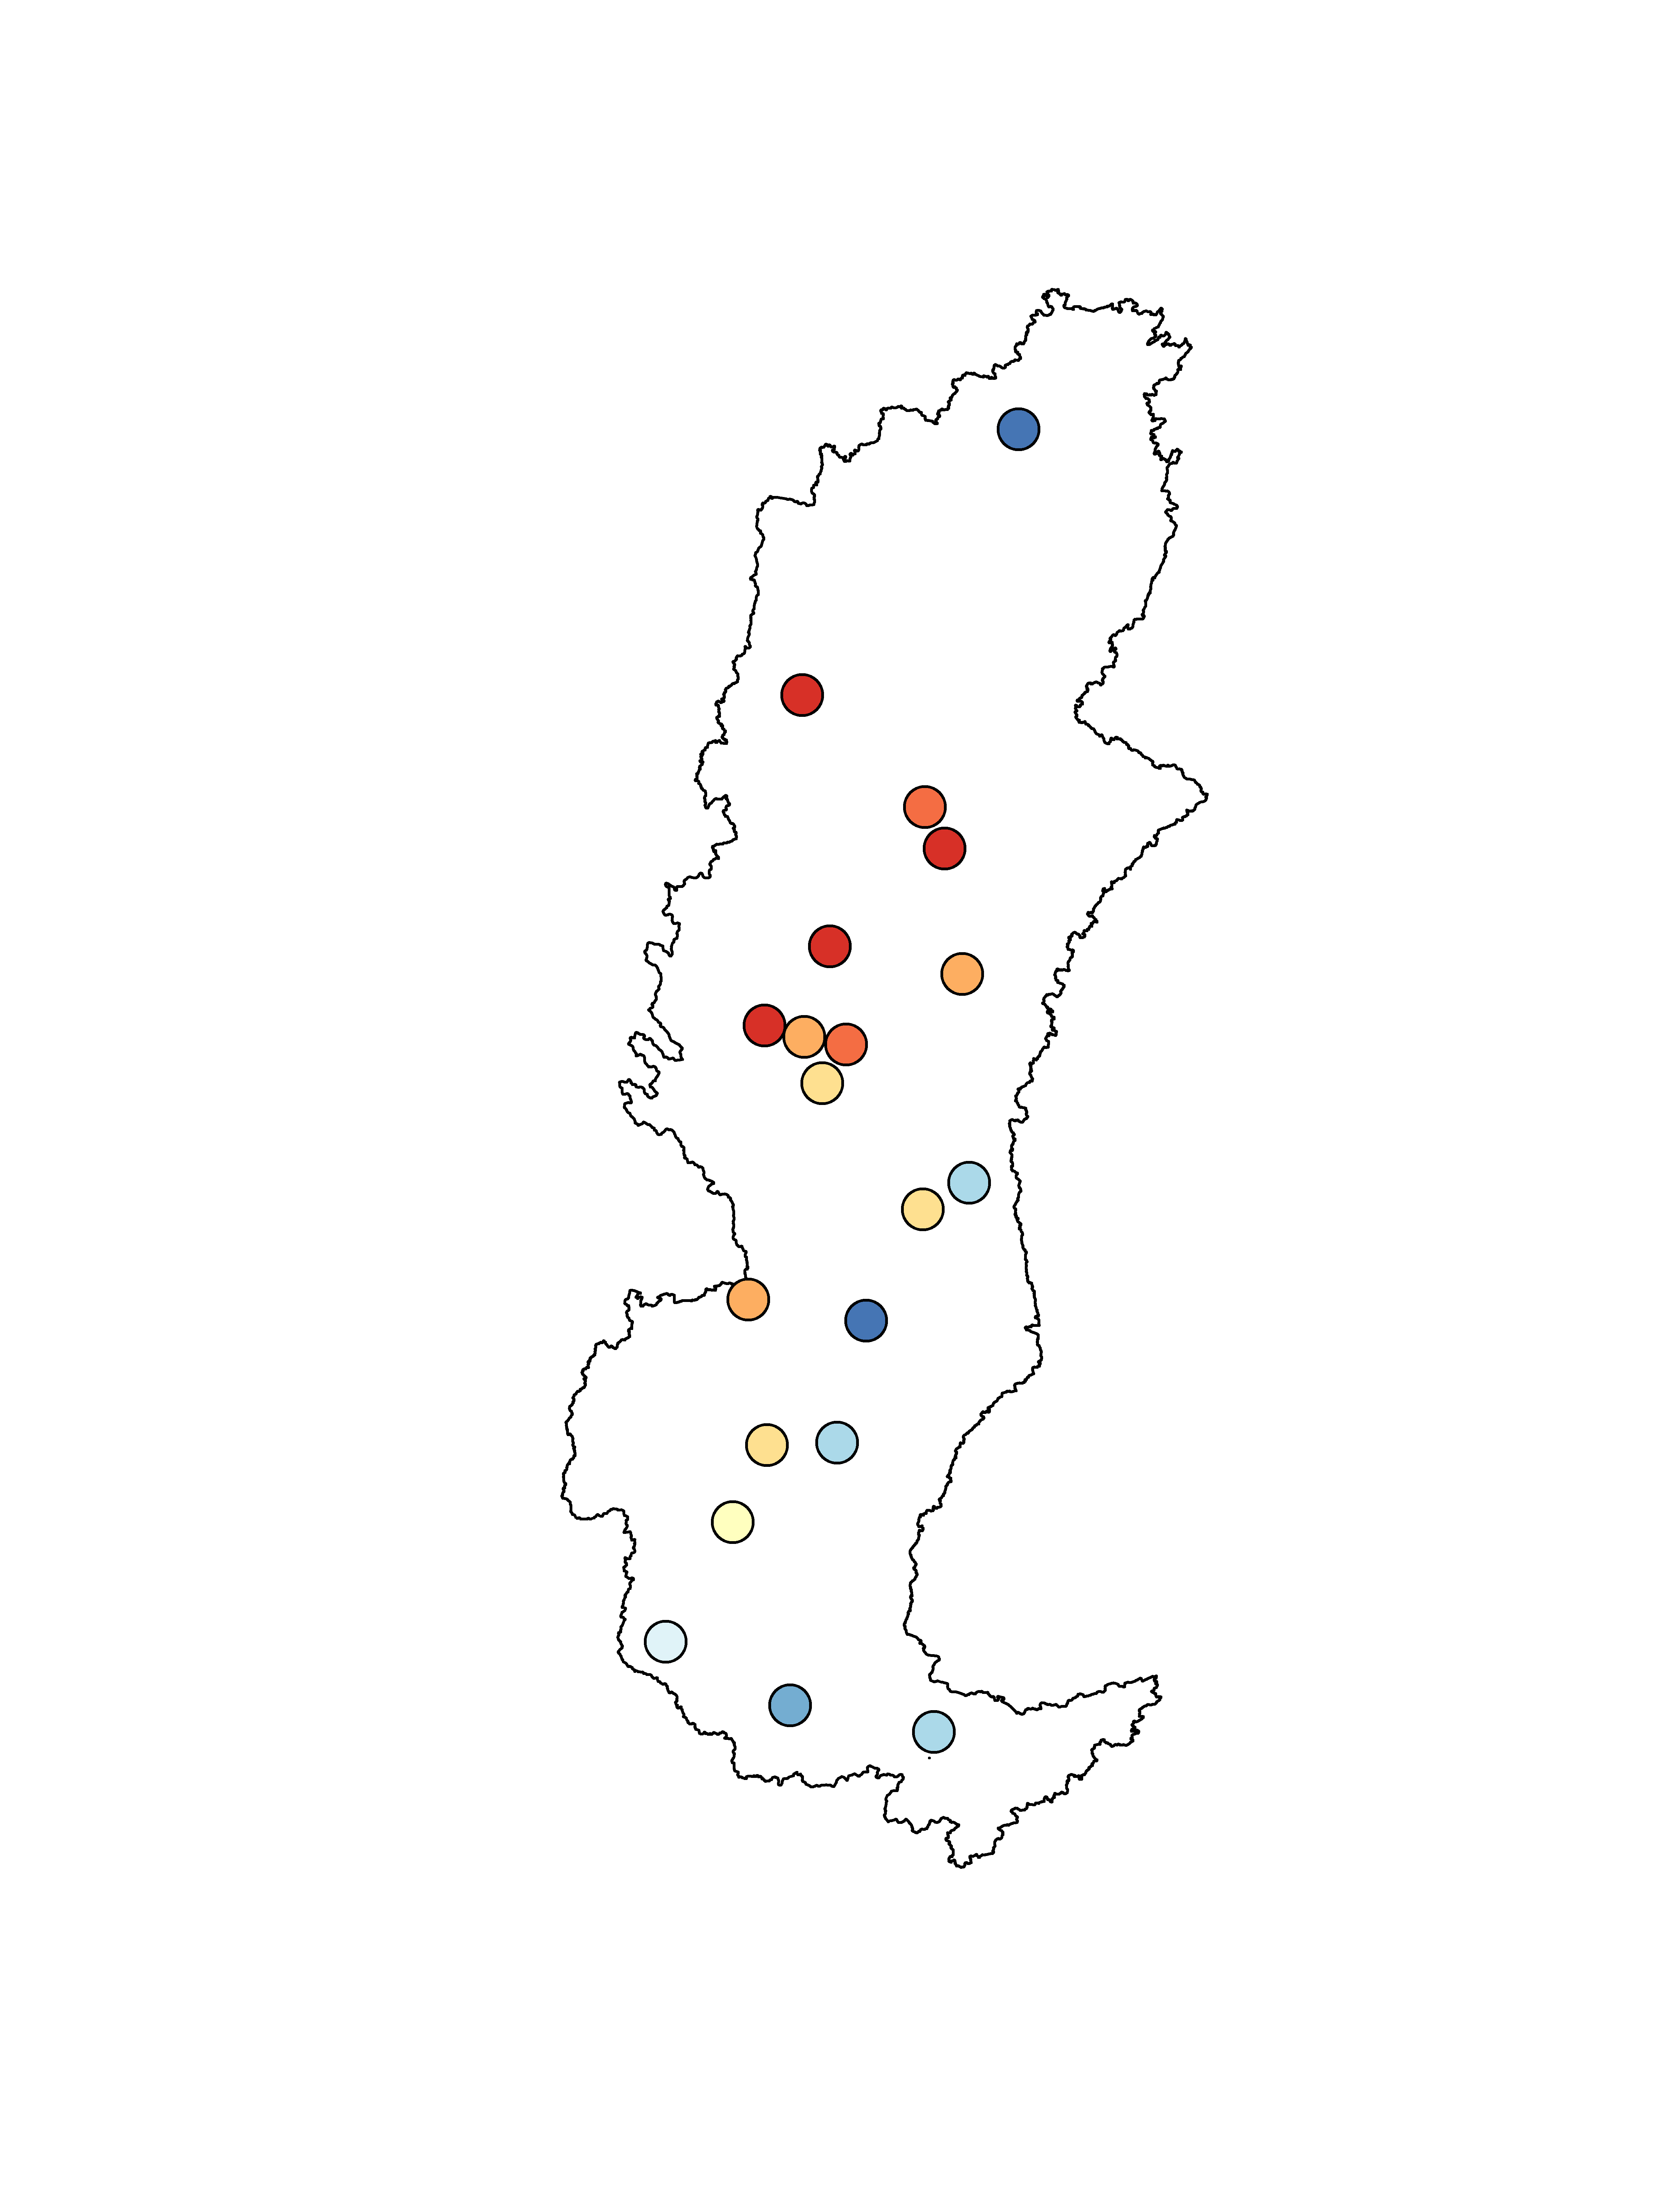
\includegraphics[trim= 4cm 2cm 1cm 2cm, clip, scale = 0.35]{./img/nashsut_priestley} &
					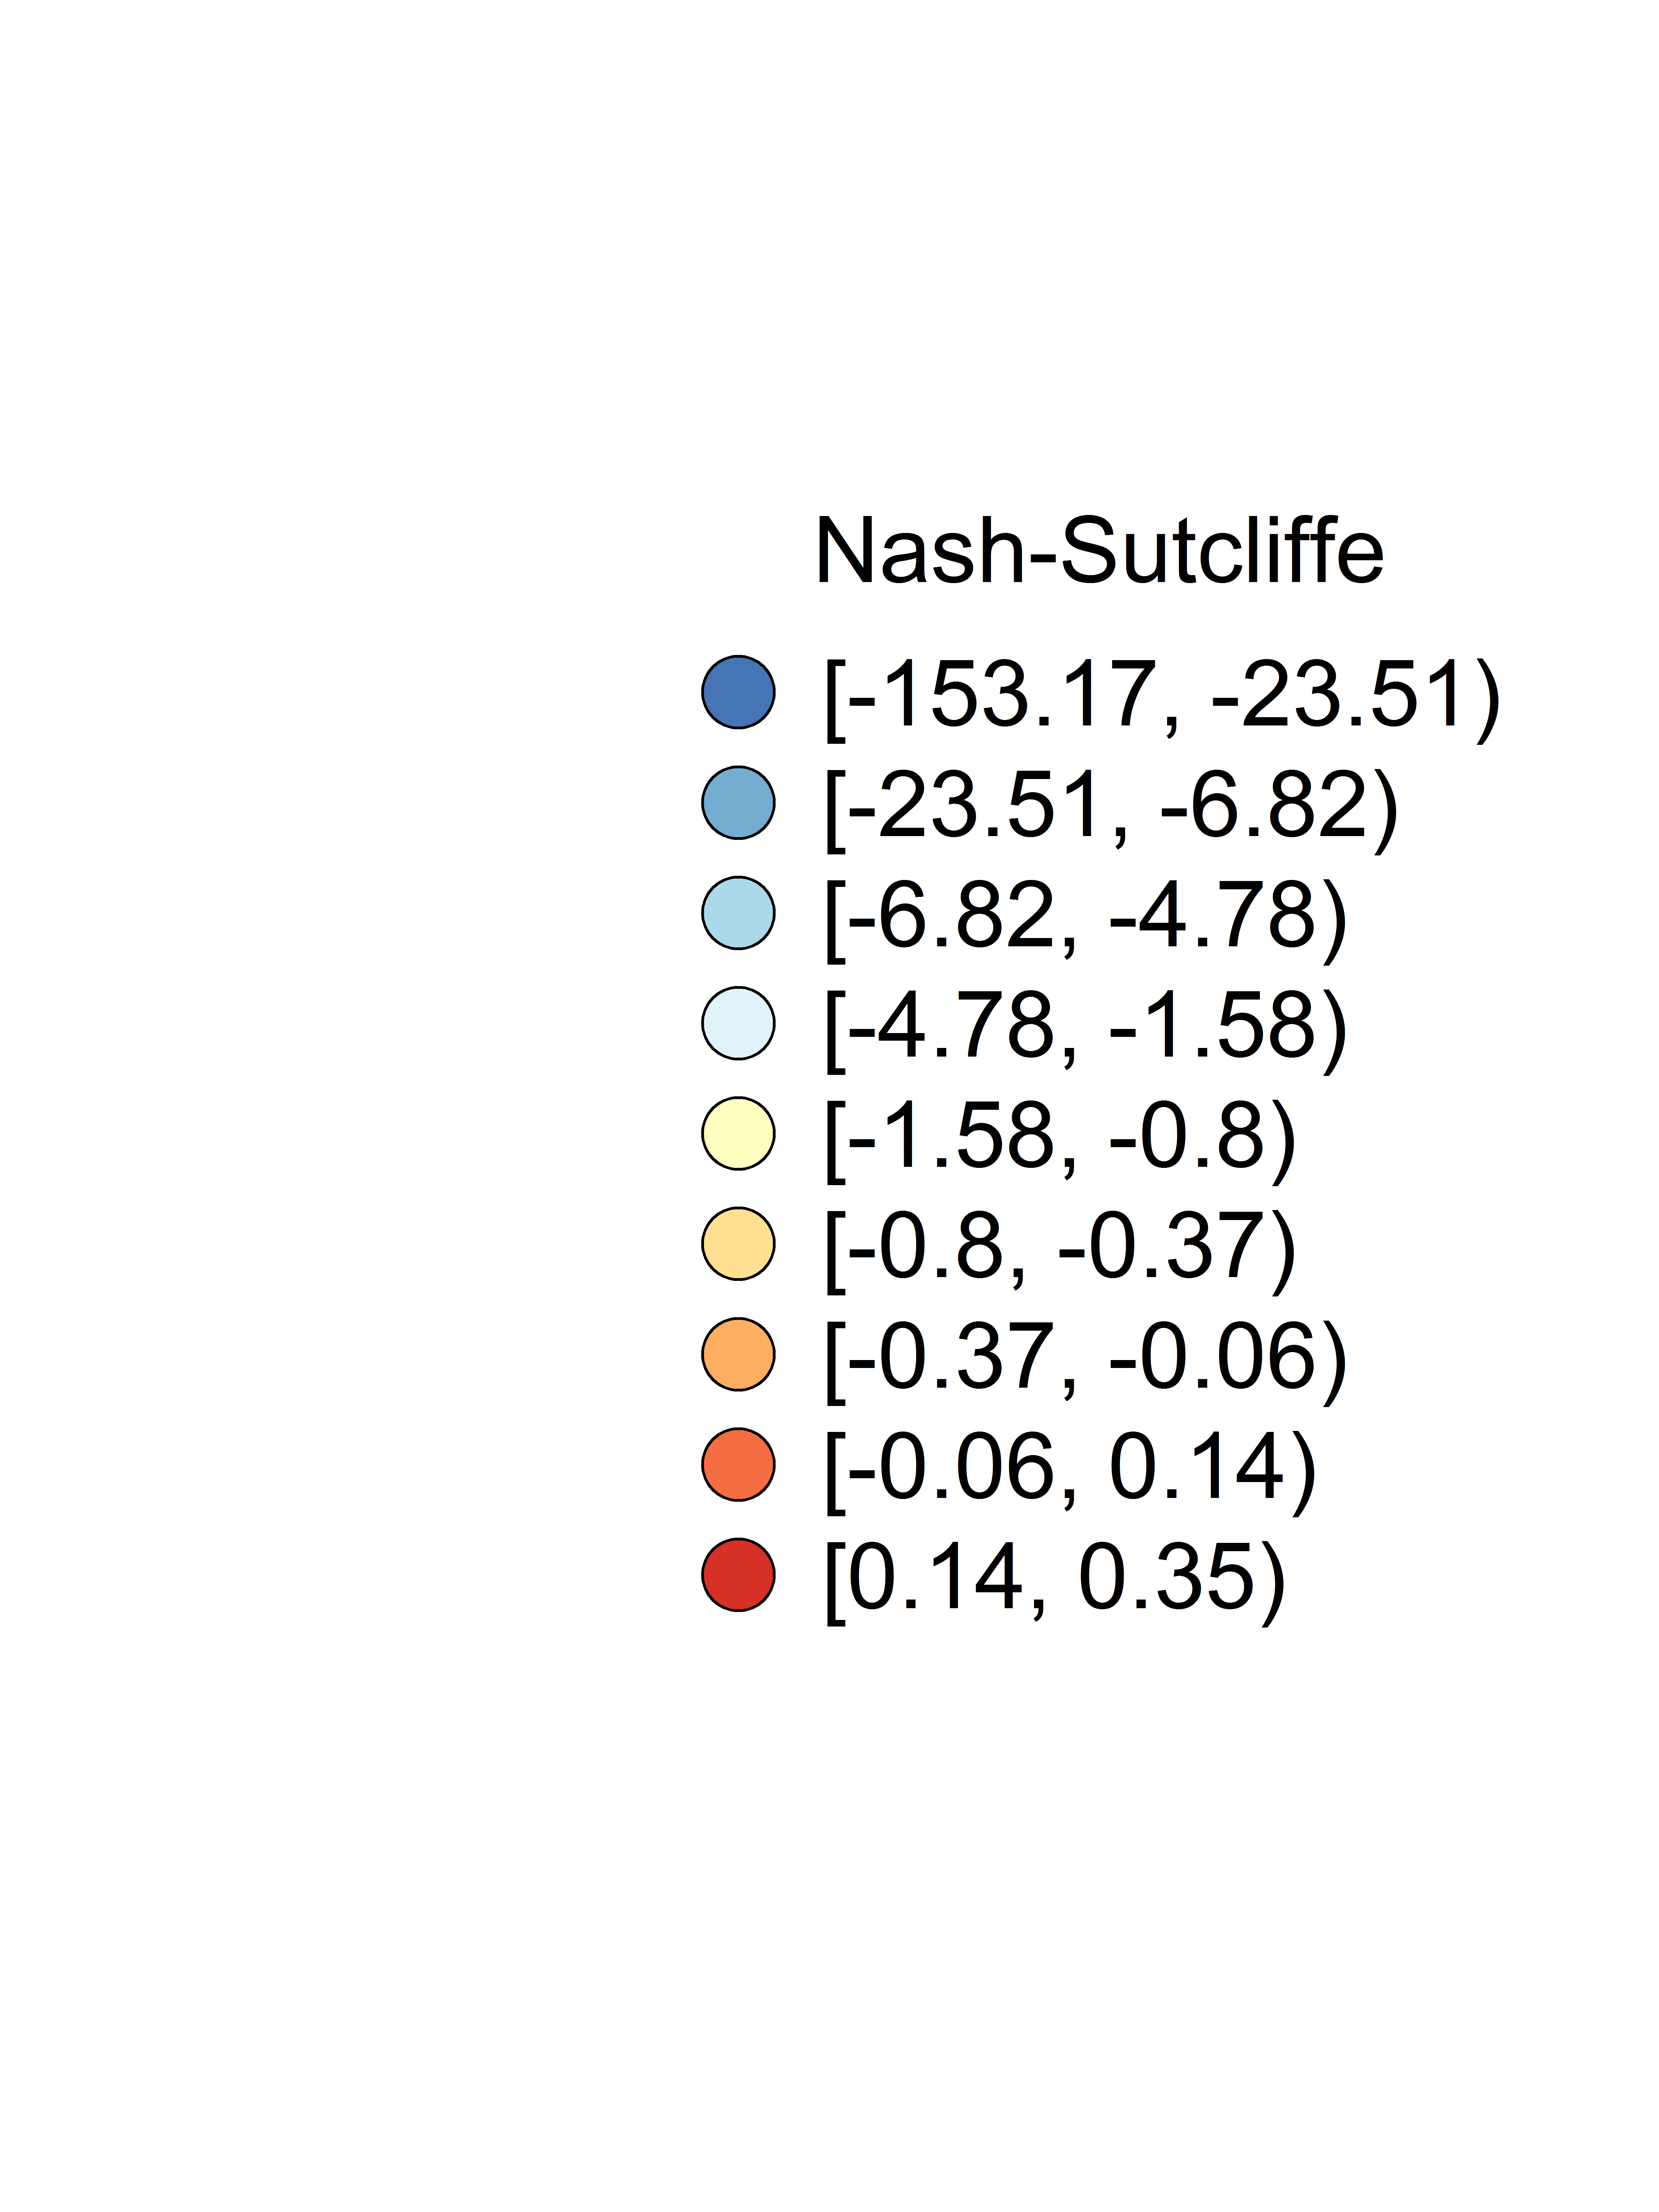
\includegraphics[trim= 5cm 2cm 0cm 3cm, clip, scale = 0.3]{./img/nashsut_legend} \\			
	\end{tabular}
	\caption[Three evapotranspiration methods were examined, Hargreaves]{Three evapotranspiration methods were examined, Hargreaves, Penman--Monteith, and Priestley--Taylor (displayed left to right) each of which was assessed for how well the simulated streamflow matched observed streamflow sites, the value of each is displayed in each map. Each method was assessed using percent bias (top three maps) and the Nash-Sutcliffe model efficiency coefficient (bottom three maps). The Penman--Monteith equation provided the best fit to observed streamflow.}
	\label{fig:et_methods}
\end{figure}
\end{landscape}

%%Observed vs pred Ponds
\begin{figure}[H]
	\centering
	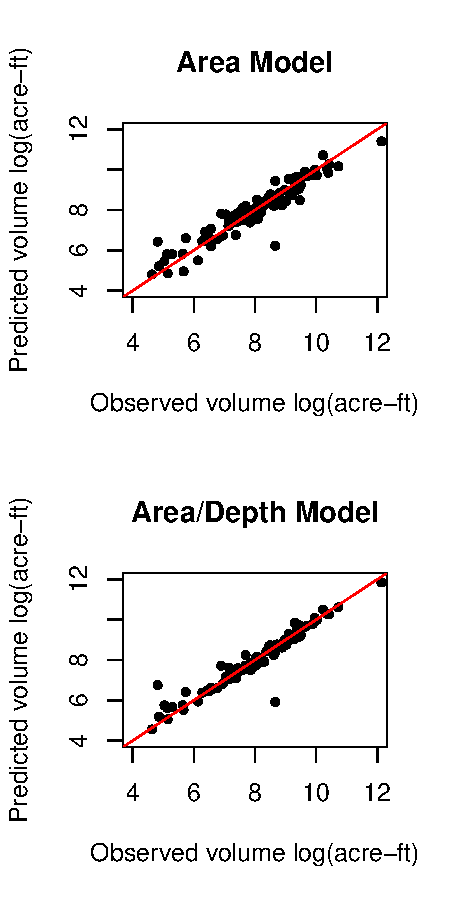
\includegraphics[width=0.6\textwidth]{./img/area_model_observed_predicted.pdf}
	\caption[Scatterplots of observed versus predicted lake volumes]{Scatterplots of observed versus predicted lake volumes used to parameterize geometric properties of ponds in SWAT. The area/depth model used lake surface area and maximum depth to predict lake volume and the area model used only lake surface area to predict its volume. The area/depth model explains 92\% of the variability in volumes and the area model explains 89\% of the variability in volumes.}
	\label{fig:volume_regressions}
\end{figure}

%%%%   Filled DEM
\begin{figure}[H]
	\centering
	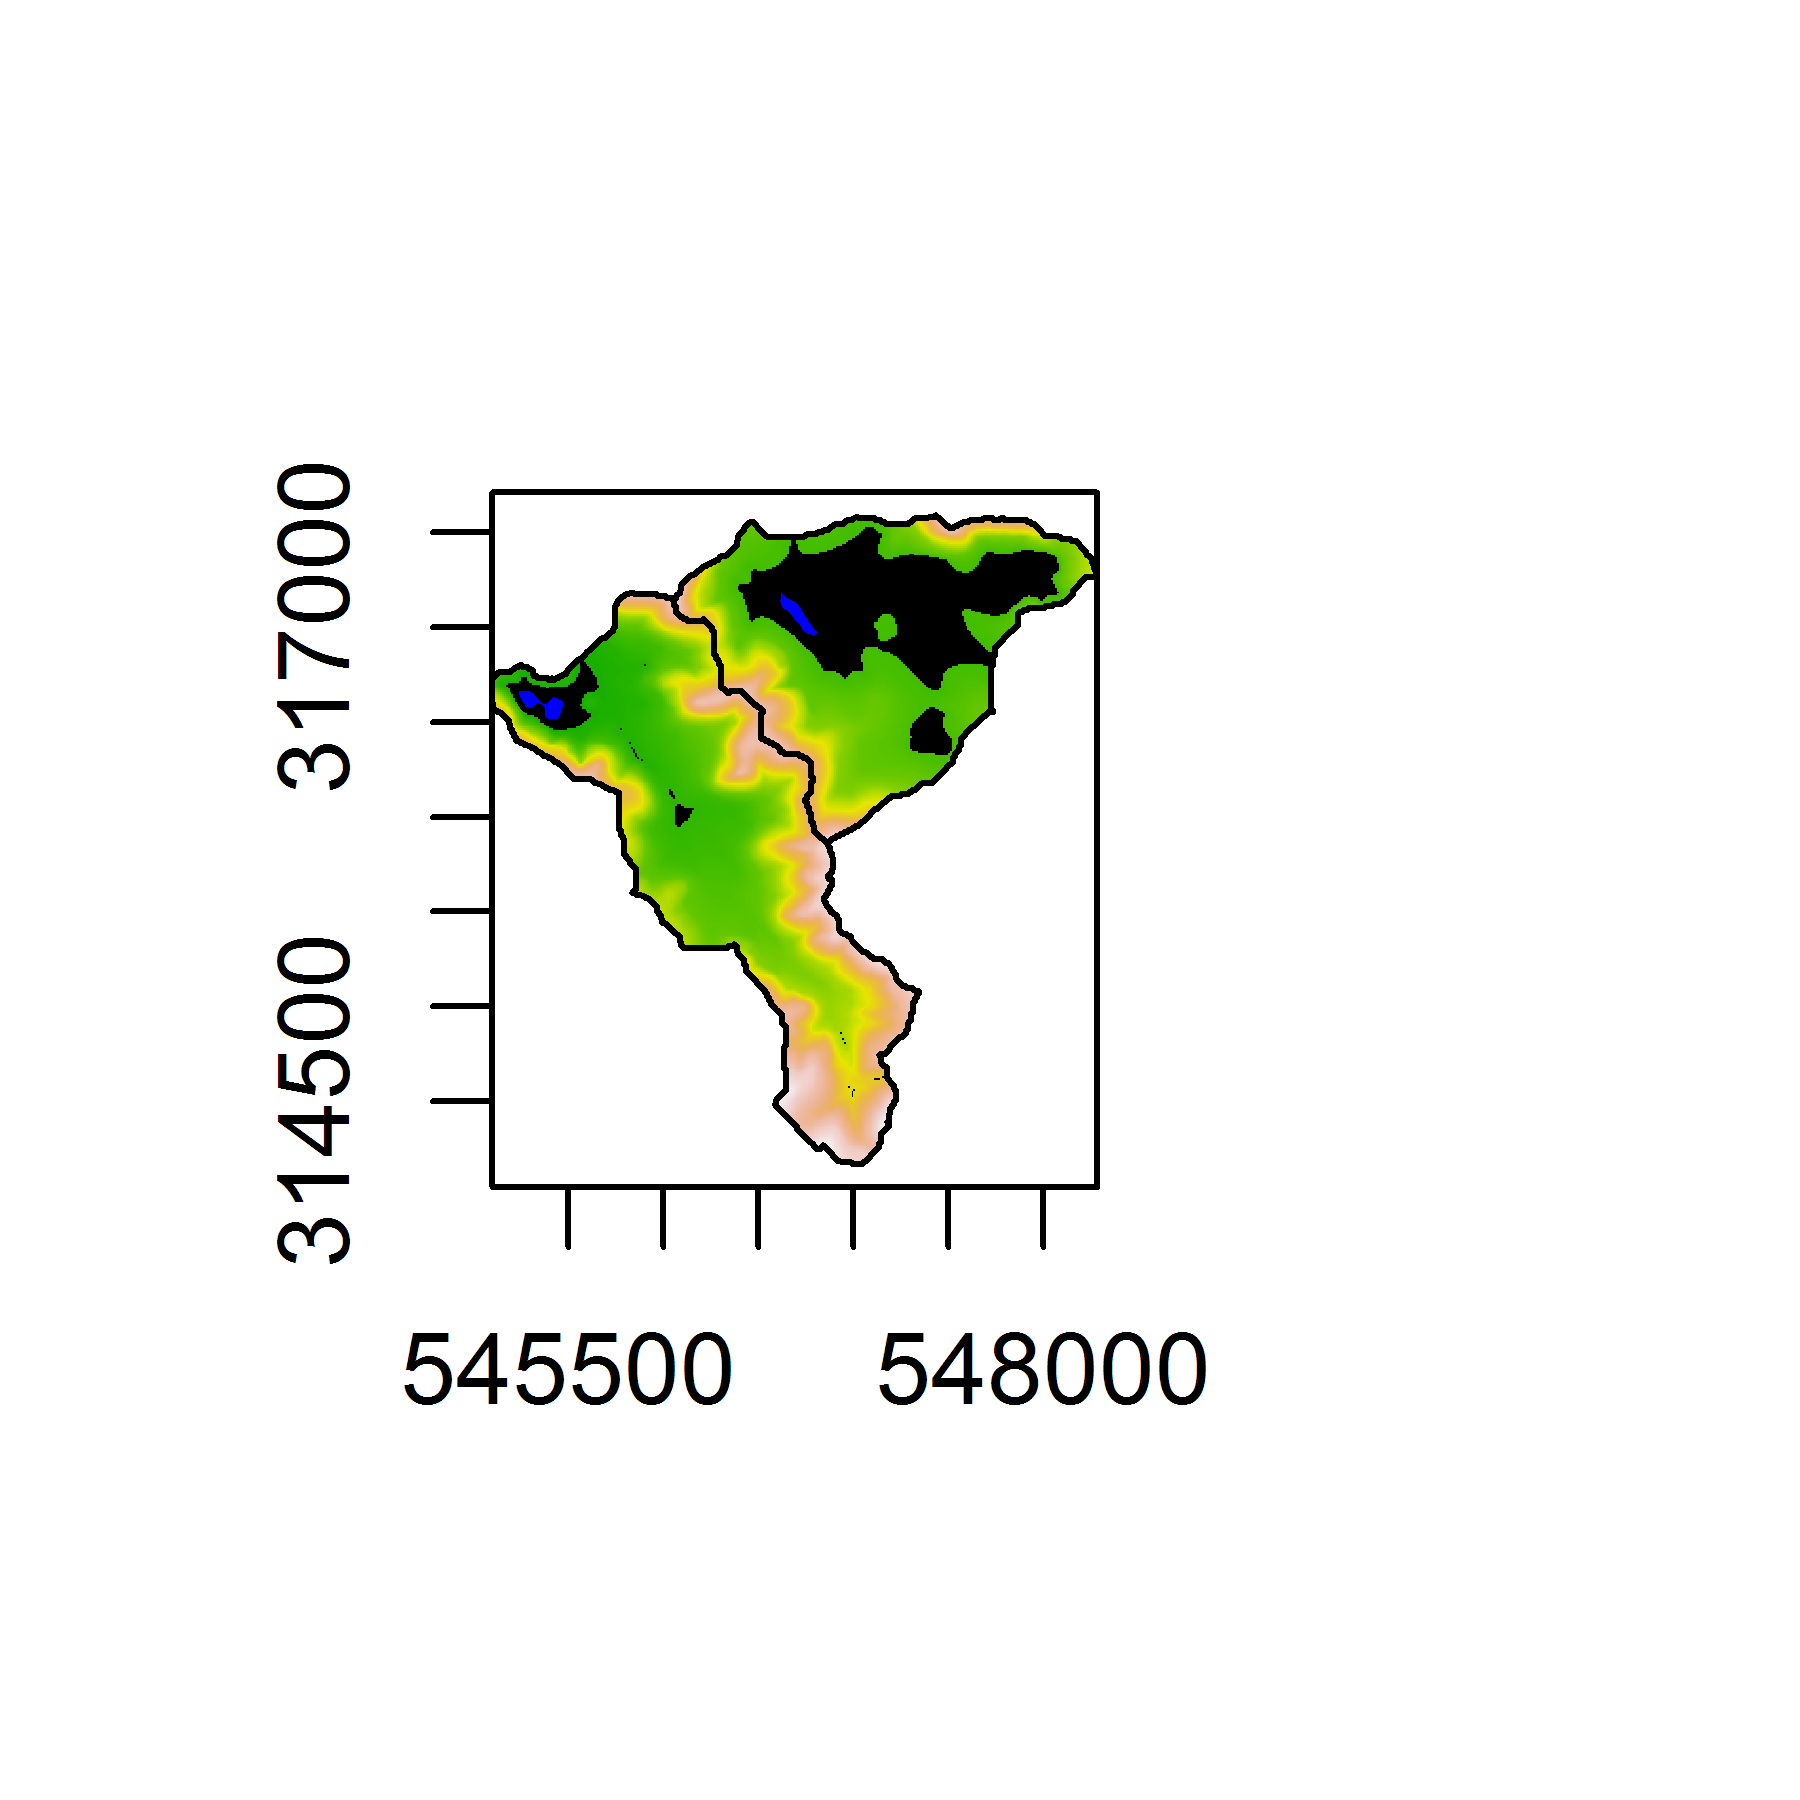
\includegraphics[width=0.6\textwidth]{./img/maximum_pond_volume.png}
	\caption{Example image of a filled digital elevation model (DEM) used to estimate maximum storage volume and surface area of landlocked lakes for parameterizing geometries of ponds in SWAT. The green to white gradient represents elevation from low to high. Blue polygons are landlocked lakes. Black polygons are the extent of grid cells associated with the internally draining area that flows to a landlocked lake. Black polygons not intersecting a landlocked lake were not used in surface area and volume calculations. The x and y axes are for scale---they are in units of meters from the origin of the Wisconsin Transverse Mercator projection.}
	\label{fig:maximum_pond_volume}
\end{figure}

%%Ponds & wetlands
\begin{figure}[h!]
	\centering
	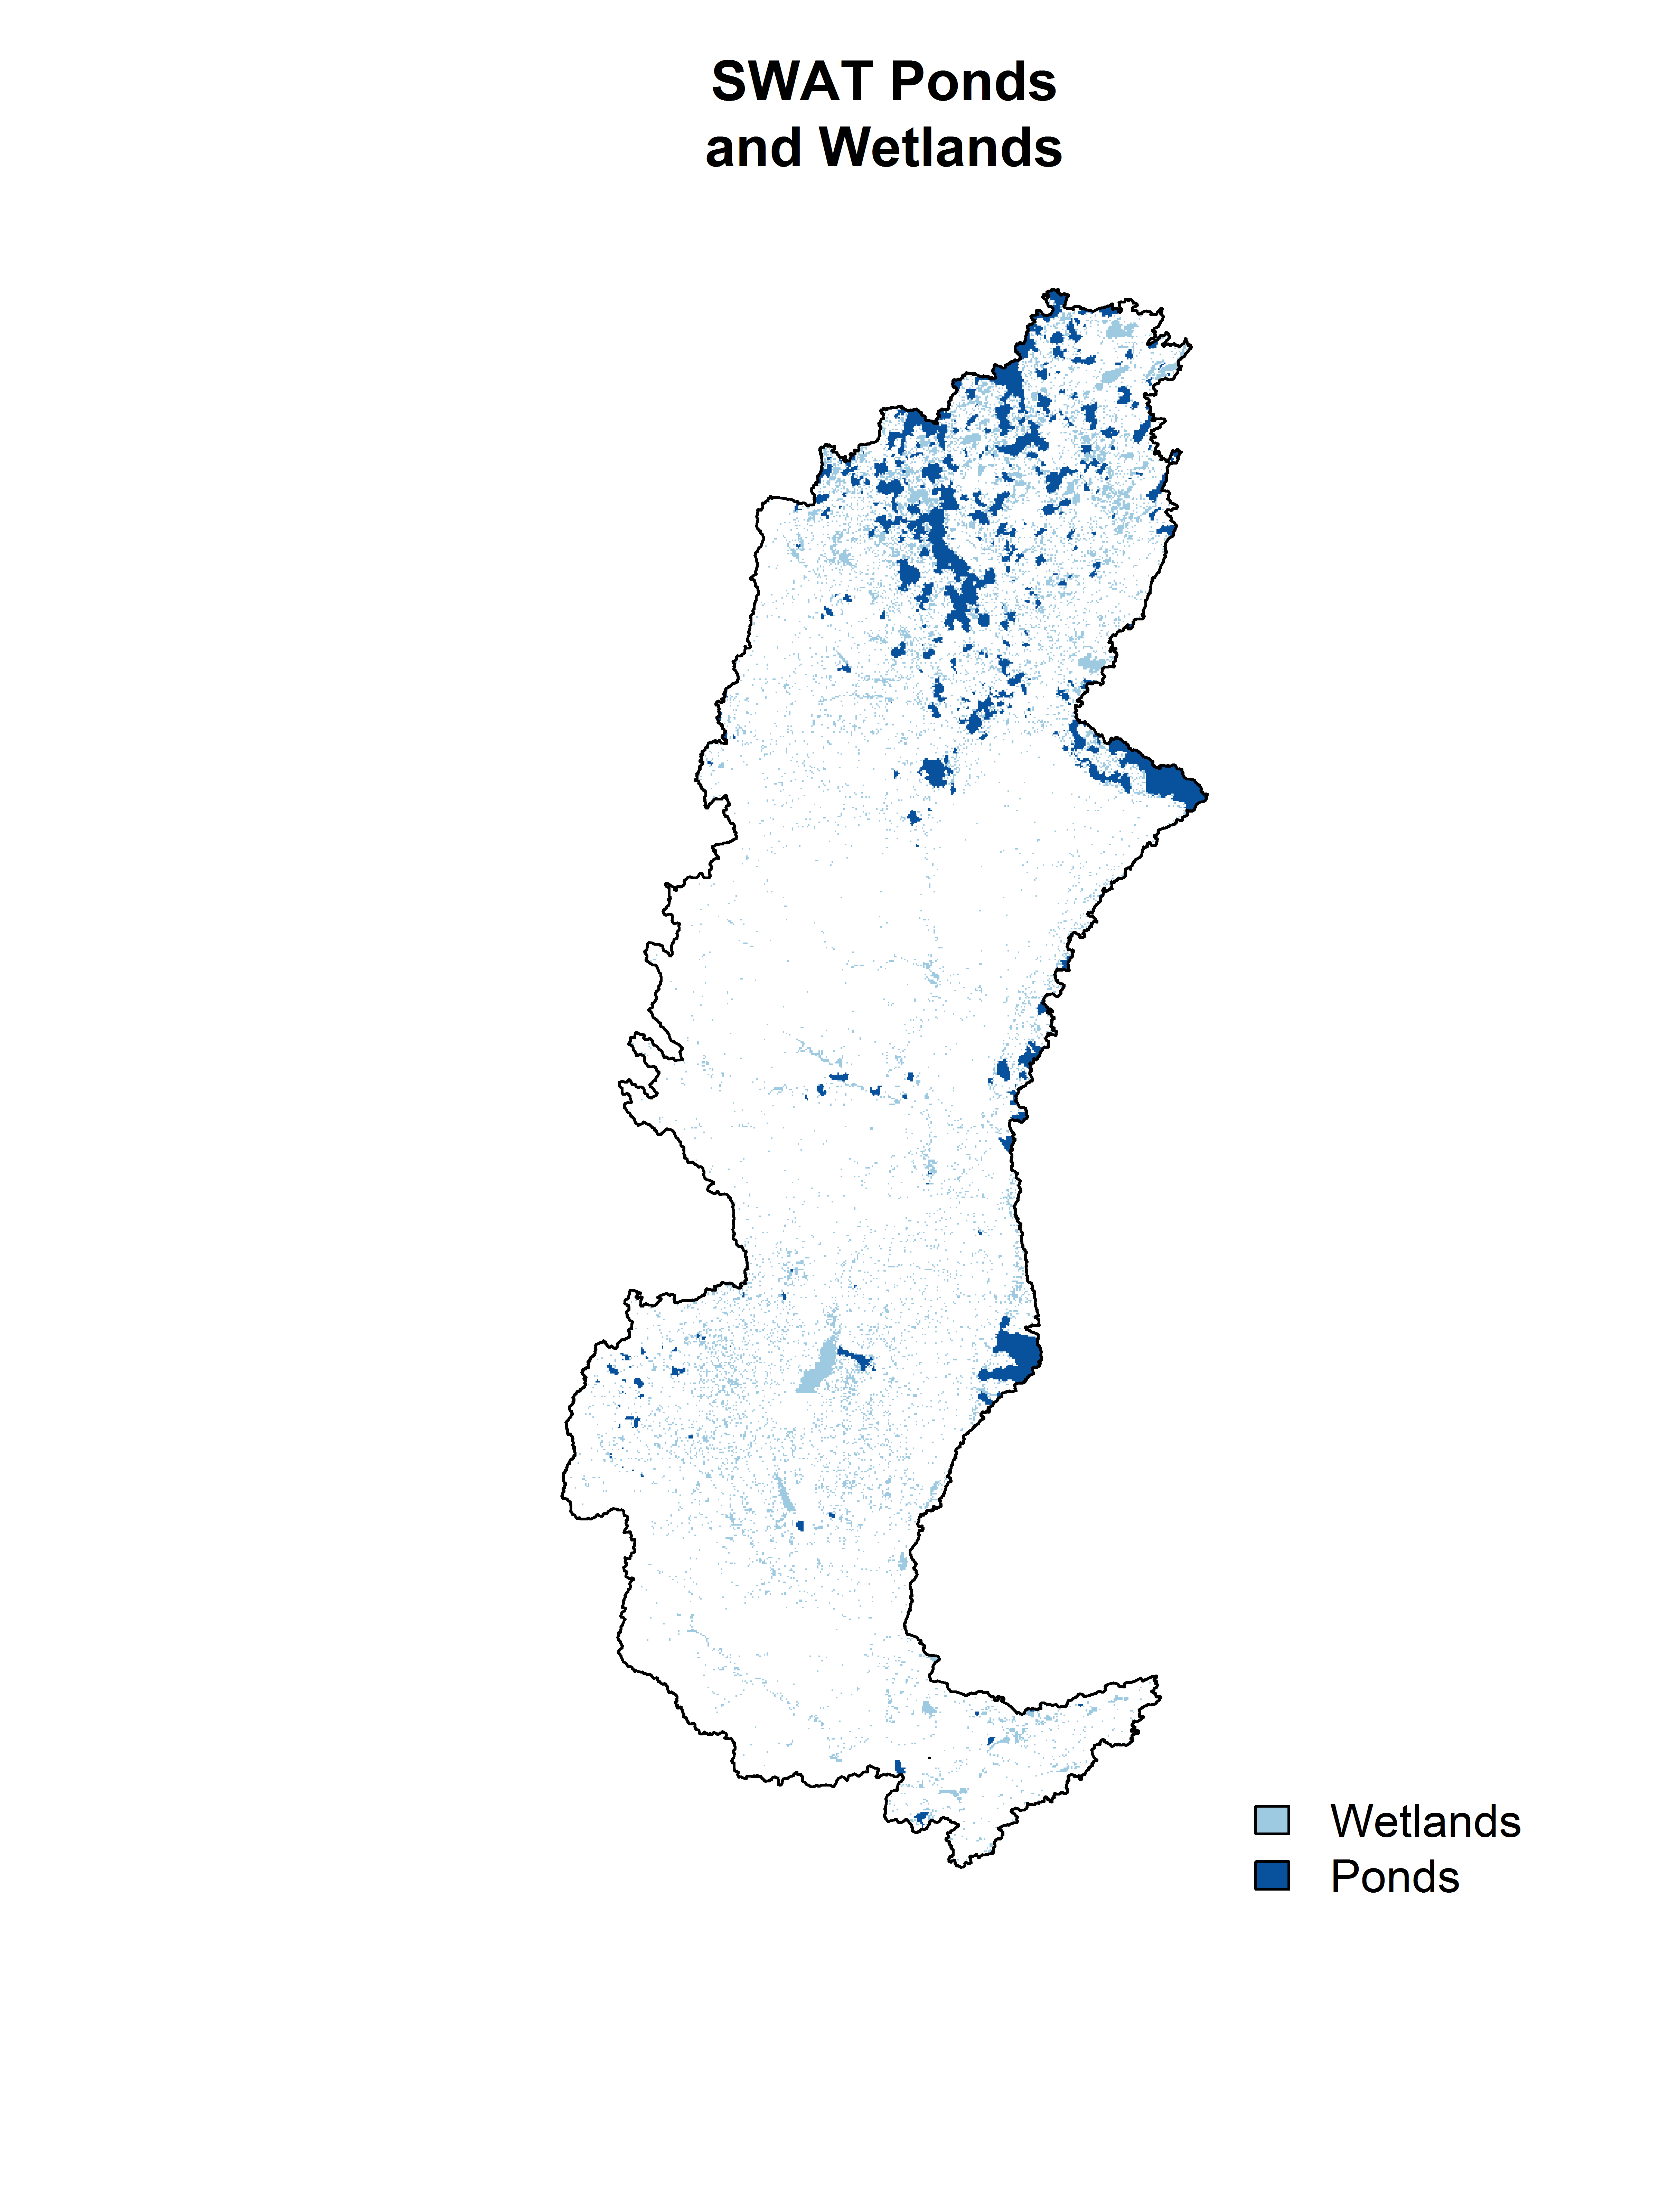
\includegraphics[width=\textwidth]{./img/wetlands_and_ponds.png}
	\caption{Map showing the location of the SWAT ponds and wetlands in the Wisconsin River Basin.}
	\label{fig:wetlands_and_ponds}
\end{figure}

%%ALPHA_BF scatterplot
\begin{figure}
	\centering
	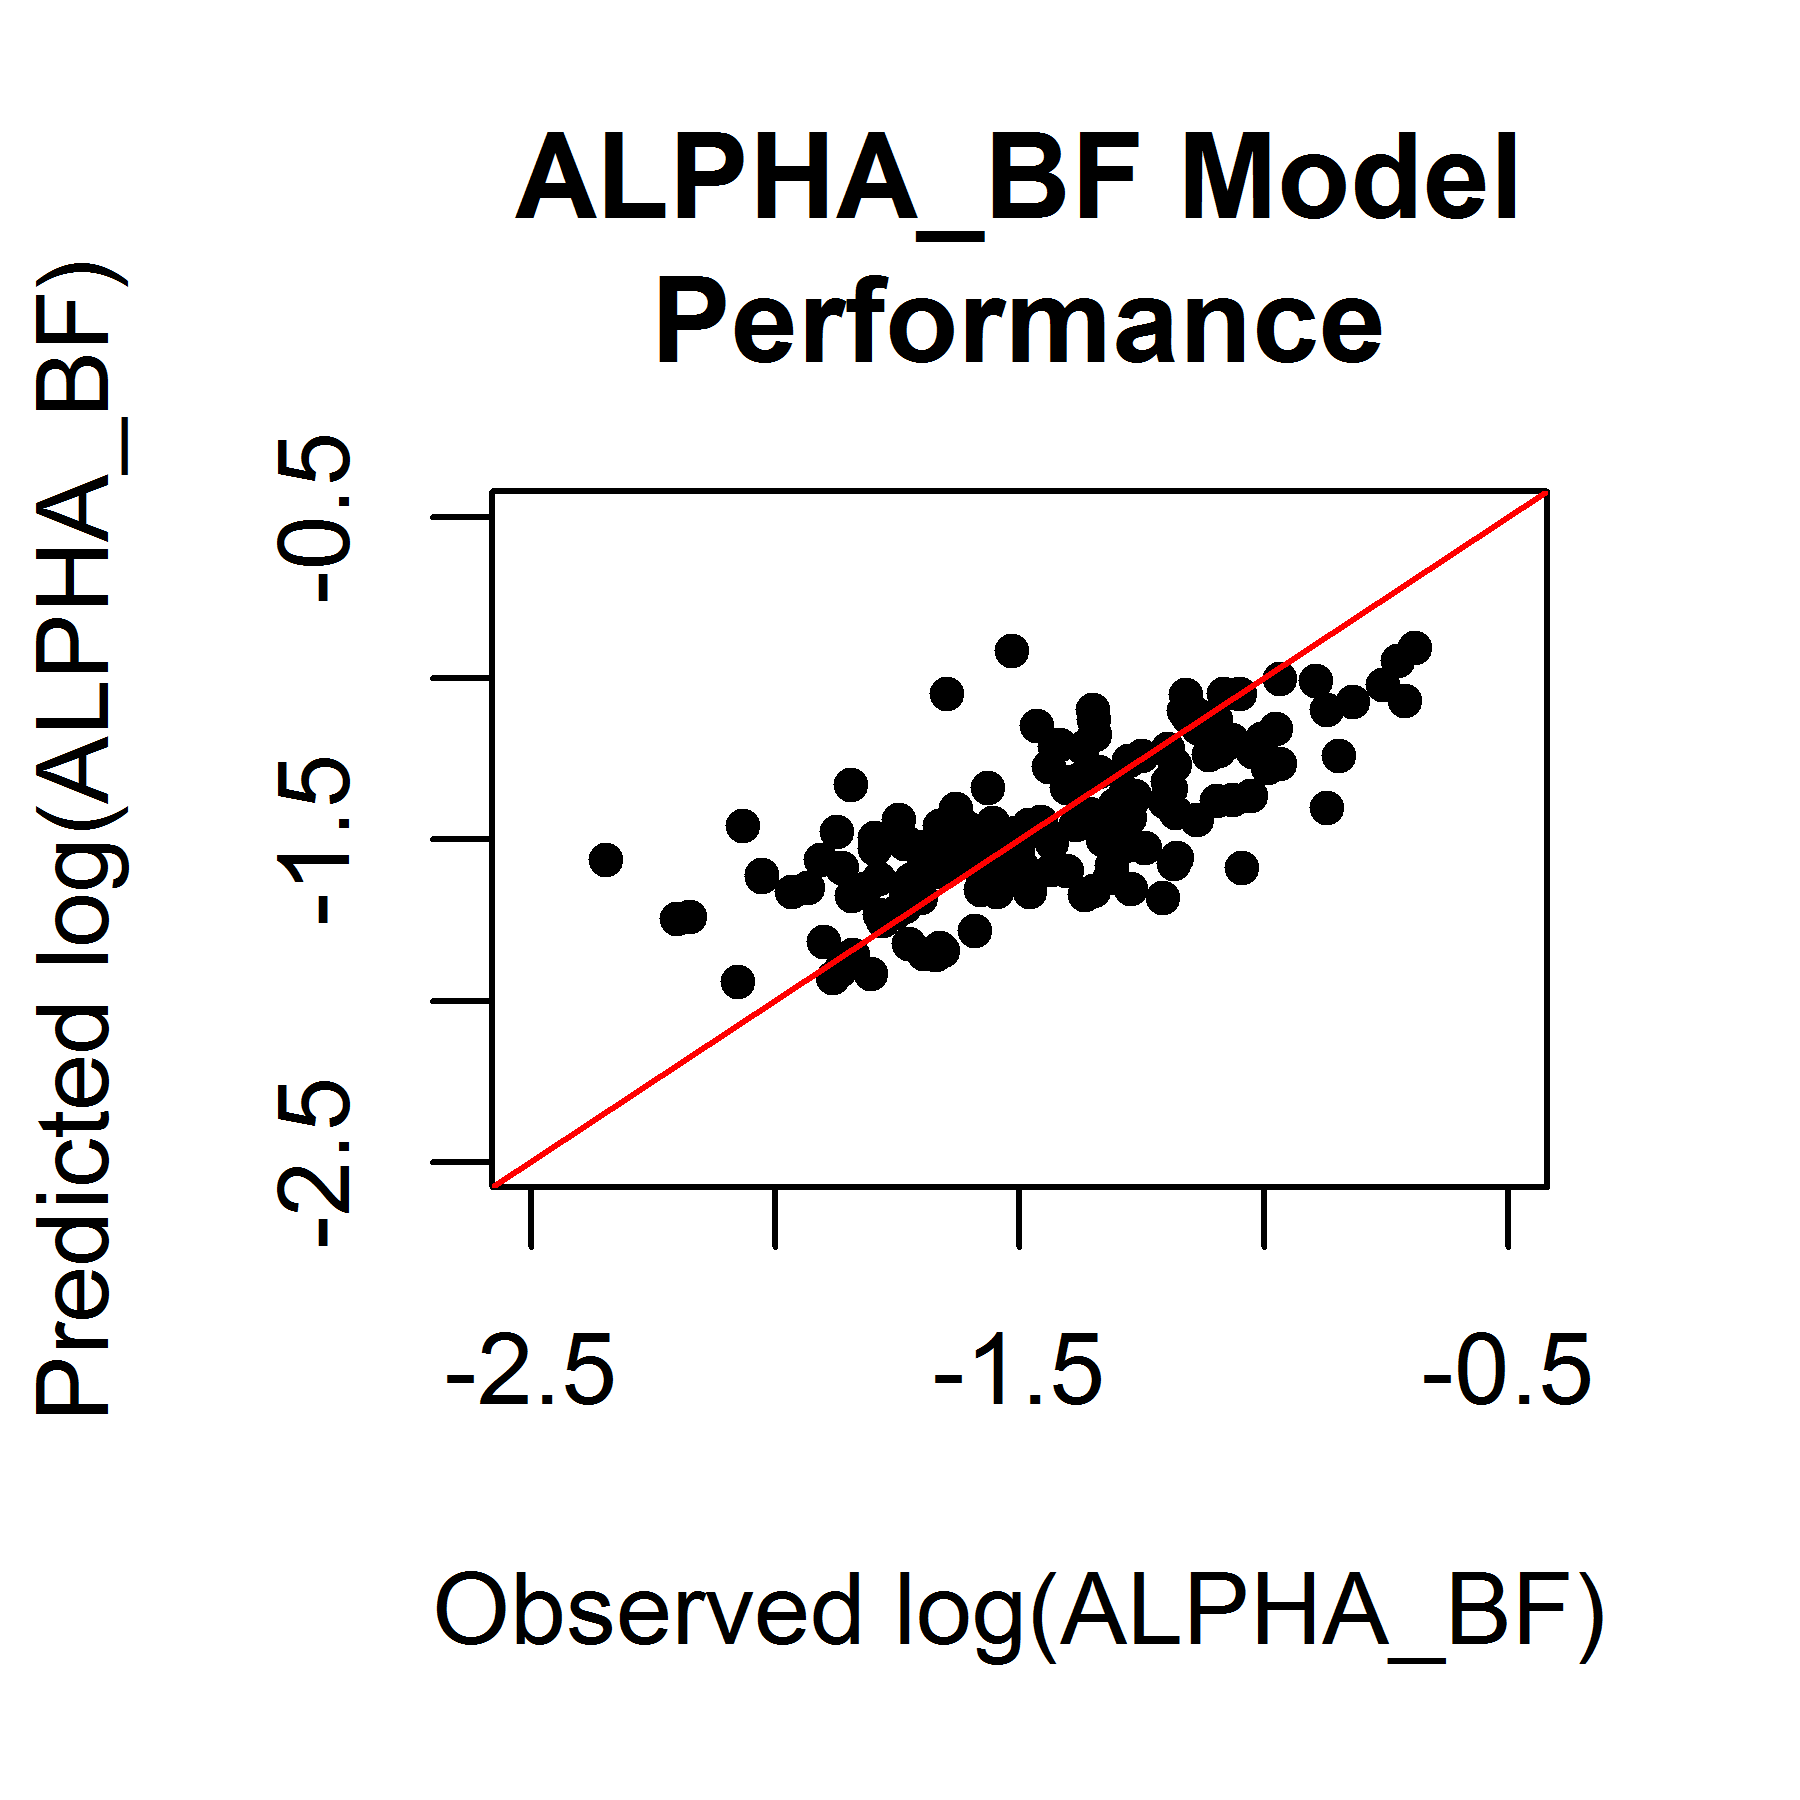
\includegraphics[width=0.5\textwidth]{./img/alpha_bf_scatterplot.png}
	\caption{Observed versus predicted ALPHA\_BF SWAT parameter. Observed ALPHA\_BF was calculated for each USGS gage site \citepalias{usgs_nwis_2014} by the Baseflow Program \citep{arnold_automated_1995}.}
	\label{fig:alpha_bf_scatterplot}
\end{figure}

\begin{figure}[h!]
	\centering
	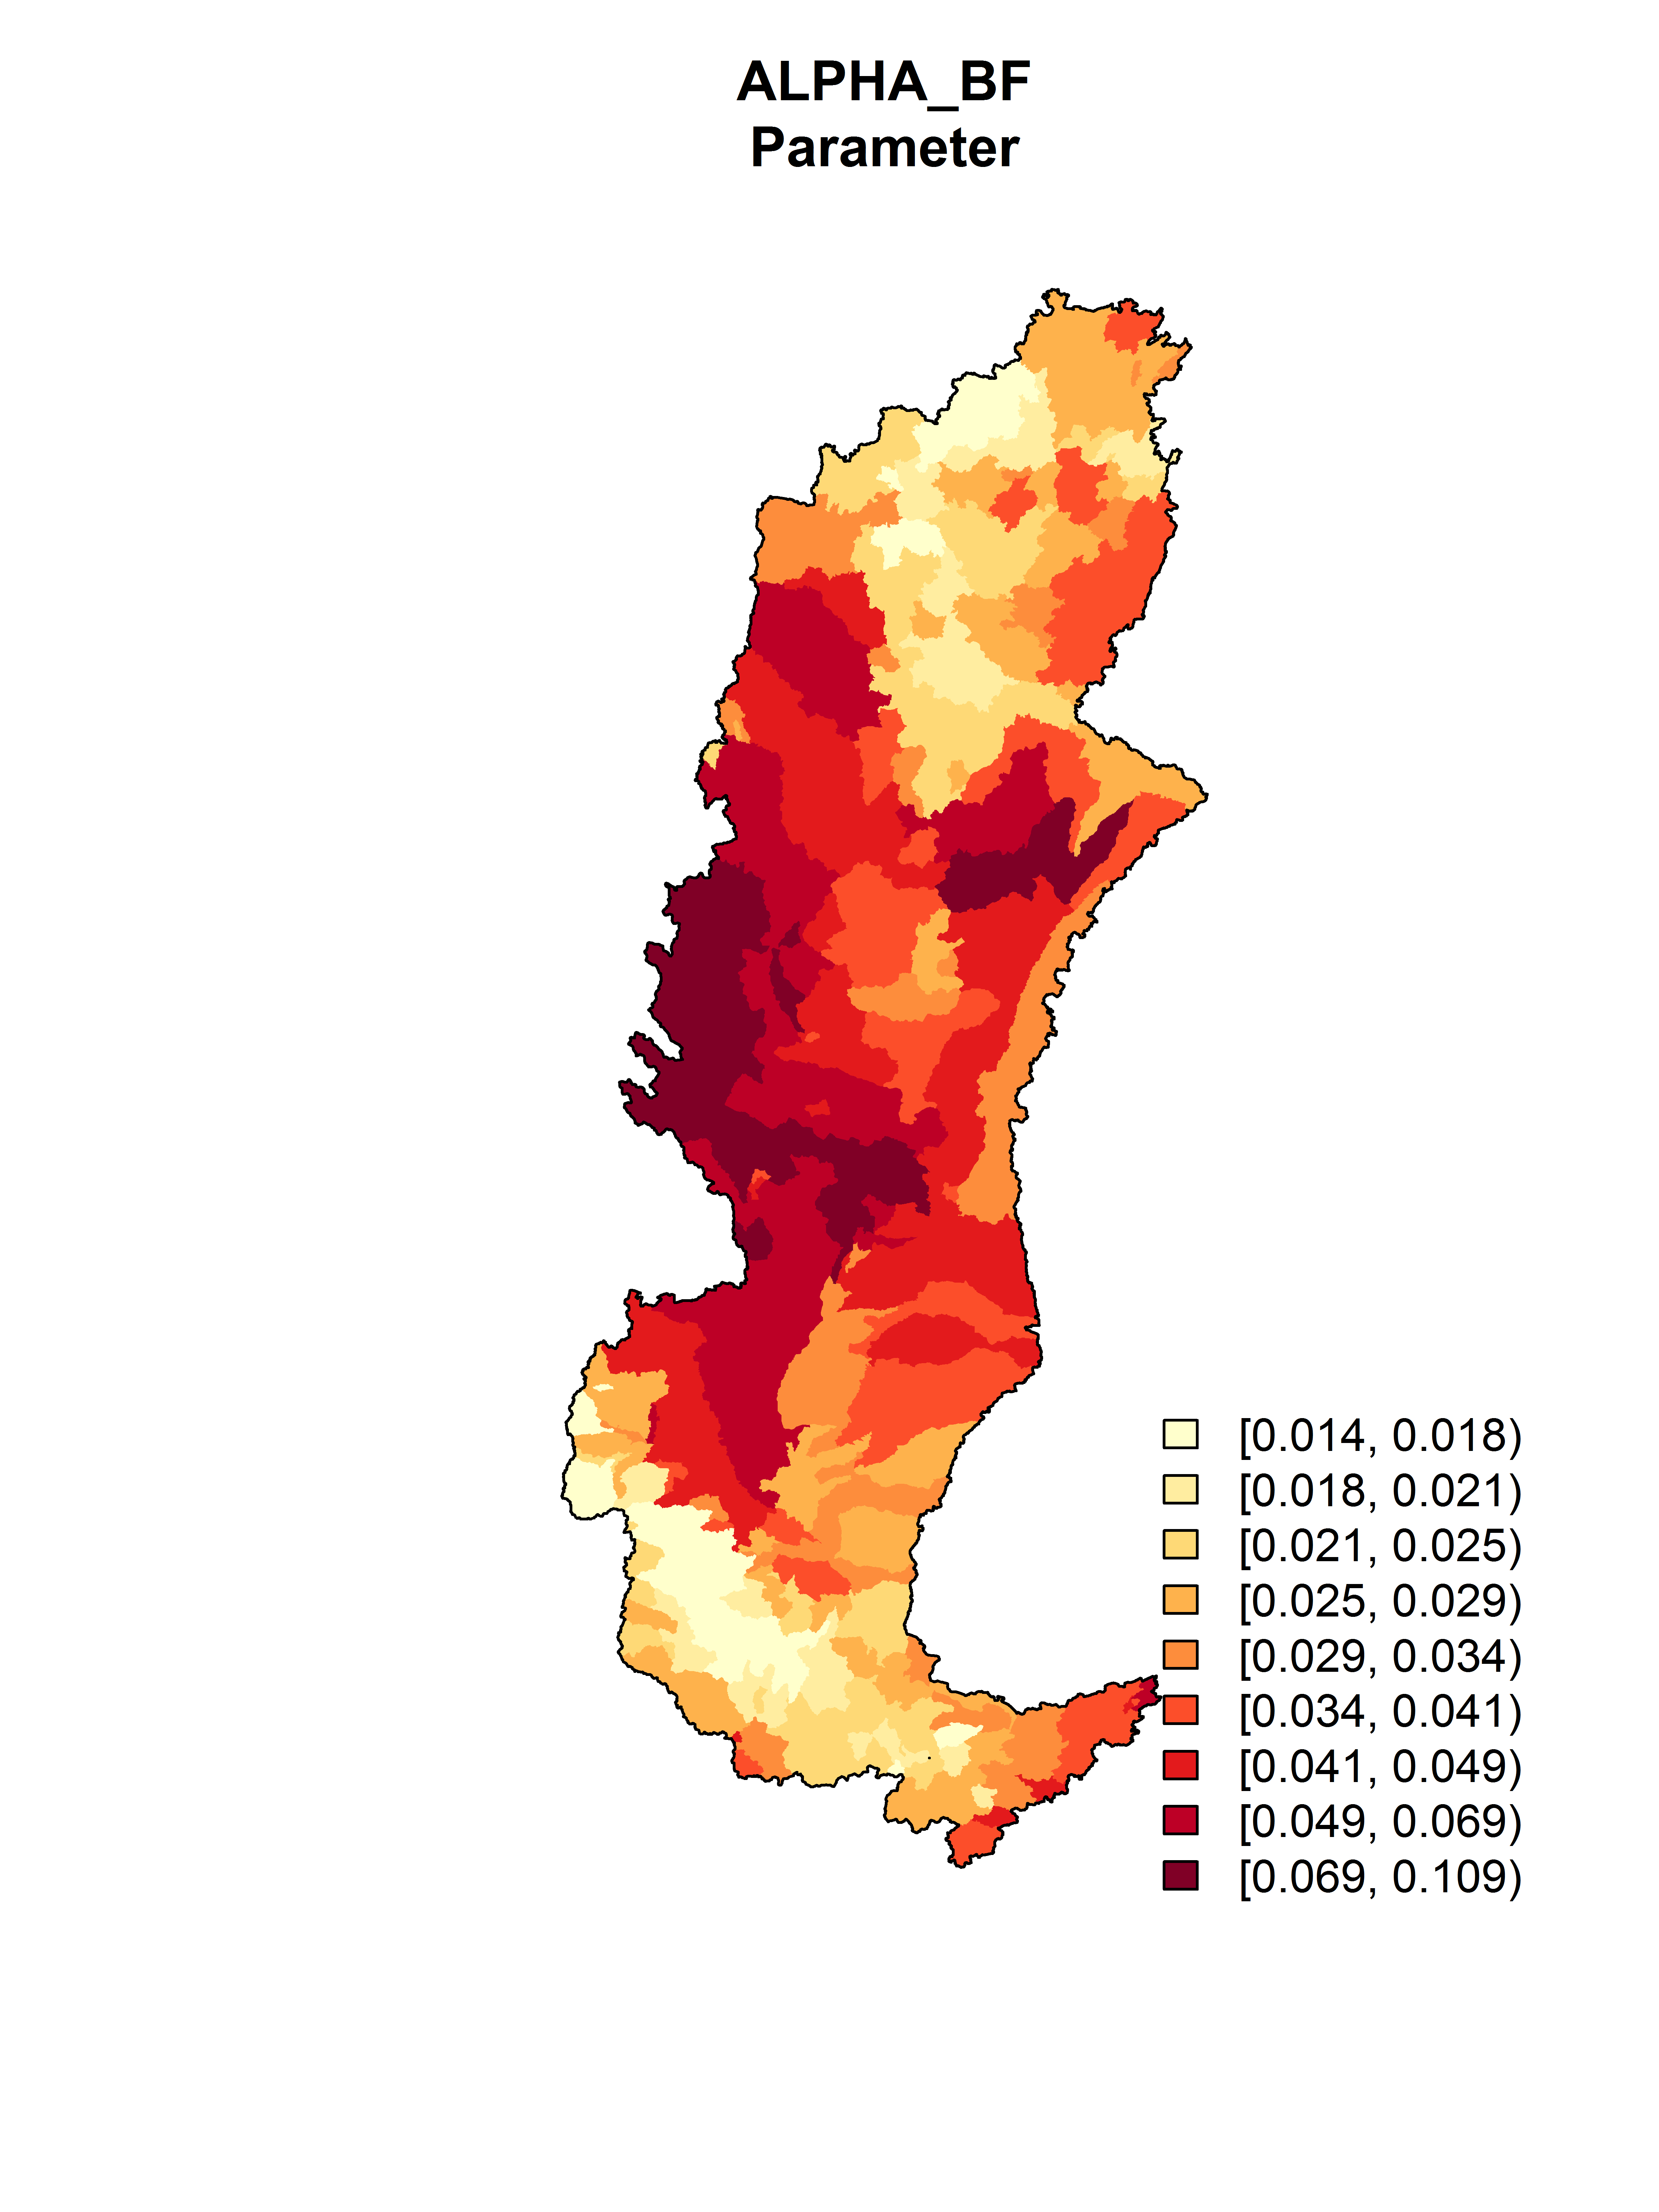
\includegraphics[width=\textwidth]{./img/alpha_bf.png}
	\caption{Map showing the predicted ALPHA\_BF for each SWAT subbasin. Higher (darker) values indicate a high response of groundwater to recharge.}
	\label{fig:alpha_bf}
\end{figure}

%%Groundwater Phophorus
\begin{figure}[h!]
	\centering
	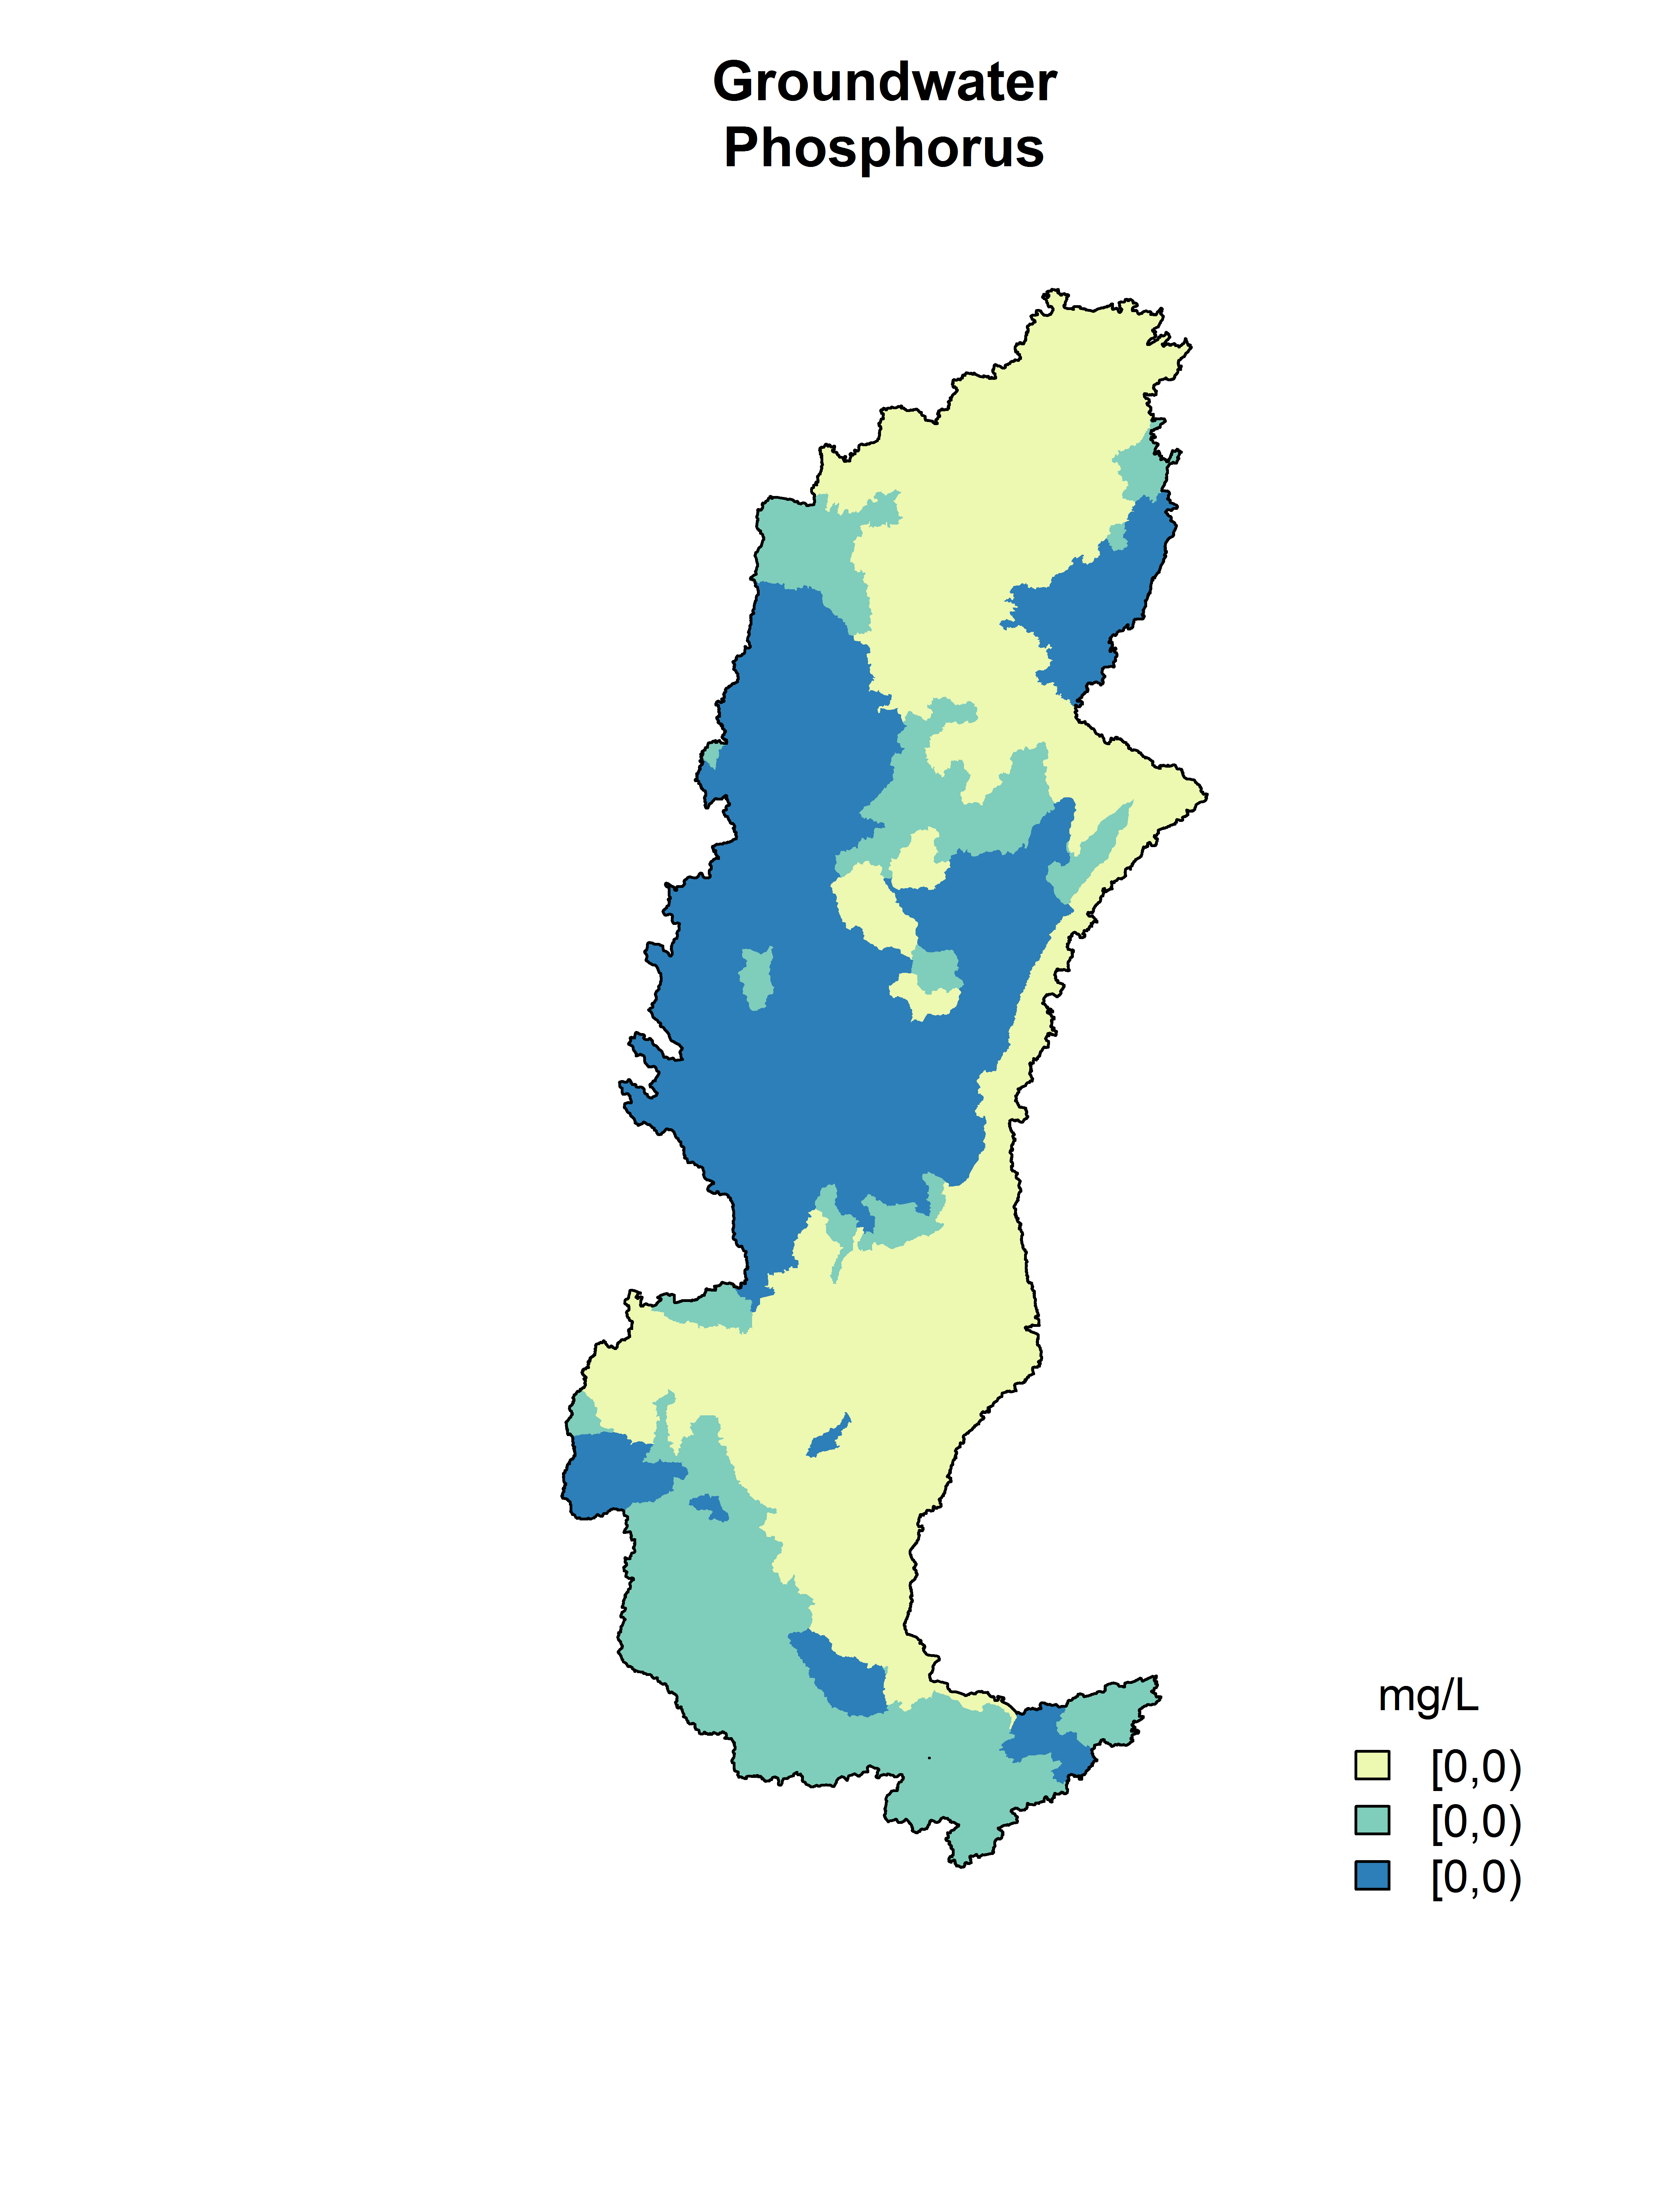
\includegraphics[width=\textwidth]{./img/groundwater_phosphorus.png}
	\caption{Map showing the estimated concentration of groundwater phosphorus in the Wisconsin River Basin. Values were obtained from \citet{robertson_phosphoruszones_2006}}
	\label{fig:groundwater_p}
\end{figure}


%Streamflow calib sites
\begin{figure}[h]
	\centering
	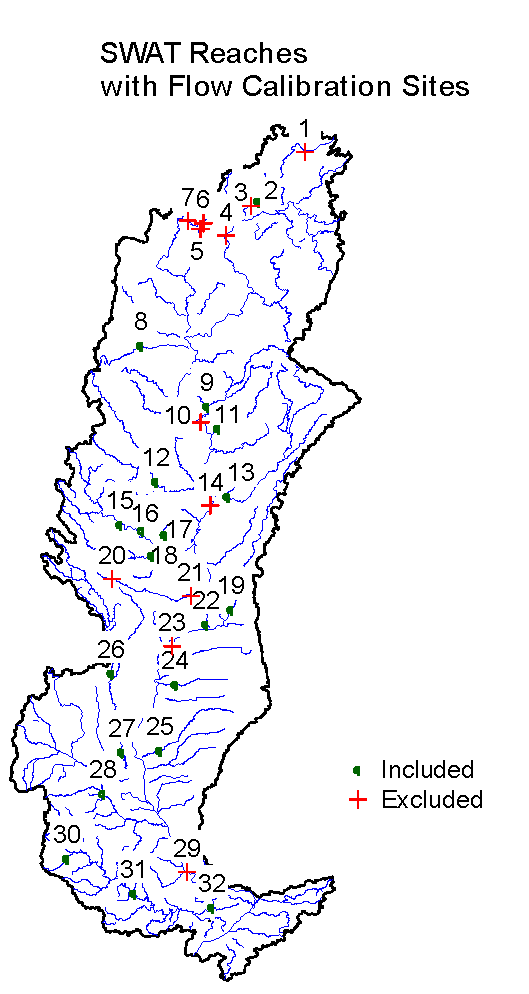
\includegraphics{./img/flow_calib_sites_changed}
	\caption{Flow monitoring sites. The sites marked ``Included'' are currently considered calibration sites. Those marked ``Excluded'' are downstream of reservoirs or other structures that regulate flow and so are not used for calibration. For more detailed information see Table \ref{tab:streamflow_calibration_sites}.}
	\label{fig:calibration_site_map}
\end{figure}
\clearpage